\chapter{Timing Calibration and Validation}

To perform the timing calibration of the AHCAL, the complete muon dataset is used. Table \ref{table:mu_elec_runs} summarizes the runs and datasets used. Raw events are considered if the reference signals T$_{12}$,  T$_{13}$ and T$_{14}$ are present in the event. Raw events are the number of events after the MIP selection. Selected events are counted after the selection on the error of the time reference as explained in \ref{subsection:time_ref}.

\begin{table}[htb!]
	\centering
	\caption{Table with the run statistic before and after selection used for timing calibration.}
	\label{table:mu_elec_runs}
	\resizebox{0.8\textwidth}{!}{%
	\begin{tabular}{@{} llllll @{}}
		\hline
		Runs & Energy & Particle Type & Events (Raw) & Events (sel.) & $\frac{\text{N$_{sel.}$}}{\text{N$_{raw}$}}$ \\
		\hline
		24016-24663 & 50-150 GeV & $\mu^-$ & 1851536 & 836796 & 45.2\% \\
		24528-24577 & 10 GeV & $e^-$ & 268275 & 216656 & 80.8\% \\
		24510-24520 & 15 GeV & $e^-$ & 108092 & 90395 & 83.6\% \\
		24486-24504 & 20 GeV & $e^-$ & 130232 & 110161 & 84.6\% \\
		24460-24470 & 30 GeV & $e^-$ & 82202 & 69692 & 84.8\% \\
		24427-24435 & 40 GeV & $e^-$ & 65901 & 55660 & 84.5\% \\
		24405-24419 & 50 GeV & $e^-$ & 123422 & 104030 & 84.3\% \\
		\hline
	\end{tabular}
	}
\end{table}

The timing calibration is performed in several steps and will be explained in the following sections.
\begin{itemize}
	\item Determination of the timing slope to convert TDC value to nanoseconds.
	\item Calibration of the time reference
	\item Non-linearity correction
	\item Time-walk correction
\end{itemize}

\section{Slope calibration}
\label{subsec:slope_calib}

The data analysis is performed in several steps. The first step is the calibration of the time provided by the \textit{SPIROC2B} chip. To reconstruct the time of the first hit in a channel (only a single hit per channel is registered during a bunch-crossing), the TDC value measured needs to be converted into nanoseconds. The value is converted using the following equations:

\begin{equation} \label{eq:slope}
	\text{slope}_{chip, BXID} \: \text{[ns/TDC]} = \frac{3920 \: \text{ns}}{\text{Max}_{chip, BXID} - \text{Pedestal}_{chip, BXID}}
\end{equation}
\begin{equation} \label{eq:time_chn}
	\text{T}_{chn} \: \text{[ns]} = \text{slope}_{chip, BXID} \times (\text{TDC} - \text{Pedestal}_{mem=1} )
\end{equation}

The slope are calculated separately for odd and even BXID due to the chip design presenting two voltage ramps, one for each BXID parity. The determination of the parameter $\text{slope}_{chip, BXID}$ is assuming that the TDC ramp in the chip is linear to a first order. The parameters Max$_{chip, BXID}$ and Pedestal$_{chip, BXID}$ in eq.\ref{eq:slope} are extracted from the TDC spectrum for a specific chip and BXID using only the first memory cell as illustrated in figure \ref{fig:TDC_Spectrum}. At the same time, the parameter Pedestal$_{mem=1}$ in eq.\ref{eq:time_chn} is extracted from the spectrum for each channel and the first memory cell of a chip without taking into account the BXID of the ramp. The difference between both pedestals and for the other memory-cells will be corrected for at a later stage. This is accounting for a total of 208 slopes and 3744 pedestals to be extracted for the testbeam setup.

\begin{figure}[htbp!]
	\begin{subfigure}[t]{0.5\textwidth}
		\centering
		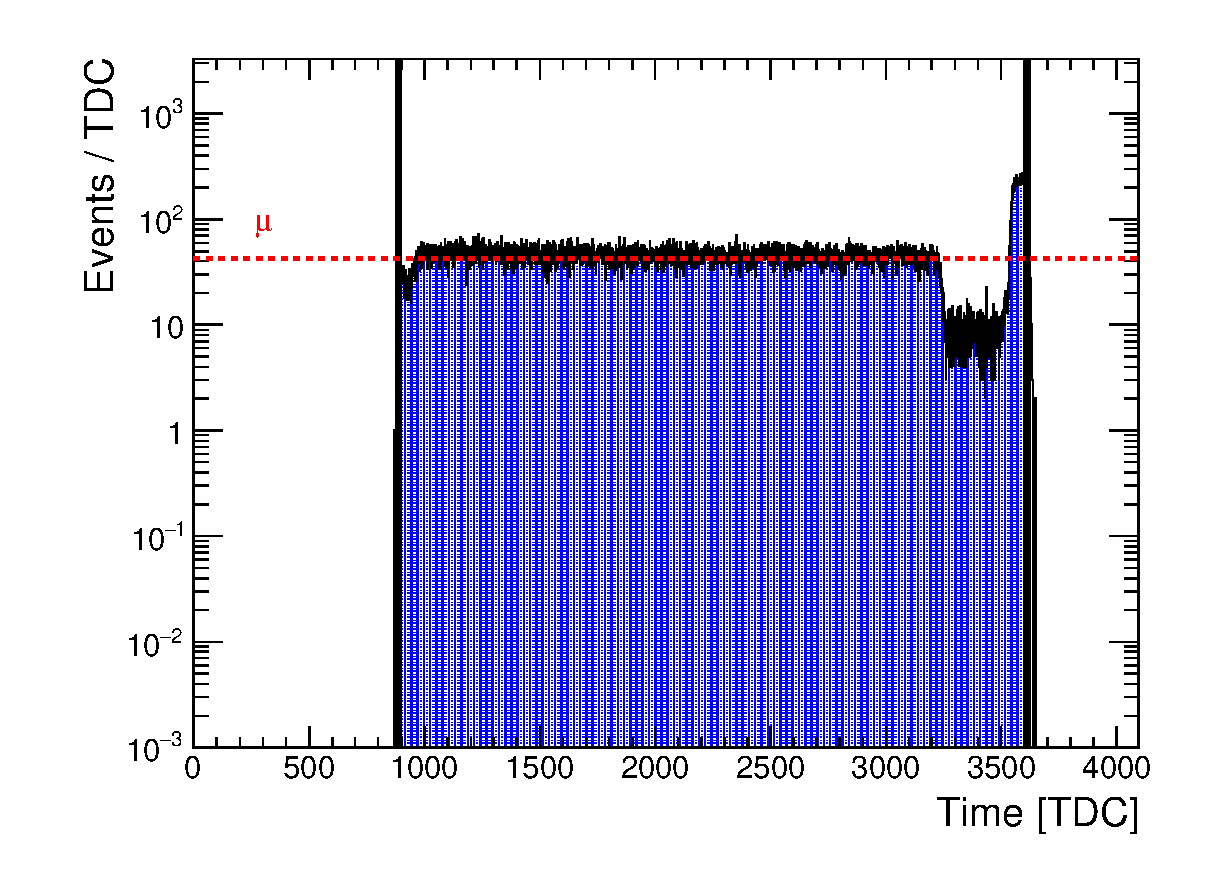
\includegraphics[width=1\linewidth]{../Thesis_Plots/Timing/Muons/Plots/ExampleTDCSpectra}
		\caption{TDC Spectrum of a typical chip.} \label{fig:TDC_Spectrum}
	\end{subfigure}
	\hfill
	\begin{subfigure}[t]{0.5\textwidth}
		\centering
		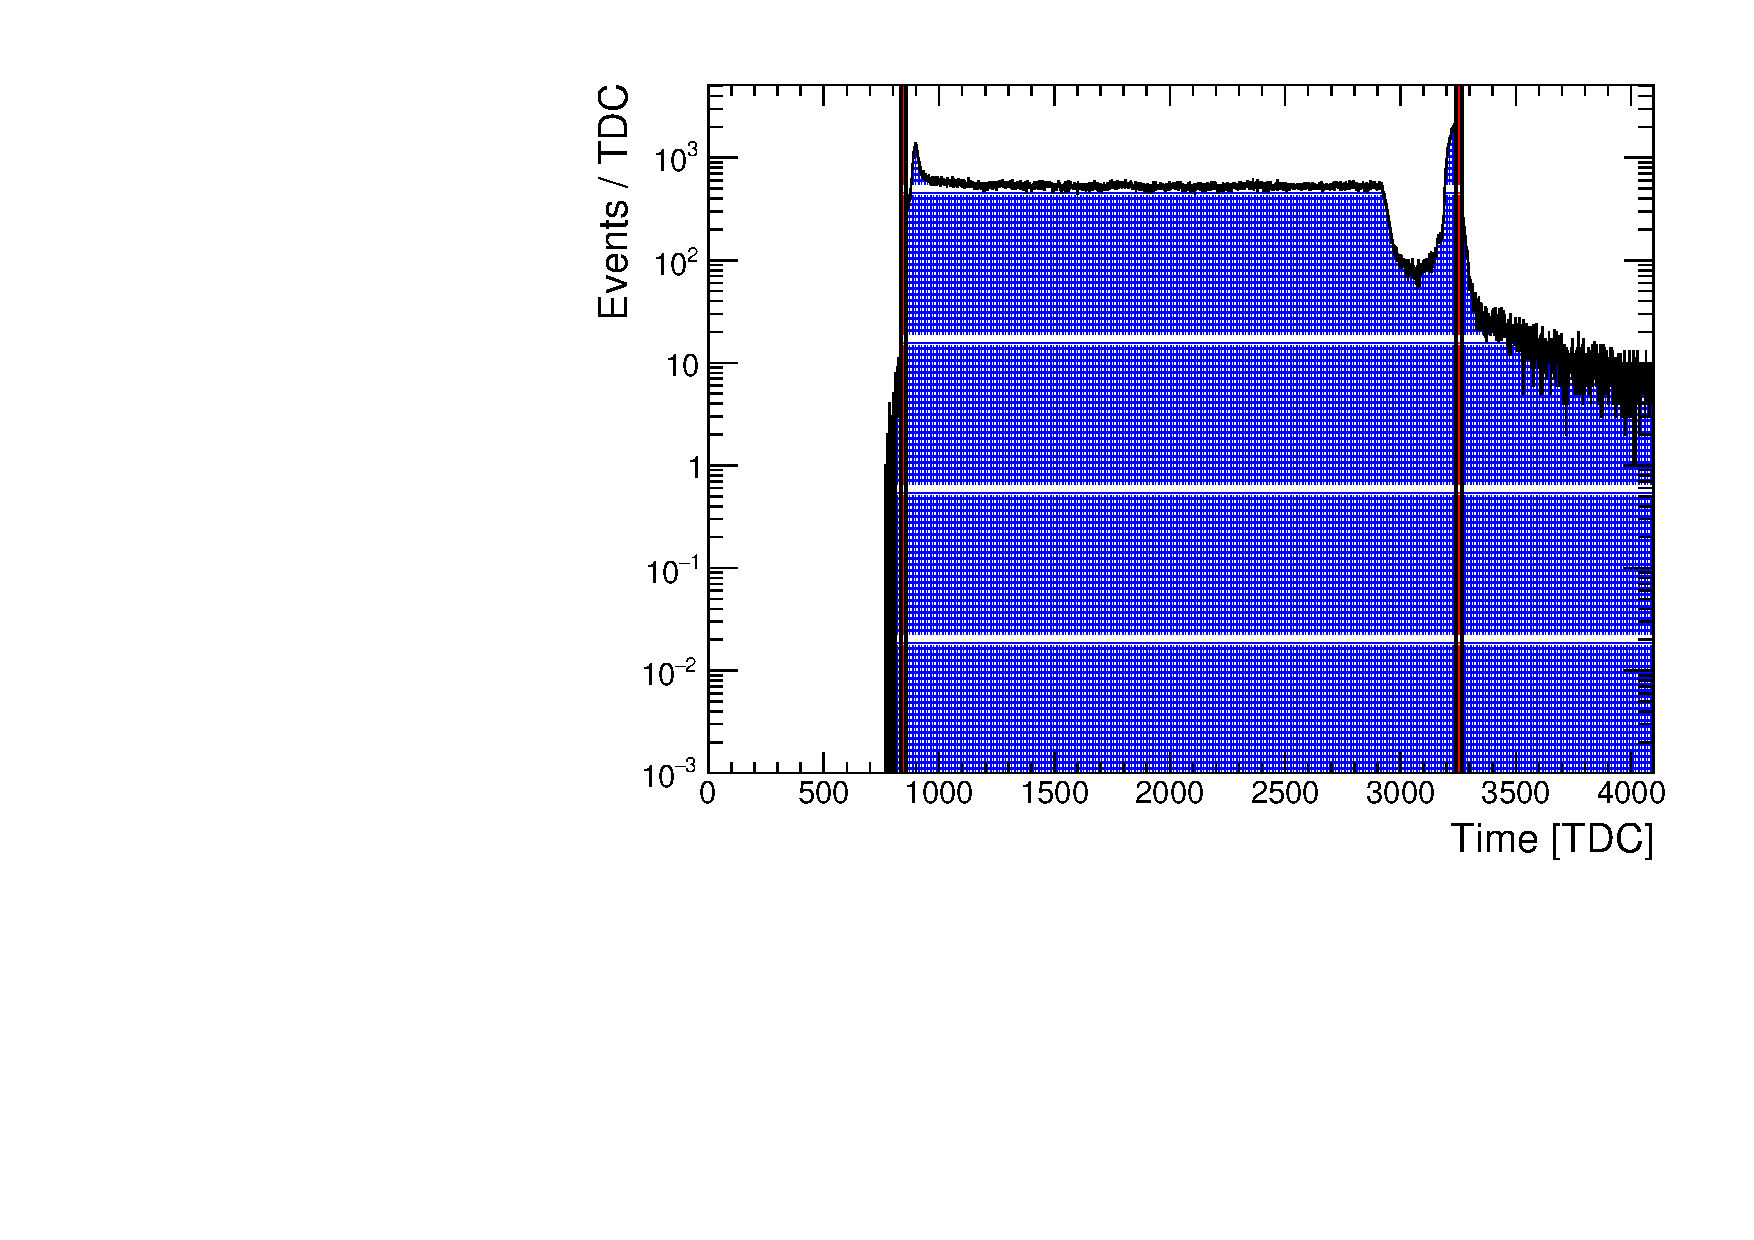
\includegraphics[width=1\linewidth]{../Thesis_Plots/Timing/Muons/Plots/BadTDCSpectra_Layer12}
		\caption{TDC Spectrum of a bad chip on layer 12.} \label{fig:TDC_Spectrum_bad}
	\end{subfigure}
	\caption{\subref{fig:TDC_Spectrum}) The black lines indicate the fitted Max and Pedestal parameters for this chip. The yellow bands represents estimation of the uncertainty on the extraction of the parameters by a variation of 1 RMS of the threshold $\mu$. slope = 1.56 $\pm$ 0.01, Pedestal = 816 $\pm$ 9 and Maximum = 3336 $\pm$ 8. \subref{fig:TDC_Spectrum_bad}) An example of a bad chip (Chip 190) on layer 12 presenting a long tail to high TDC values. The reason is not totally understood but present on all chips on that layer.}
\end{figure}
The technique of extraction is based on an edge detection method. For each chip and BXID, an histogram is filled with the y value of each bin. Then the mean of this histogram is defined as a threshold $\mu$. The parameter Pedestal$_{chip, BXID}$ is extracted as the first bin above 30\% of $\mu$. For the parameter Max$_{chip, BXID}$, it is extracted as the last bin above 50\% of the highest bin $BinMax$ of the original histogram. The maximum seems not to be exactly at the last bin of the spectrum, this is due to the technique that needed to be robust against strange spectra as shown in figure \ref{fig:TDC_Spectrum_bad}.
An estimation of the uncertainties on the pedestal $\sigma_{Ped}$ and maximum $\sigma_{Max}$ is done by the following formulas:
\begin{equation} \label{eq:errorPed}
	\begin{aligned}
		\sigma_{Ped} \: = & \: \text{max}(\left|\text{FirstBinAbove}(\mu - RMS) \times 0.3 - \text{Pedestal}_{chip, BXID}\right|, \\
		& \left|\text{FirstBinAbove}(\mu + RMS) \times 0.3 - \text{Pedestal}_{chip, BXID}\right|)
	\end{aligned}
\end{equation}
\begin{equation} \label{eq:errorMax}
	\begin{aligned}
		\sigma_{Max} \: = & \: \text{max}(\left|\text{LastBinAbove}(BinMax - 0.33 \times BinMax) \times 0.5 - \text{Max}_{chip, BXID}\right|, \\
		& \left|\text{LastBinAbove}(BinMax - 0.33 \times BinMax) \times 0.5 - \text{Max}_{chip, BXID}\right|)
	\end{aligned}
\end{equation}
More details about the estimation of the calibration uncertainties is described in the appendix \ref{appendix:calib_error}. The extracted values for the slopes are shown in figure \ref{fig:slope_time}. They are in the expected range of 1.6 ns per TDC bin due to the limited dynamic range provided by the chip (around 2500 bins for 4 $\mu$s).

\begin{figure}[htbp!]
	\centering
	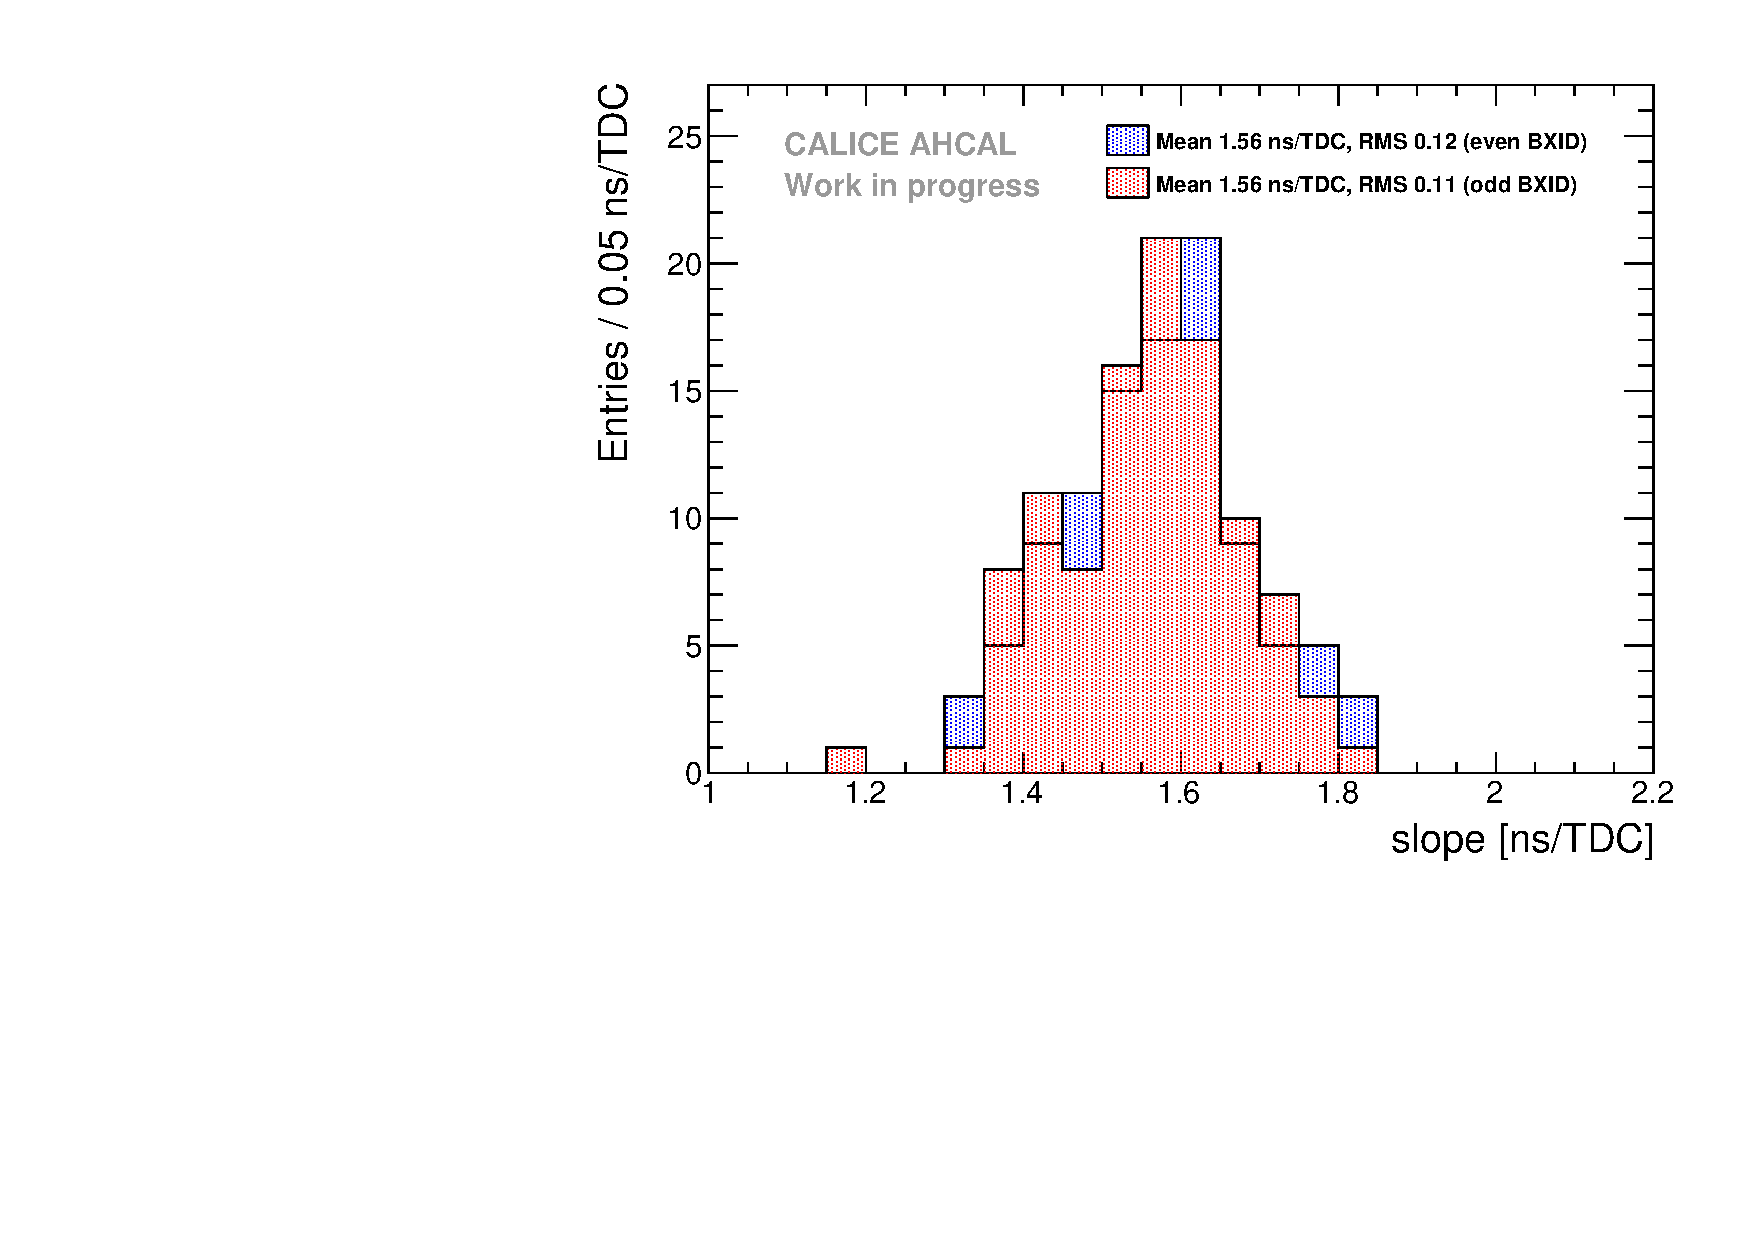
\includegraphics[width=0.7\linewidth]{../Thesis_Plots/Timing/Muons/Plots/SlopesTDC}
	\caption{Distribution of the fitted slopes for even and odd bunch-crossing IDs. $\mu_{odd}$ = 1.564 ns/TDC, RMS$_{odd}$ = 0.121, $\mu_{even}$ = 1.556 ns/TDC, RMS$_{even}$ = 0.113. In total, 208 TDC slopes were extracted.} \label{fig:slope_time}
\end{figure}

\section{Calibration of the time reference}
\label{section:time_ref}

To reconstruct the time of the first hit in a channel, the measured time of a hit needs to be compared to the time of a reference trigger. The trigger signals described in subsection \ref{subsec:trigger} are calibrated using the same method as explained above with the addition that the values for all memory cells are extracted separately, possible due to the high statistics in these channels, for these channels to guaranty the most accurate result.

\begin{figure}[htbp!]
	\begin{subfigure}[t]{0.5\textwidth}
		\centering
		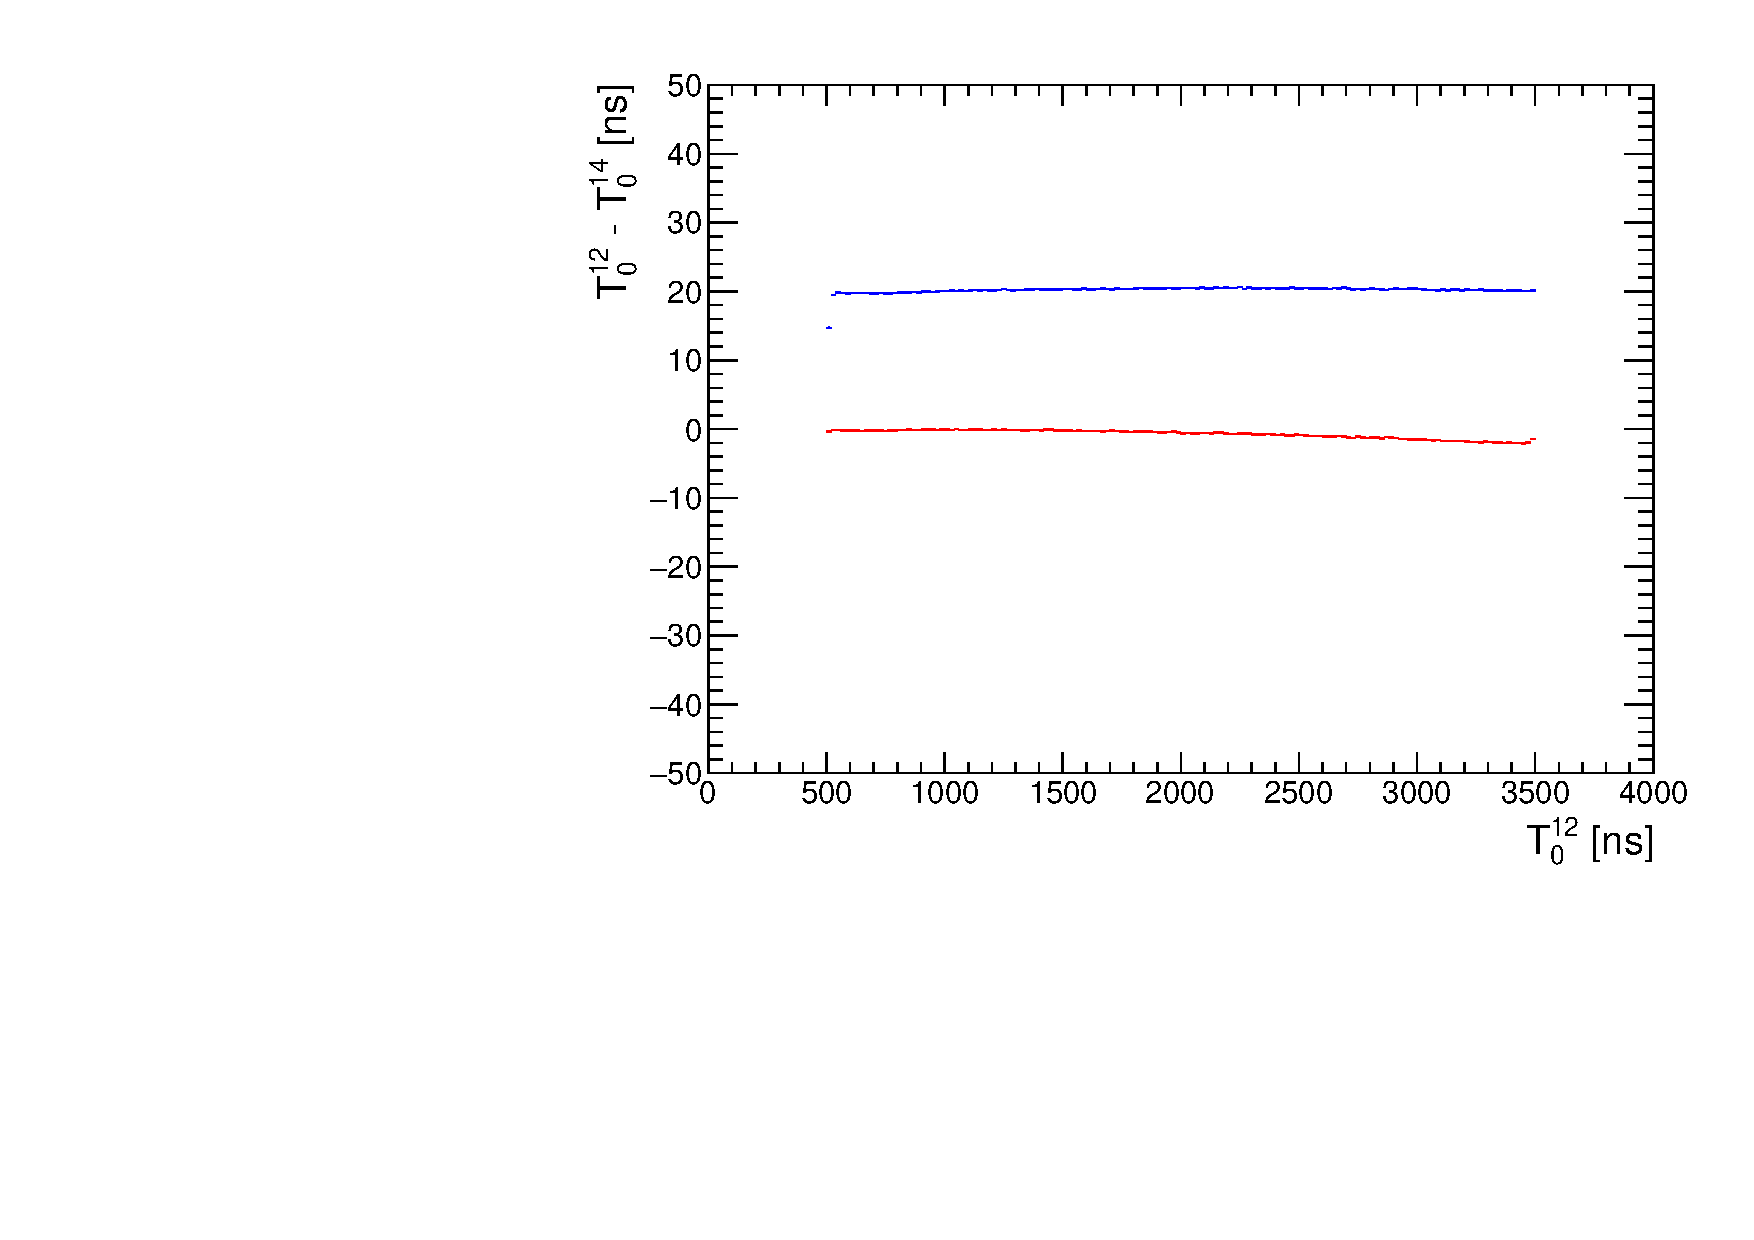
\includegraphics[width=1\linewidth]{../Thesis_Plots/Timing/T0s/Plots/Profiles_DeviationT0_12_14}
		\caption{Profile of the difference between T$_{12}$ and T$_{14}$ before correction.} \label{fig:DeviationProfileT0s}
	\end{subfigure}
	\hfill
	\begin{subfigure}[t]{0.5\textwidth}
		\centering
		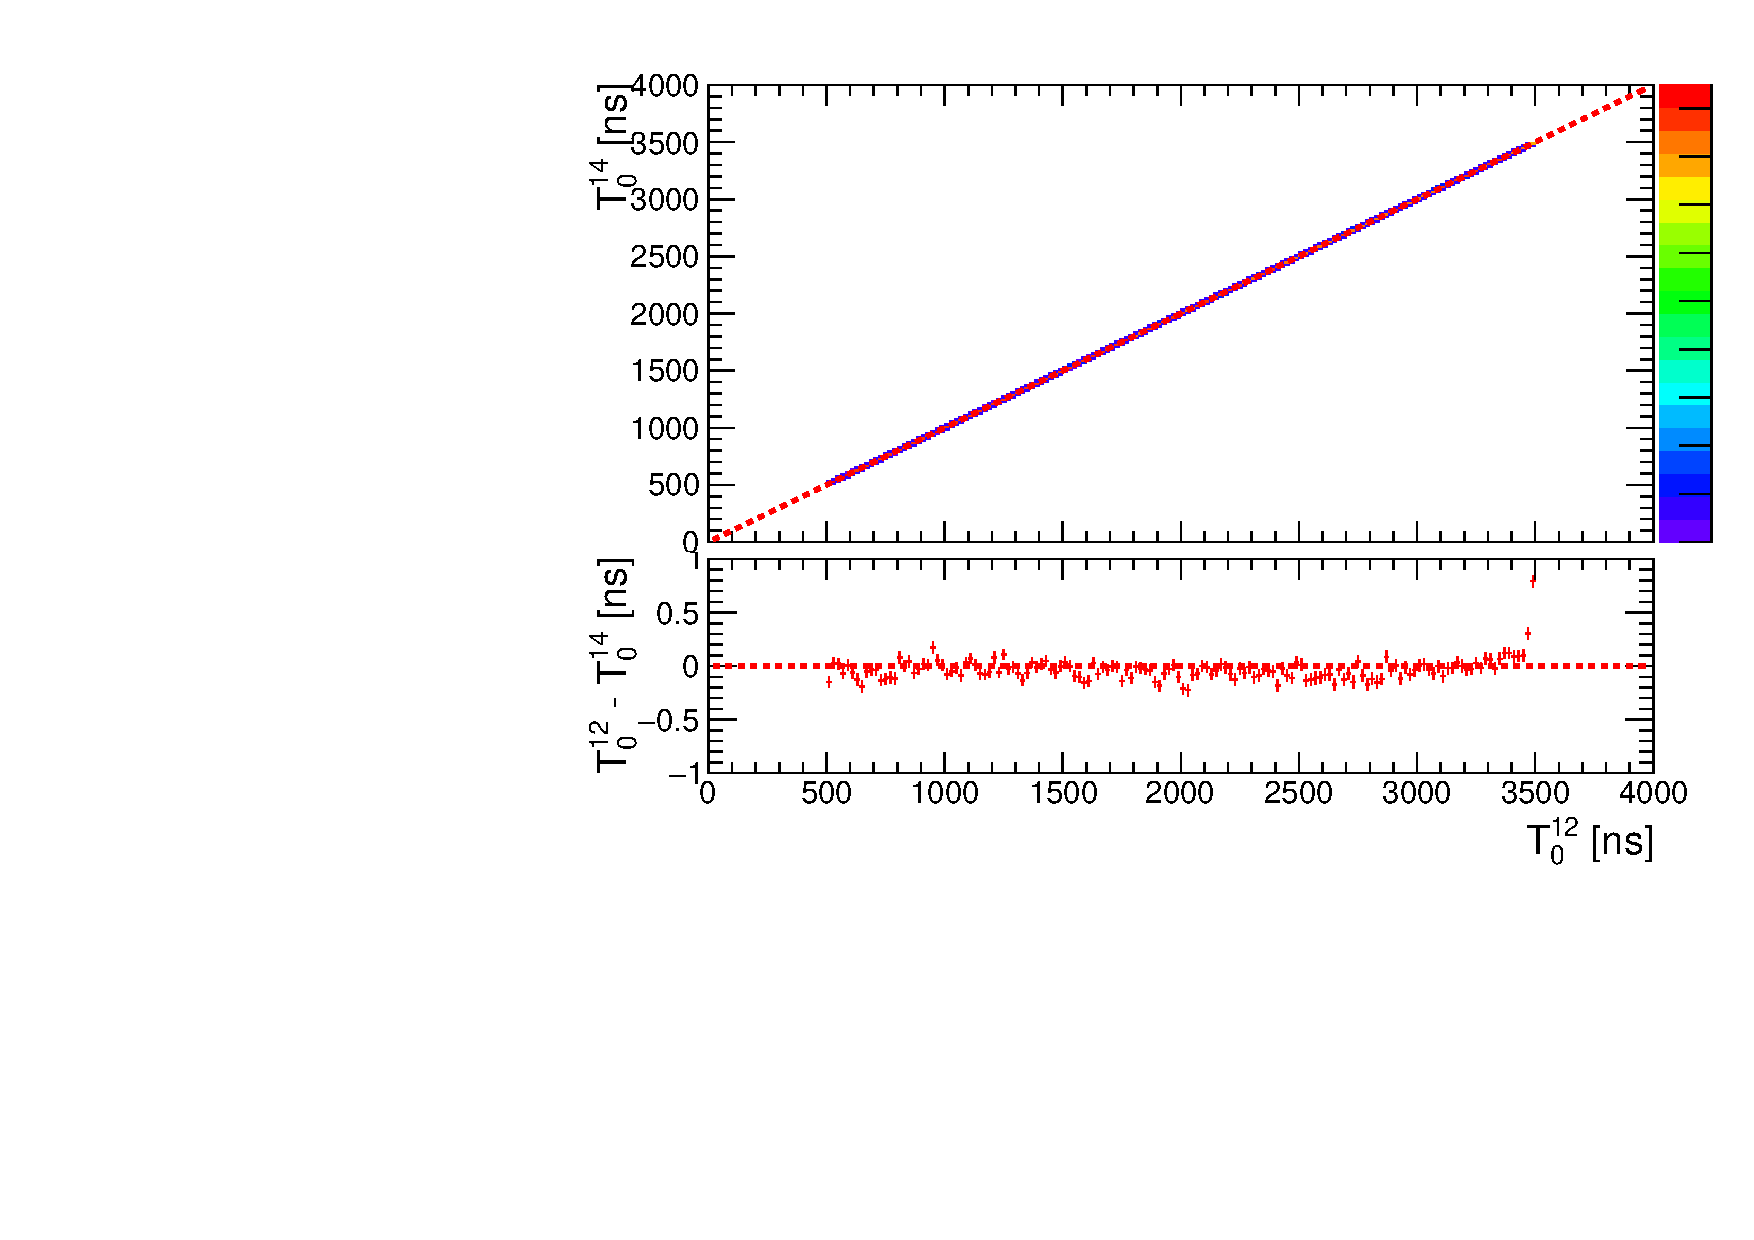
\includegraphics[width=1\textwidth]{../Thesis_Plots/Timing/T0s/Plots/Correlation_T12vsT14_TDC2ns.pdf}
		\caption{Time correlation the reference triggers T$_{12}$ and T$_{14}$.}\label{fig:Corr_T12T14}
	\end{subfigure}
	\caption{\subref{fig:DeviationProfileT0s} .\subref{fig:Corr_T12T14}) The top left plot shows the time correlation between the references T$_{12}$ and T$_{14}$ after correction. An additionnal cut on the time between 500 and 3500 ns is done. The bottom plot show the profile of the difference between them.}
\end{figure}

After time calibration of the calorimeter hits, events are selected by requiring that T$_{12}$, T$_{13}$ and T$_{14}$ are present in the event in a certain amplitude range (see appendix \ref{}) to reject noise hits from these channels. In addition, as these channels receive exactly the same signal from the NIM-logic at the same time, a correction is applied to ensure that they match in time. The correction is performed by correcting the time of T$_{12}$ and T$_{13}$ compared to the time of T$_{14}$ as shown in figure \ref{fig:DeviationProfileT0s}.
After correction, the figure \ref{fig:Corr_T12T14} shows the correlation between T$_{12}$ and T$_{14}$. The figure \ref{fig:T0_Correction} shows that the correction reduces the difference of the trigger channels w.r.t to each other. This is certainly due to the fact that a different value of the pedestal is needed for each BXID parity which was not expected. The resulting width for the reference trigger signal is around 4-5 ns. This resolution from the electronics contributes to the final timing resolution obtained.

\begin{figure}[htbp!]
	\begin{subfigure}[t]{0.5\textwidth}
		\centering
		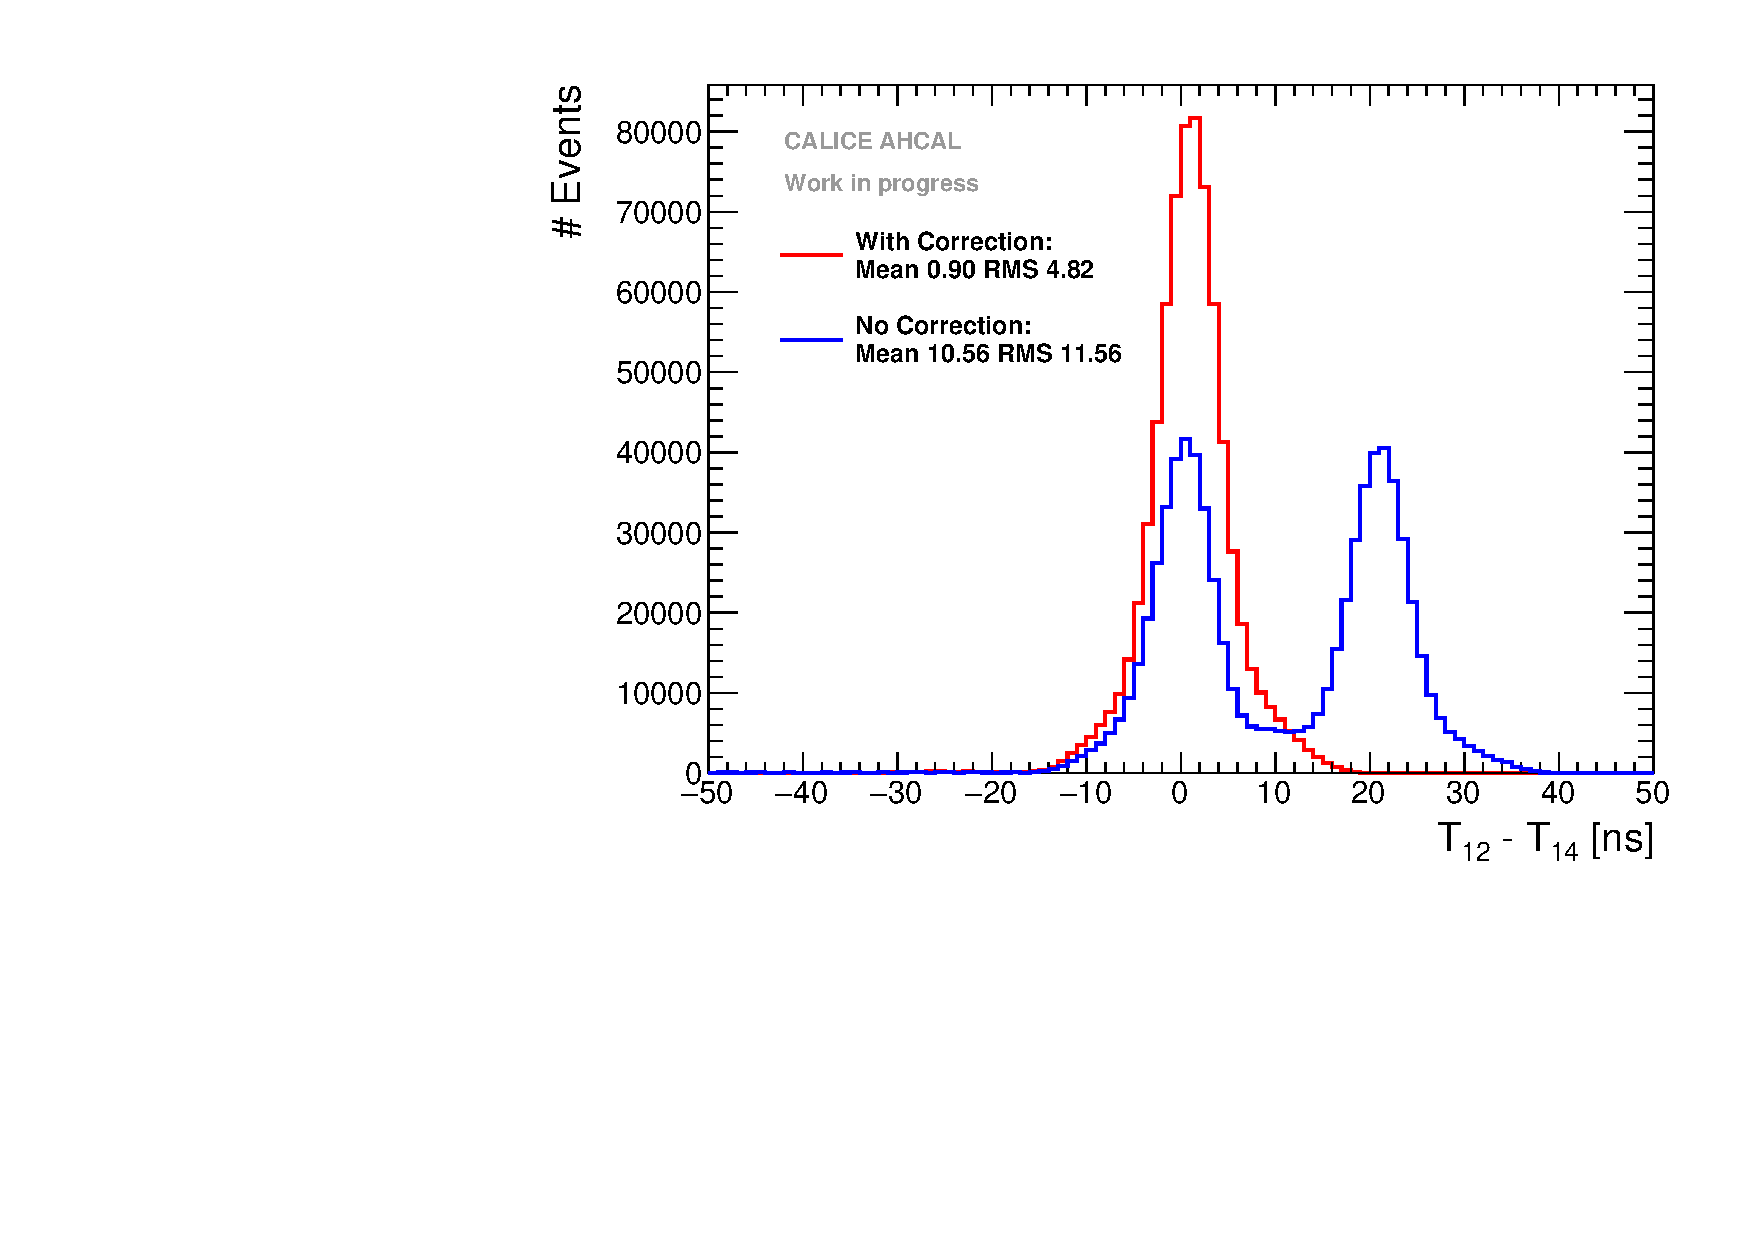
\includegraphics[width=1\textwidth]{../Thesis_Plots/Timing/T0s/Plots/T0_Resolution_5.pdf}
		\caption{Time difference between the trigger channels before and after correction for T$_{12}$ and T$_{14}$.}	\label{fig:T0_Correction}
	\end{subfigure}
	\hfill
	\begin{subfigure}[t]{0.5\textwidth}
		\centering
		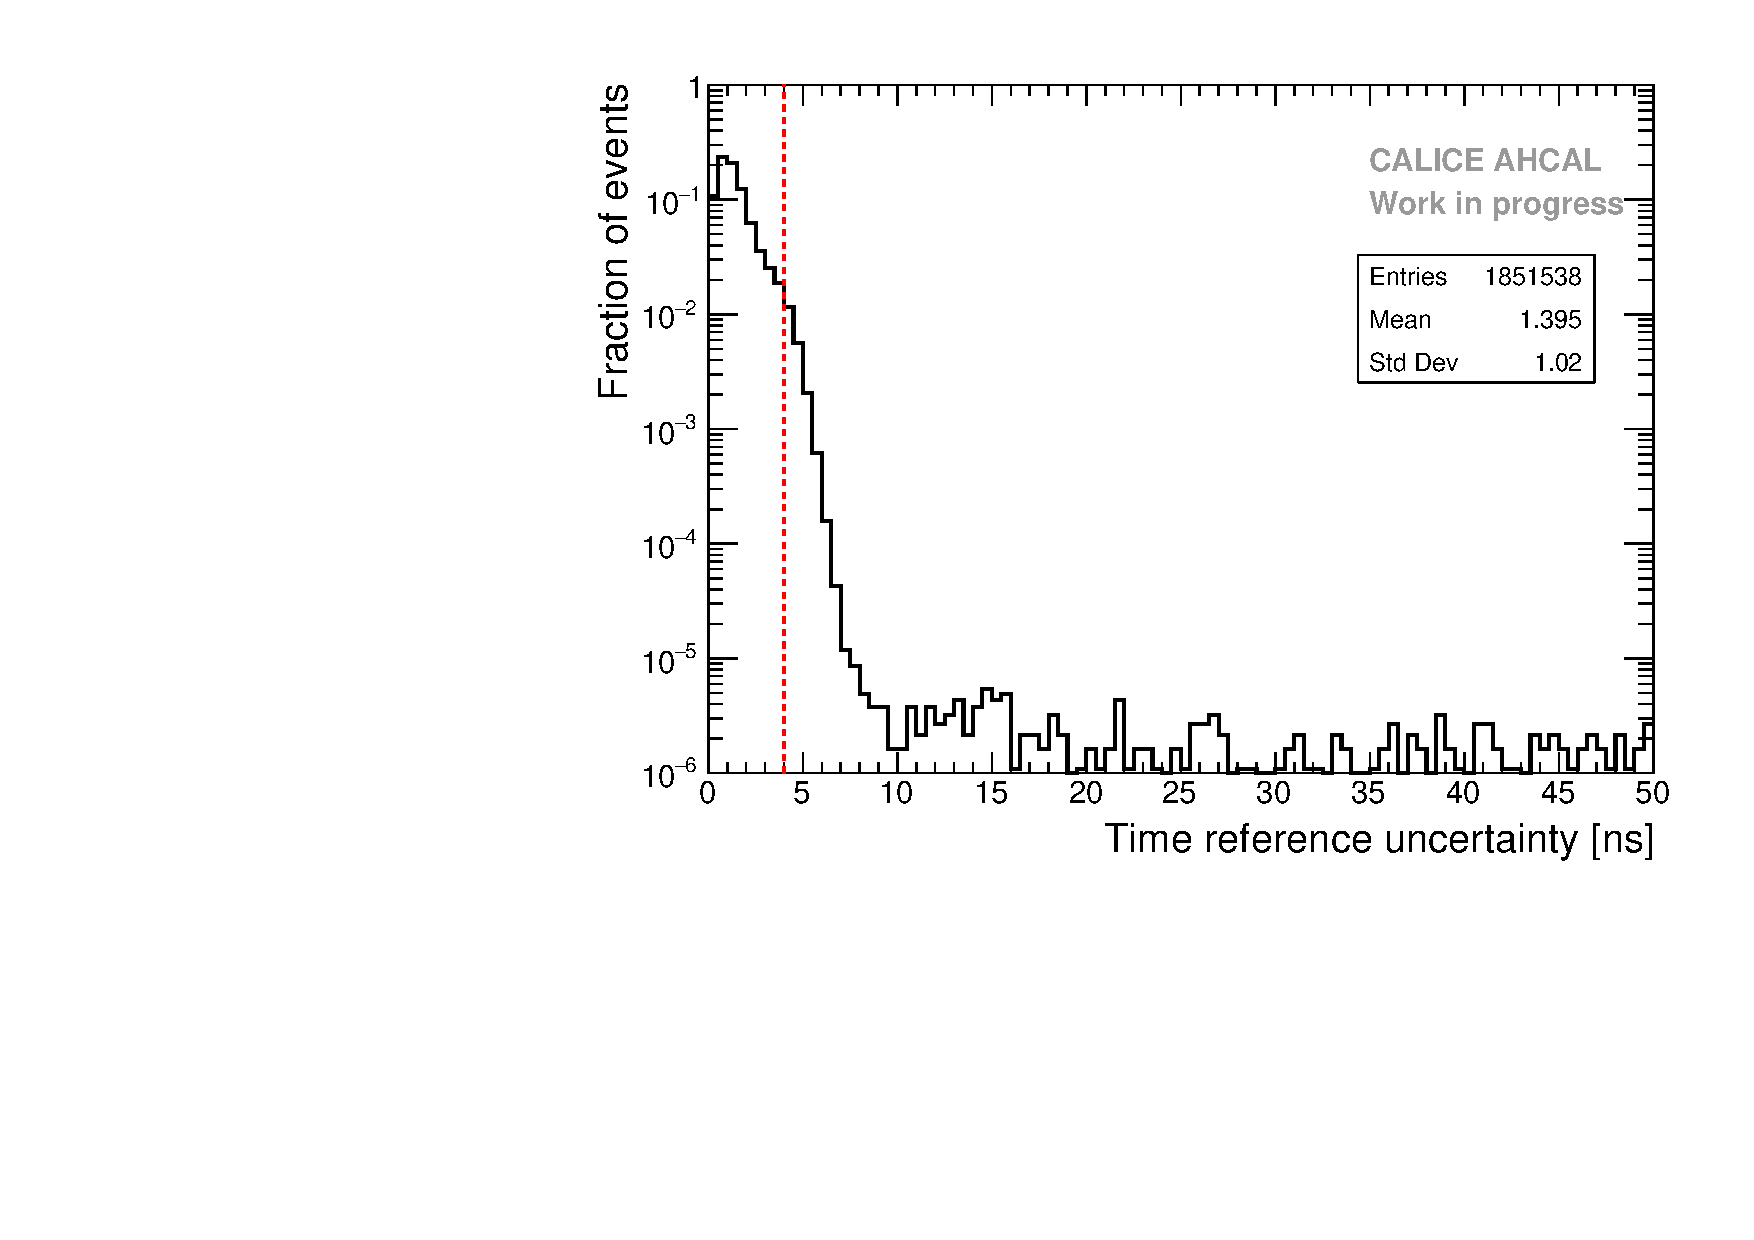
\includegraphics[width=1\linewidth]{../Thesis_Plots/Timing/T0s/Plots/T0ReferenceError}
		\caption{Distribution of the uncertainty $\sigma_{ref}$. The red line represents the cut of 4 ns.} \label{fig:T0ReferenceError}
	\end{subfigure}
	\caption{\subref{fig:T0_Correction}) The histogram in blue shows the difference between the channels before correction, the histogram in red shows the difference after correction. $\mu$ = 10.6 ns, RMS = 11.6 ns, $\mu_{corrected}$ = 0.9 ns, RMS$_{corrected}$ = 4.8 ns. The two visible peaks in blue are due to pedestal values being different dependent of the bunch-crossing parity. \subref{fig:T0ReferenceError}}
\end{figure}

In a next step, to reduce the uncertainty made on the time of the trigger, the time reference $T_{ref}$ is calculated using the mean of T$_{12}$, T$_{13}$ and T$_{14}$ and its associated uncertainty $\sigma_{ref}$ as shown in eq. \ref{eq:tref} \& \ref{eq:tref_err}. A cut of 4 ns is performed on $\sigma_{ref}$ to reject events with a too large uncertainty on the time of the trigger reference as shown in figure \ref{fig:T0ReferenceError}. Finally only hits with a calibrated time value between 500 and 3500 were considered to avoid ramp edge effects.

\begin{equation} \label{eq:tref}
	\text{T}_{ref} = \frac{\text{T}_{12} + \text{T}_{13} + \text{T}_{14}}{3}
\end{equation}
\begin{equation} \label{eq:tref_err}
	\sigma_{ref}^2 = \frac{ (\text{T}_{12} - \text{T}_{ref})^2 + (\text{T}_{13} - \text{T}_{ref})^2  + (\text{T}_{14} - \text{T}_{ref})^2 }{6}
\end{equation}

\section{Determination of the time of first hit}

Since the absolute time between the passage of a muon and the trigger of a channel is not known a priori due to cabling and the trigger electronics, the time offset relative to the trigger is determined from data. Muons are quasi-instantaneous particles thus the time of the first hit distribution for each channel, memory cells and BXID should peak at \textit{t=0}. This shifting procedure takes into account the delay time of the trigger due to cabling and the NIM-logic as well as possible mis-calibrations in pedestals. Only memory-cells containing more than 100 events are considered. This is achieved getting the maximum bin for each channel and memory-cell and iteratively changing the range of the histogram until the RMS of the distribution is under 10 ns. This value was arbitrary chosen. Once a RMS under 10 is reached, the mean of the histogram is taken as the offset value. In a second step, non-prompt events are tagged by requiring at least 4 prompt hits in the range of -20 to 20 ns to account for possible mis-calibration in the first step of determining the offset. This was necessary to remove noisy channels and ensure a good calibration of the offset. The procedure is iterated then once again with the non-prompt events removed and the offset is extracted using the same method as described above.

In this way, 18338 individual offsets are extracted from data. A distribution of the extracted offsets using muon data can be seen in figure \ref{fig:offset_trigger_distribution}. The mean value of -150 ns is in the expected order for the cabling and NIM-logic delay. The figure \ref{fig:BXID_offset} shows that individual offsets have to be extracted for each BXID parity and indicates that a pedestal value per BXID parity is needed to be taken into account in the calibration.

\begin{figure}[htbp!]
	\begin{subfigure}[t]{0.5\textwidth}
		\centering
		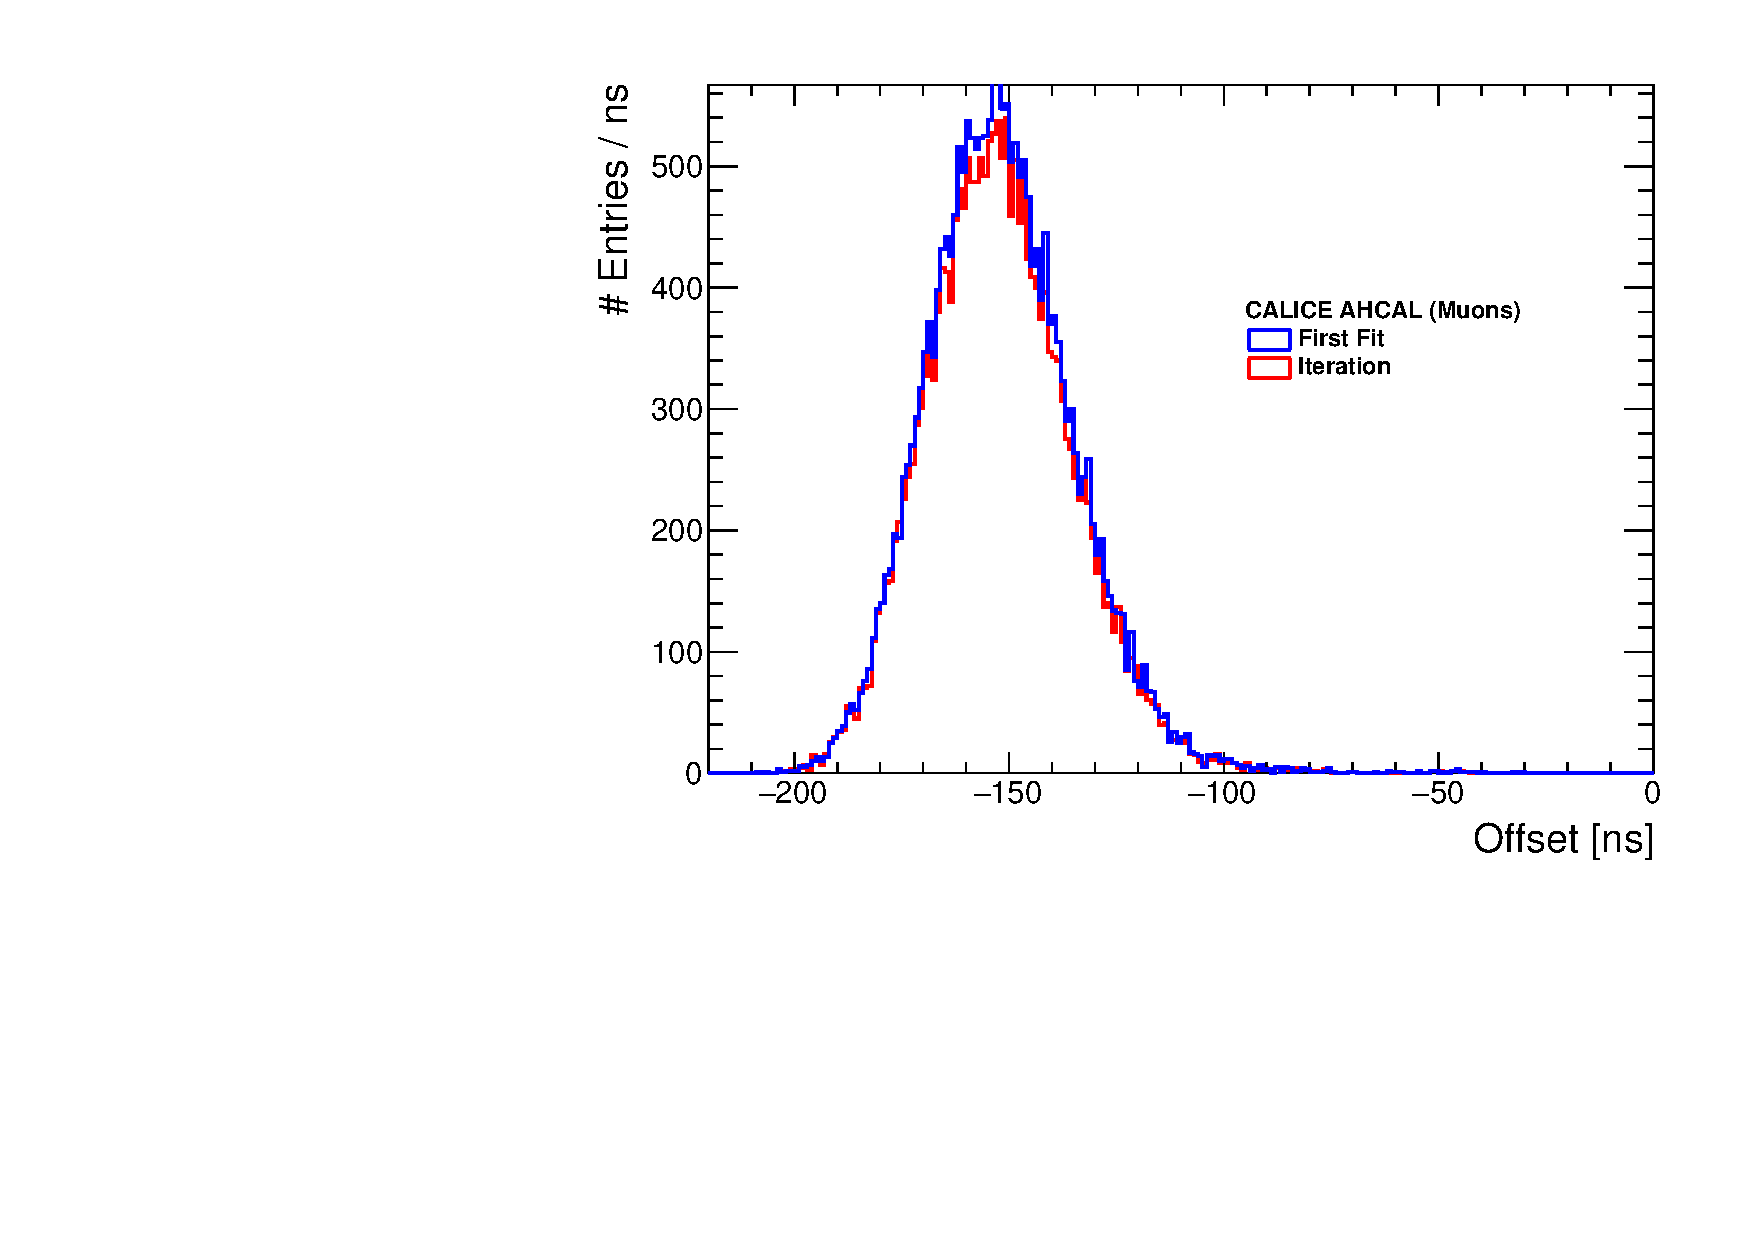
\includegraphics[width=1\textwidth]{../Thesis_Plots/Timing/Muons/Plots/ExtractedOffsets.pdf}
		\caption{Distribution of the offset used to correct for the trigger delay.}\label{fig:offset_trigger_distribution}
	\end{subfigure}
	\hfill
	\begin{subfigure}[t]{0.5\textwidth}
		\centering
		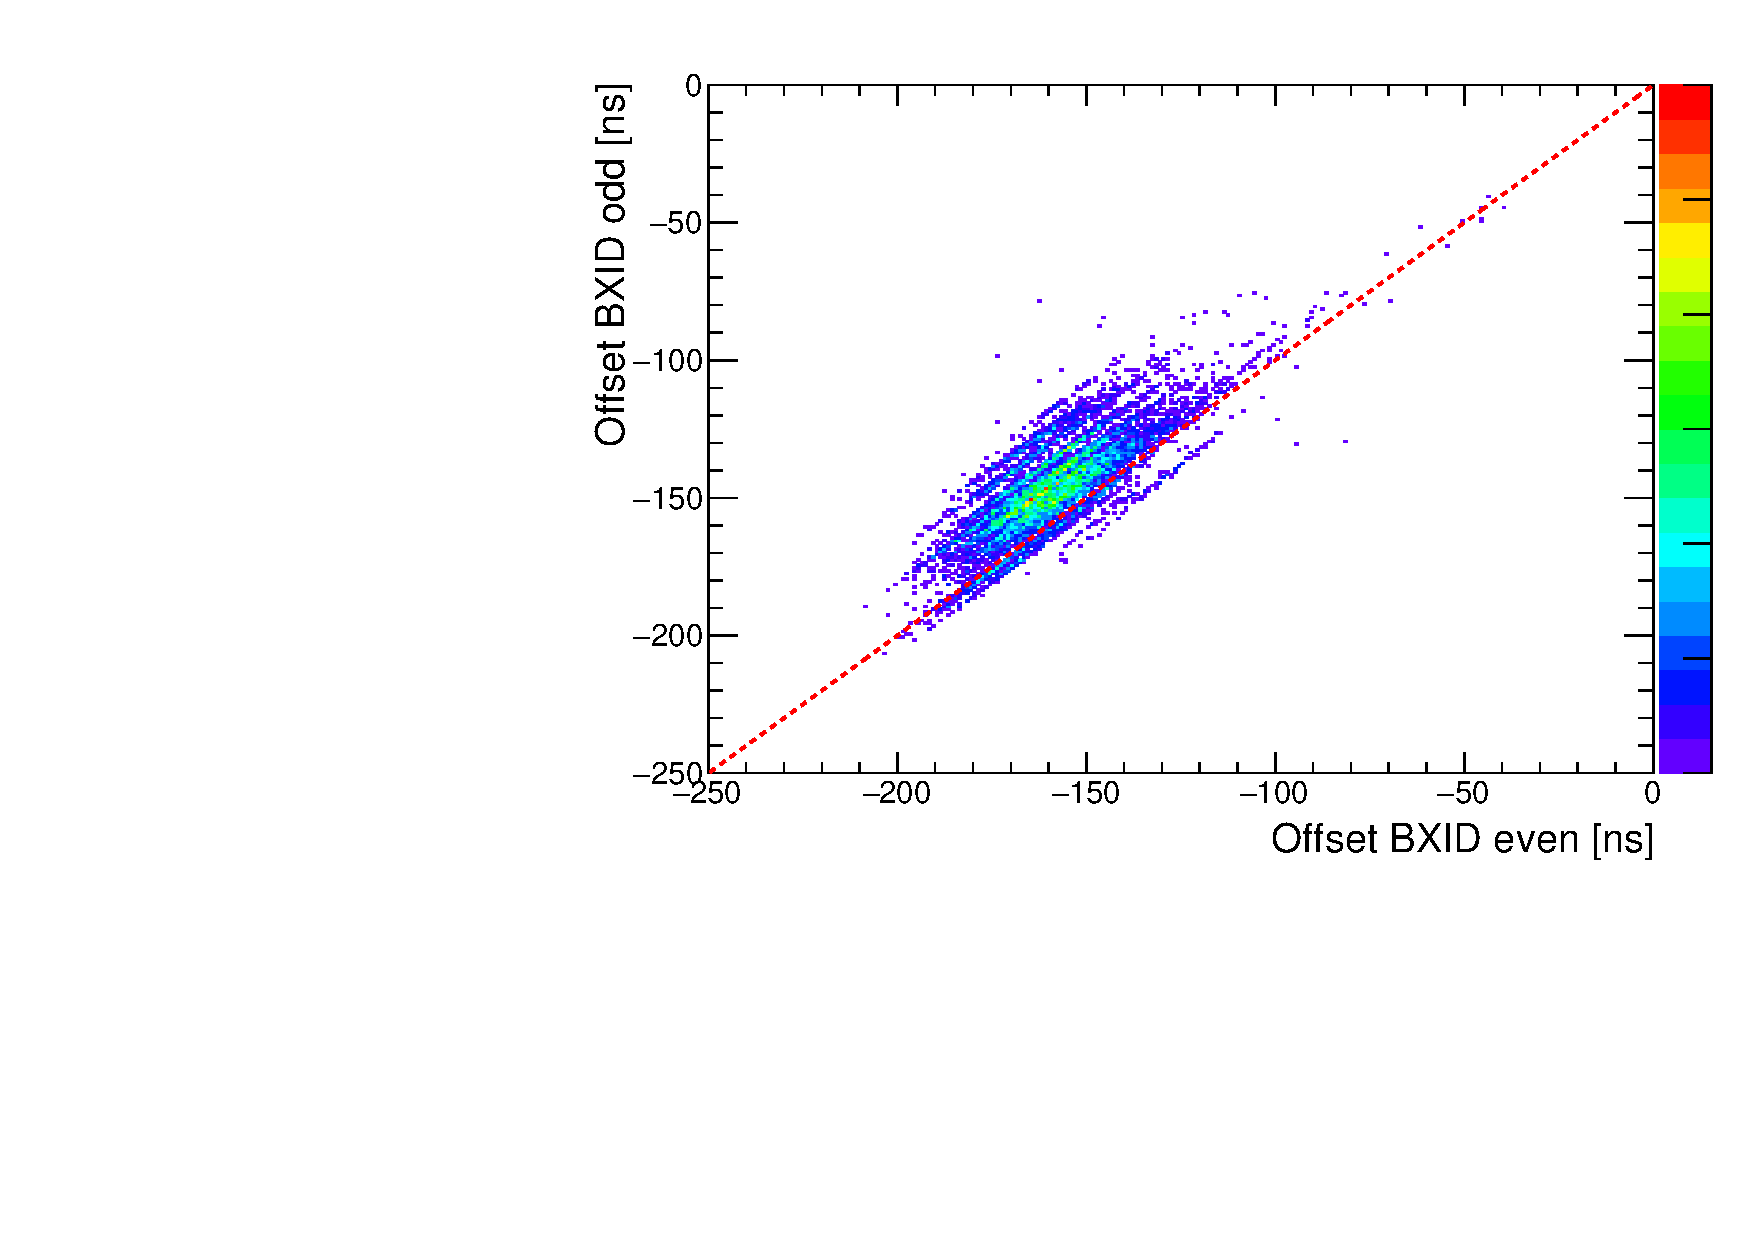
\includegraphics[width=1\textwidth]{../Thesis_Plots/Timing/Muons/Plots/CorrelationOffsets_BXID.pdf}
		\caption{Correlation between offsets extracted for even and odd BXID.}\label{fig:BXID_offset}
	\end{subfigure}
	\caption{\subref{fig:offset_trigger_distribution}) Extracted offset used to correct for the trigger delay signal. The mean delay of the trigger is $\sim$ 150 ns and is in the expected order. \subref{fig:BXID_offset}) Correlation between offsets extracted for BXID even and odd.}
\end{figure}

\subsection{Time of the first hit distribution}

After the selection and calibration, the time of the first hit (T$_{fH}$) can be obtained by plotting the distribution of T$_{chn}$ - T$_{ref}$ as shown in figure \ref{fig:timing_nocorrection}. The time resolution (RMS) shown in figure \ref{fig:timing_nocorrection} obtained by combining all layers excluding layer 11 is around 5.65 ns by just applying the time calibration on the data. This is far from the desired time resolution of 1 ns. Some improvements are still possible as described in the following. An asymmetry can be seen in the time distribution to the left. It is likely coming from the non-linearity of the TDC ramp as explained in the next subsection.

Each layer was also looked at individually as shown in figure \ref{fig:reso_nocorrection}. A comparison between a gaussian fit to extract the $\sigma$ and the RMS of the distribution is done. All layers are very similar in terms of time resolution and gaussian-like. The layer 6 and 10 present a higher time resolution that may be due to the bad quality and low number of working channels of these layers. The discrepancy observed for the layer 11 is most likely due to an electronic problem in the TDC voltage ramp of all the chips on that layer. But the reason is not totally clear and identified.

\begin{figure}[htbp!]
	\begin{subfigure}[t]{0.5\textwidth}
		\centering
		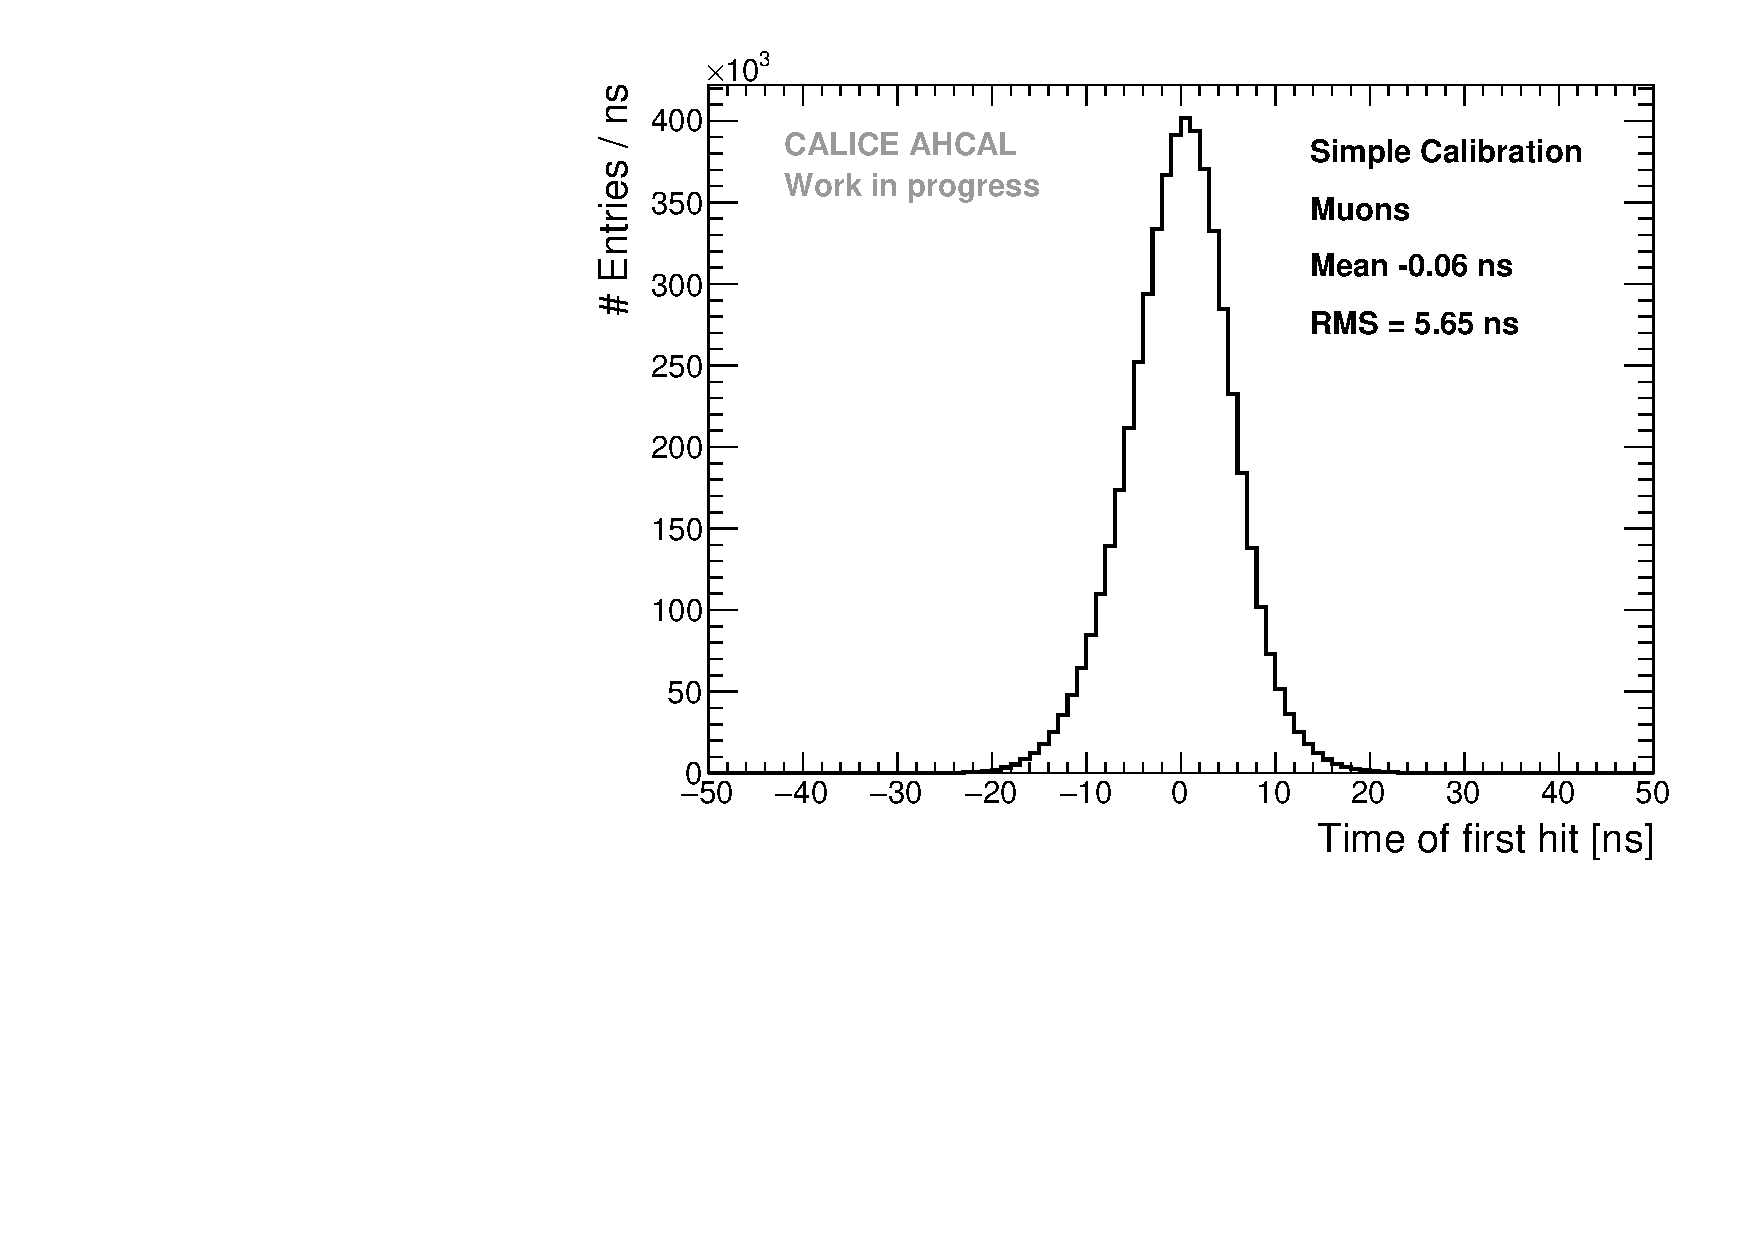
\includegraphics[width=1\textwidth]{../Thesis_Plots/Timing/Muons/Plots/Timing_AHCAL_noCorrections.pdf}
		\caption{Timing for all layers in the AHCAL excluding layer 11.}\label{fig:timing_nocorrection}
	\end{subfigure}
	\hfill
	\begin{subfigure}[t]{0.5\textwidth}
		\centering
		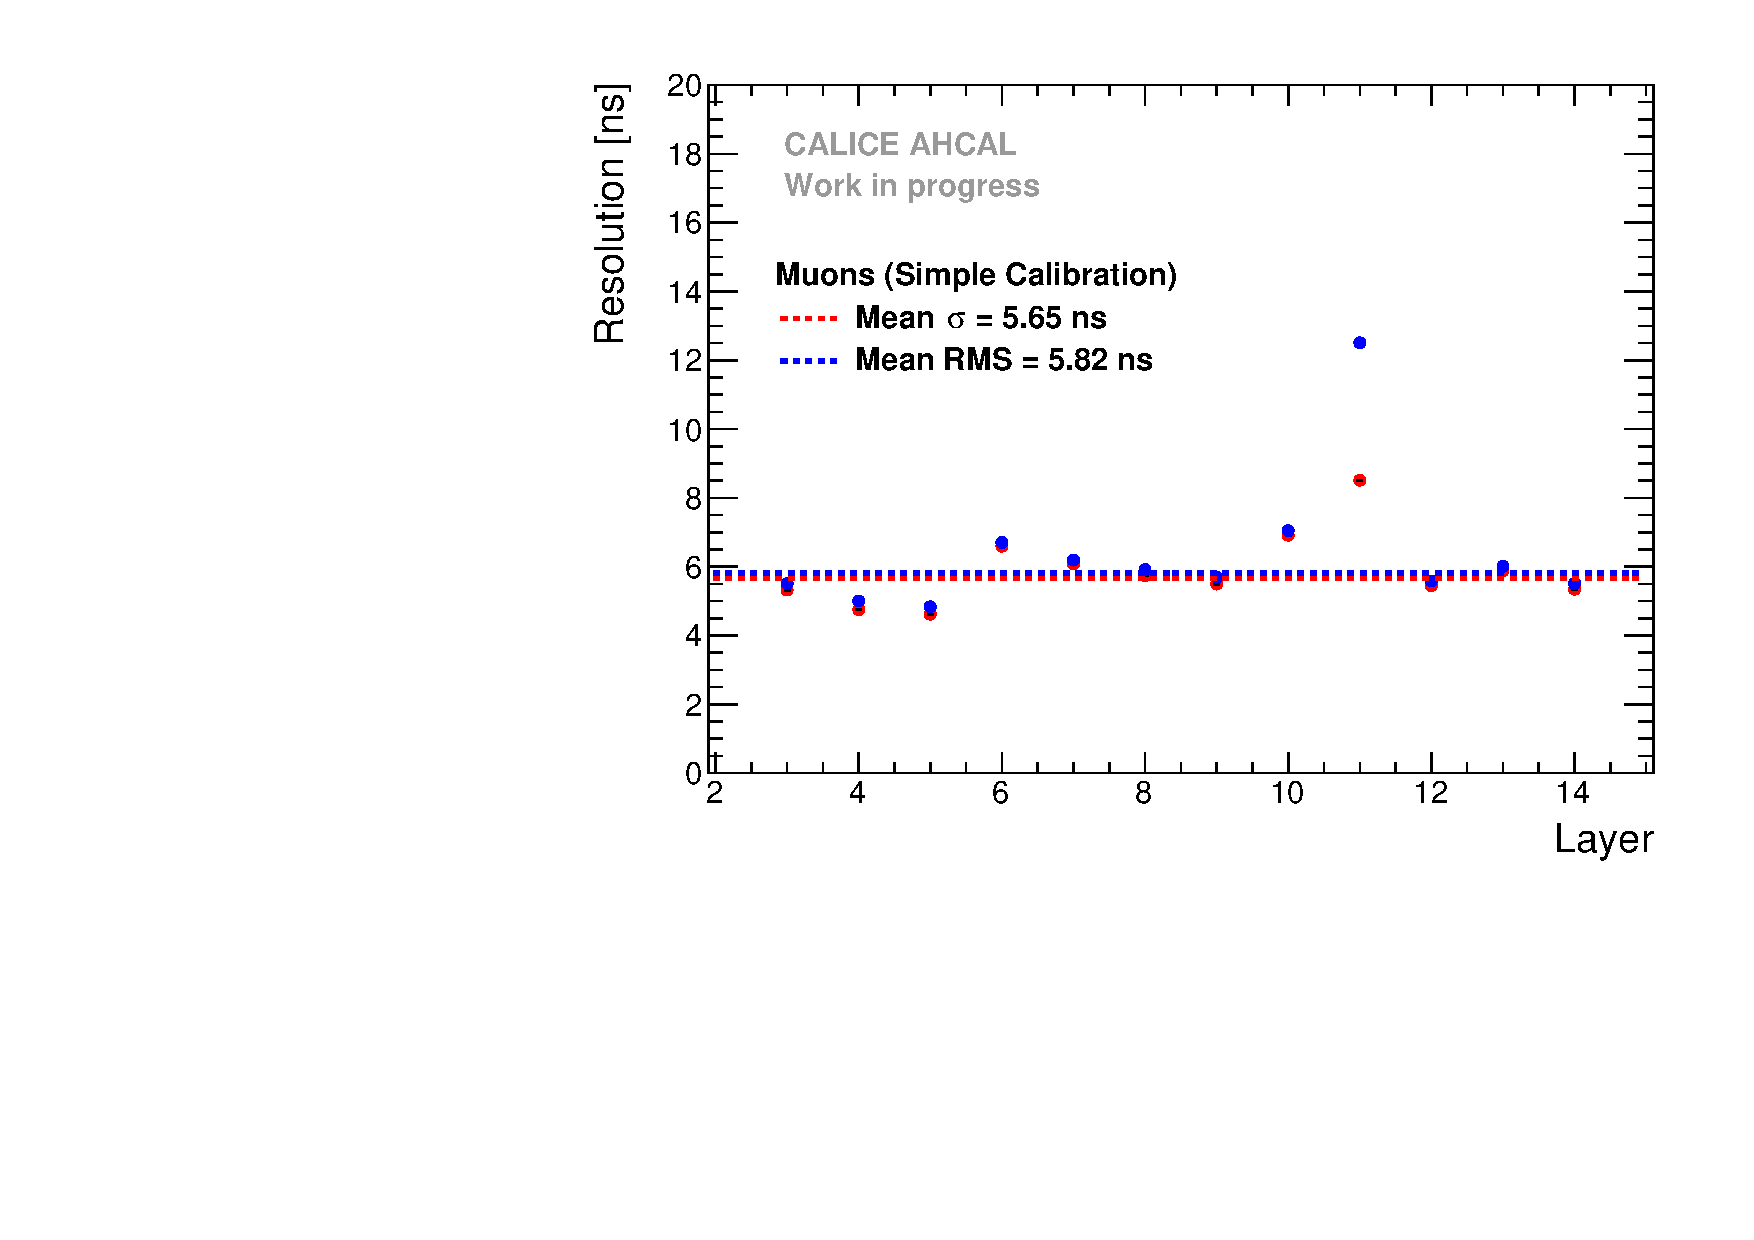
\includegraphics[width=1\textwidth]{../Thesis_Plots/Timing/Muons/Plots/ResolutionPerModule_noCorrections.pdf}
		\caption{Extracted resolution for all layers in the AHCAL.}\label{fig:reso_nocorrection}
	\end{subfigure}
	\caption{\subref{fig:timing_nocorrection}) Time of the first hit distribution of the AHCAL after the first part of the calibration. $\mu$ = -0.06 ns , RMS = 5.65 ns. The distribution is clearly asymmetric to the left. \subref{fig:reso_nocorrection}) Time resolution for all layers in the AHCAL. The mean RMS time resolution is represented by the blue line. Mean $\sigma$ = 5.65 ns, Mean RMS = 5.82 ns.}
\end{figure}

\section{Corrections applied to data}

\subsection{Ramp non-linearity correction}
\label{subsec:lin_corr}

The calibration relies on the linearity of the TDC voltage ramp in the \textit{SPIROC2B} by measuring the minimum and maximum of the ramp and interpolating the slope assuming a linear ramp. This assumption is not entirely reliable as described in \cite{Hartbrich2011, Brianne2012}. The voltage slope shows a slight kink around the middle leading to a non-linear ramp. For this, a correction of the non-linearity is applied. Since also the time reference is determined from a ramp with a kink and can't be corrected due to the lack of external time reference, the position of $T_{ref}$ and $T_{hit}$ on the ramp is actually corrected here.

\begin{figure}[htbp!]
	\begin{subfigure}[t]{0.5\textwidth}
		\centering
		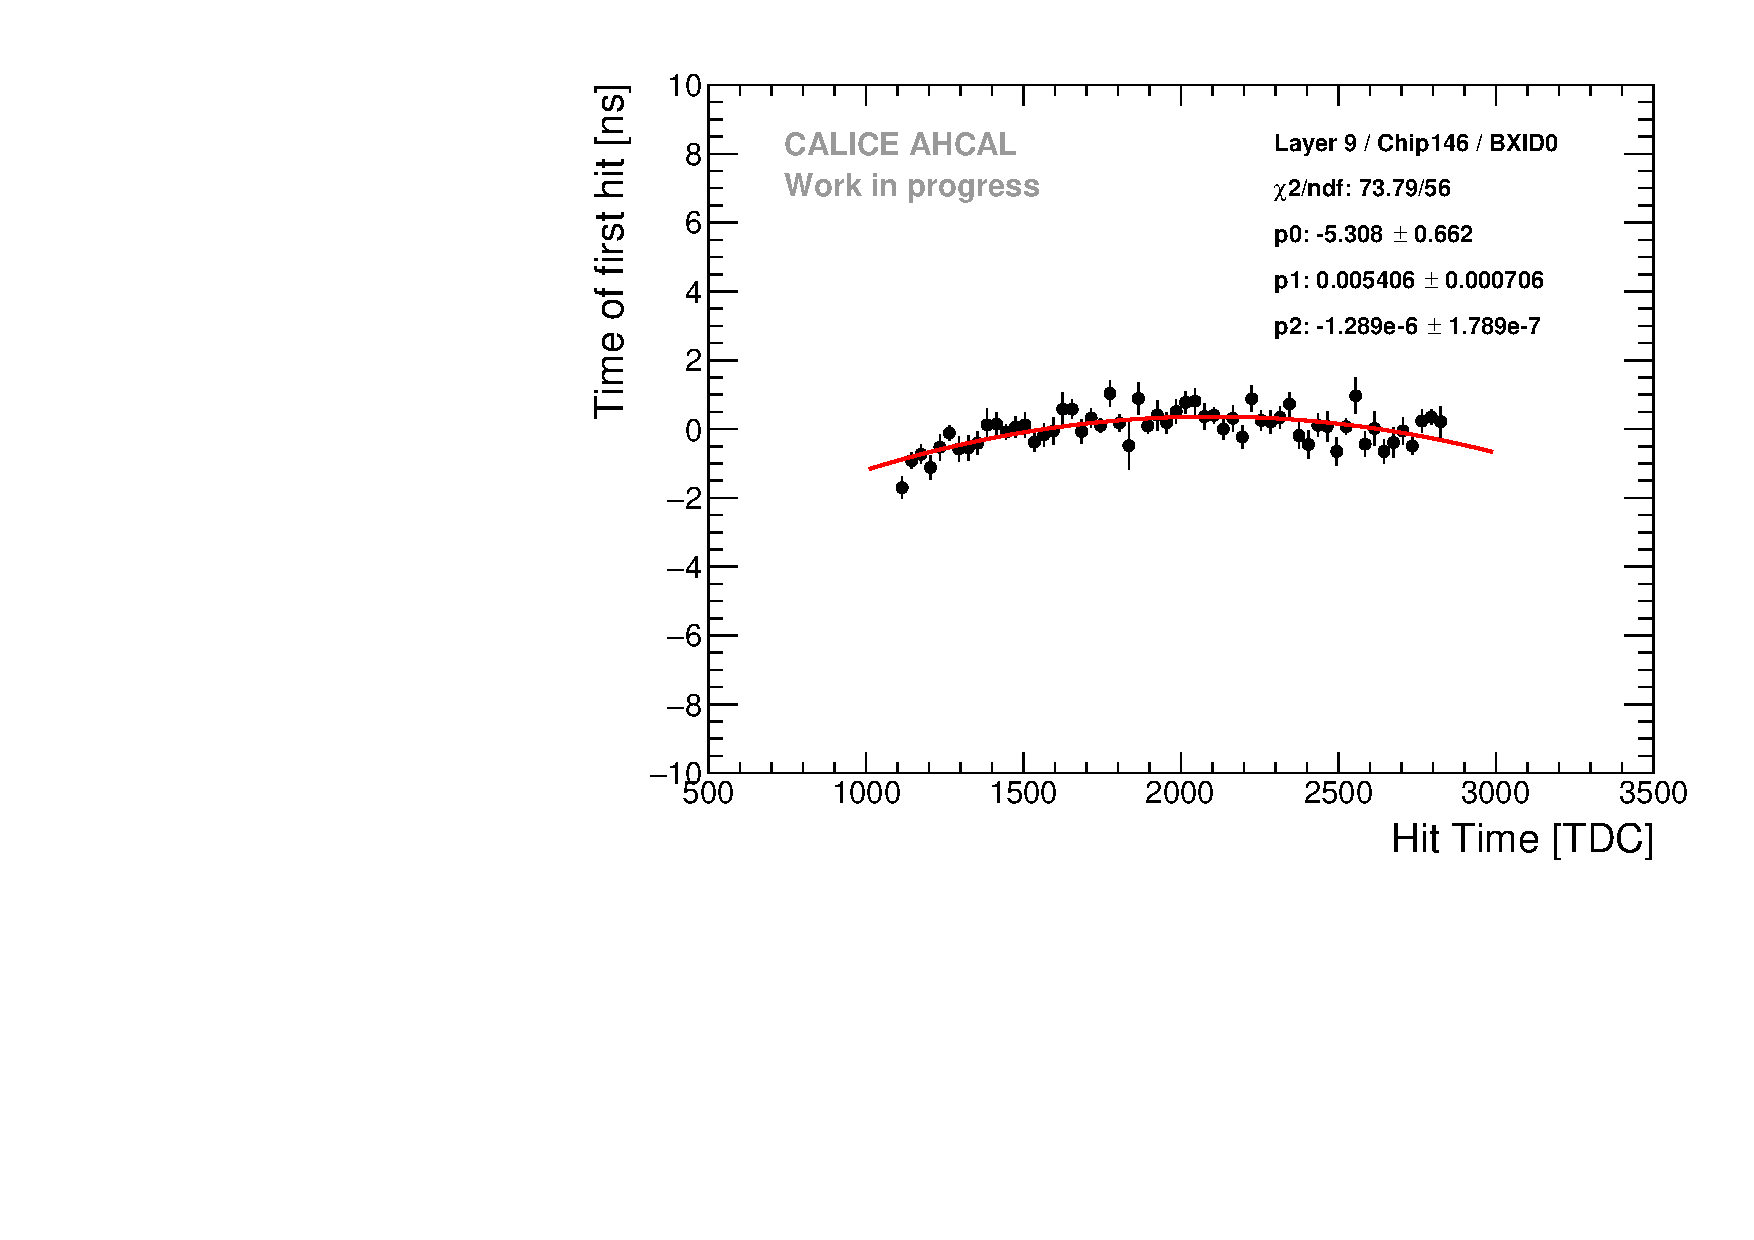
\includegraphics[width=1\textwidth]{../Thesis_Plots/Timing/Muons/Plots/LinearityCorrection_Module09_Chip146_BXID0.pdf}
		\caption{Quadratic fit of chip 146 (BXID even) on layer 9.}\label{fig:LinCorr}
	\end{subfigure}
	\hfill
	\begin{subfigure}[t]{0.5\textwidth}
		\centering
		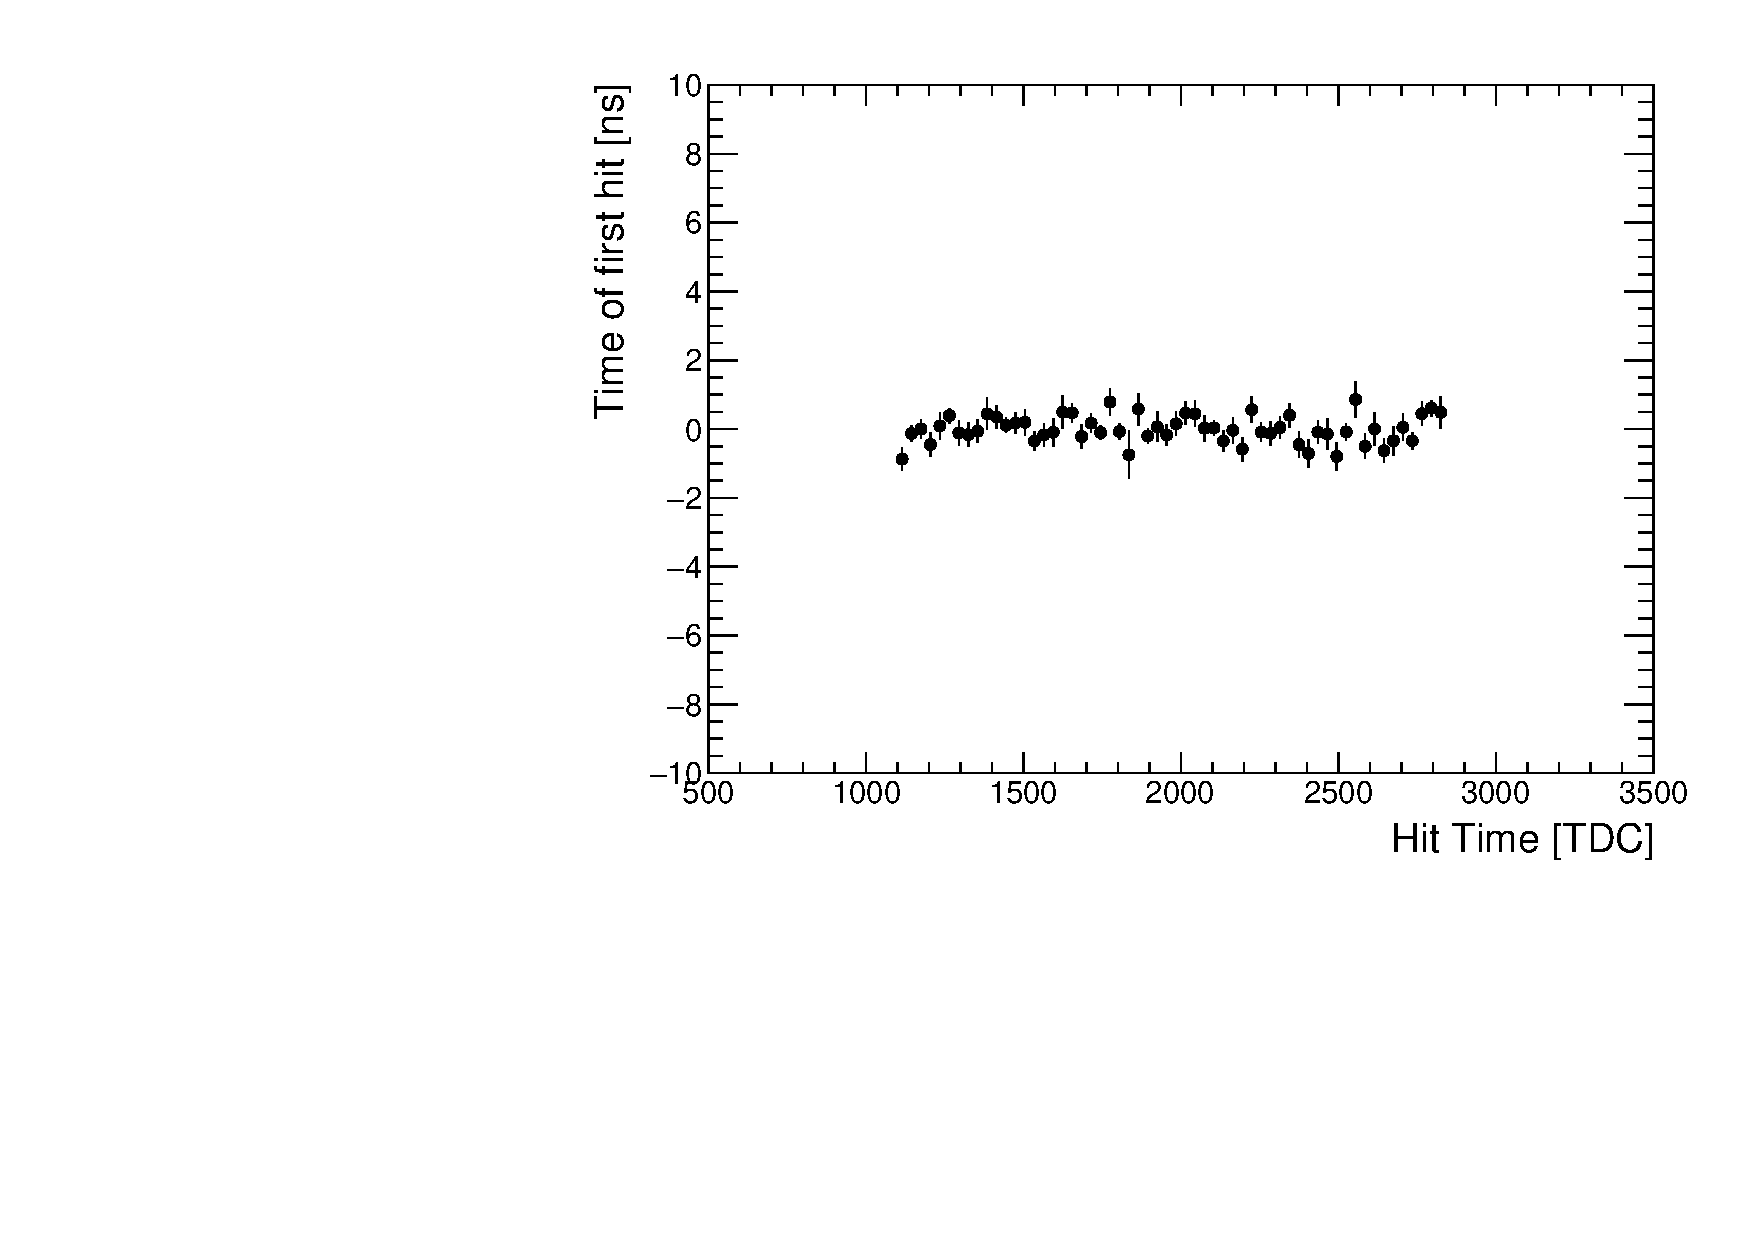
\includegraphics[width=1\textwidth]{../Thesis_Plots/Timing/Muons/Plots/LinearityCorrection_Module09_Chip146_BXID0_Corrected.pdf}
		\caption{Profile for chip 146 on layer 9 after the non-linearity correction of the ramp.}\label{fig:LinCorr_2}
	\end{subfigure}
	\caption{\subref{fig:LinCorr}) Typical profile of the time of the hit versus the TDC of the hit before the non-linearity correction. The graph is slightly curved showing that this chip presents a non-linear TDC ramp. The $\chi^2/ndf$ of the fit is 1.29. \subref{fig:LinCorr_2}) The correction parameters are applied then on the data to cross-check the quality of the correction. One can see that the curve flattens with the correction applied.}
\end{figure}

By looking at the time of the first hit (T$_{fH}$) for each chip and BXID versus the TDC value of the hit, the shape of the graph indicates how reliable is the assumption of a linear ramp. If the ramp would be perfectly linear, one would obtain a flat graph. To correct for the non-linearity of the ramp, a quadratic fit is performed for each chip and BXID as shown in figure \ref{fig:LinCorr}. The correction needed can be in the order of few nanoseconds. The figure \ref{fig:LinCorr_2} shows the time of first hit as a function of the TDC value of the hit after the correction, the graph looks much flatter.

The non-linearity correction results in an improvement in the timing resolution (RMS) of the AHCAL of about 5.1\% (from 5.65 to 5.36 ns) as shown in figure \ref{fig:timing_lincorrection}. The asymmetry of the time distribution remains and is most likely due to the time reference which is non corrected for the non-linearity as no external time reference for these channels is present. Looking at each layer, as shown on figure \ref{fig:reso_lincorrection}, the time resolution went down by the same amount.

\begin{figure}[htbp!]
	\begin{subfigure}[t]{0.5\textwidth}
		\centering
		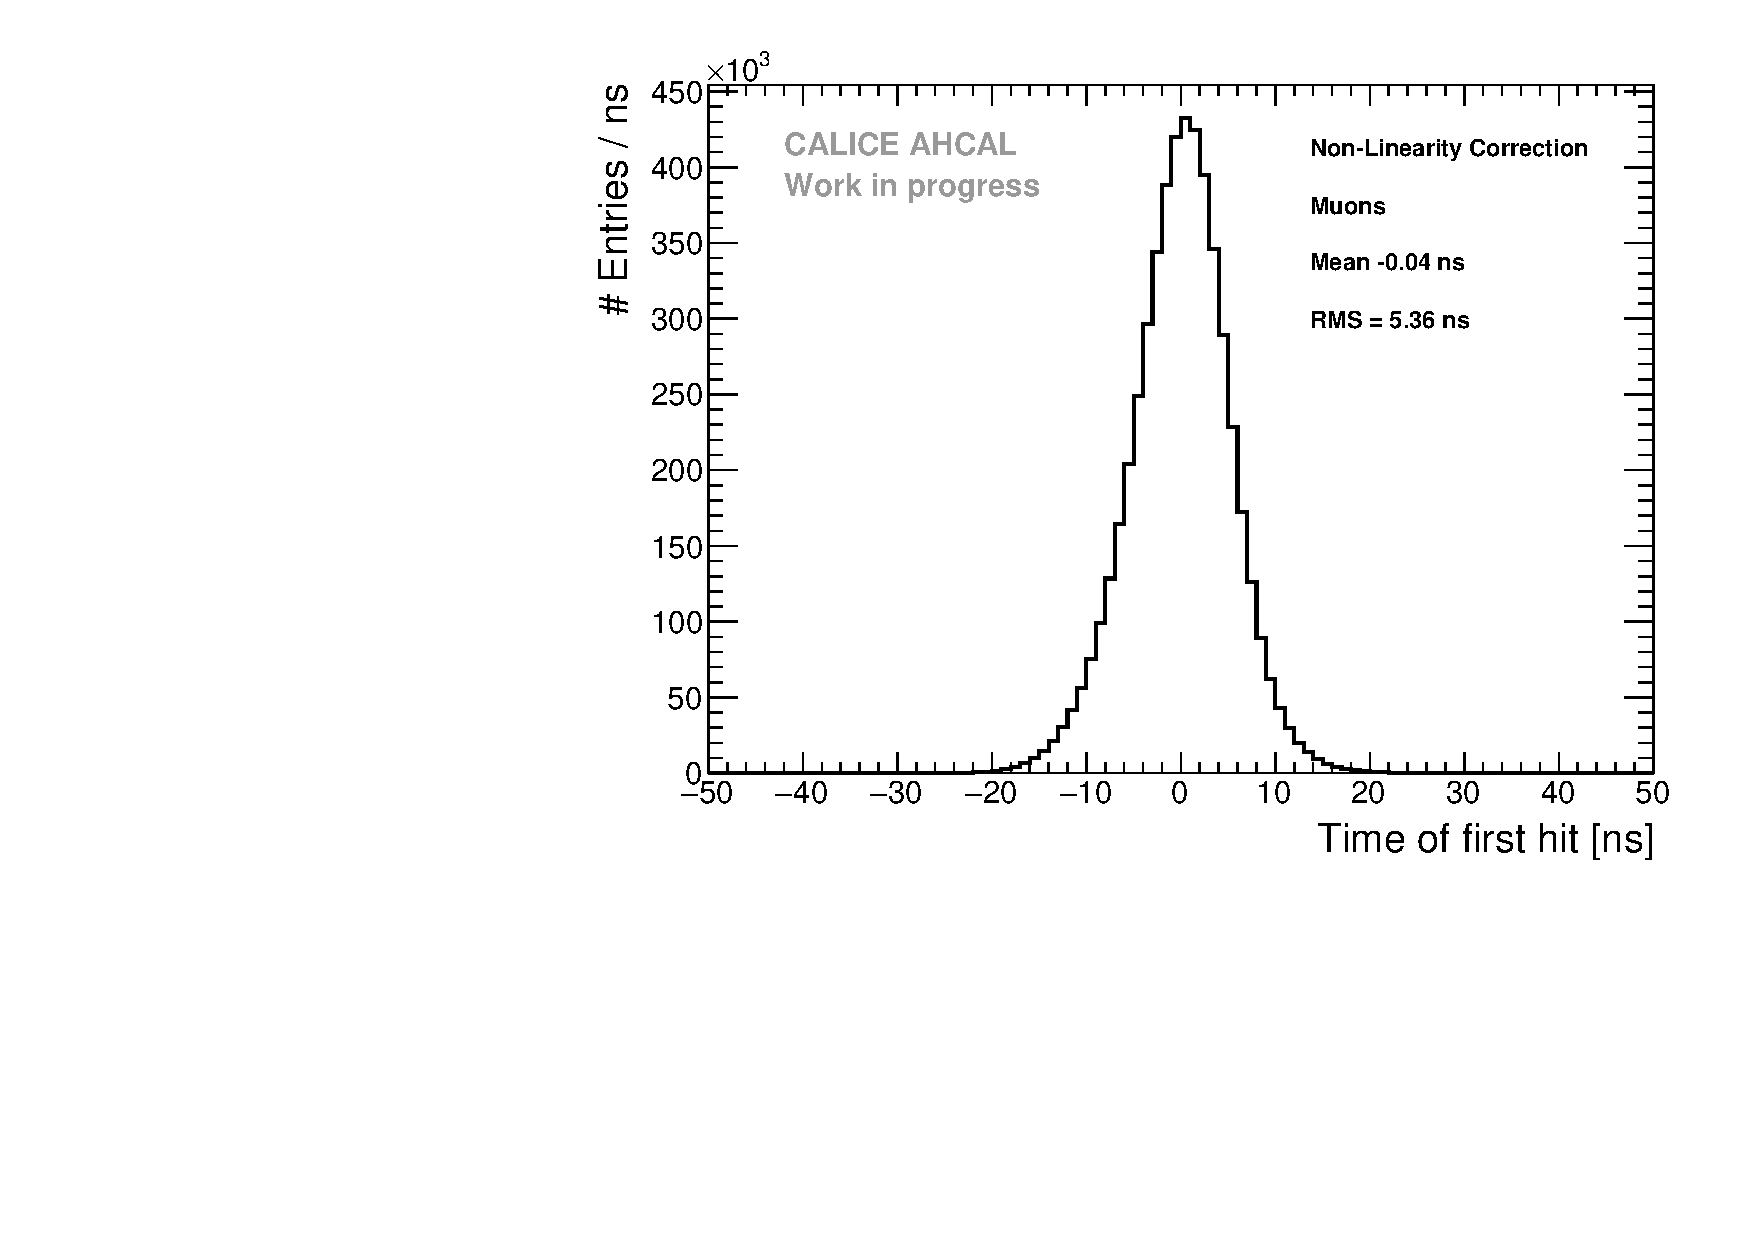
\includegraphics[width=1\textwidth]{../Thesis_Plots/Timing/Muons/Plots/Timing_AHCAL_LinCorrection.pdf}
		\caption{Timing for all layers in the AHCAL excluding layer 11.}\label{fig:timing_lincorrection}
	\end{subfigure}
	\hfill
	\begin{subfigure}[t]{0.5\textwidth}
		\centering
		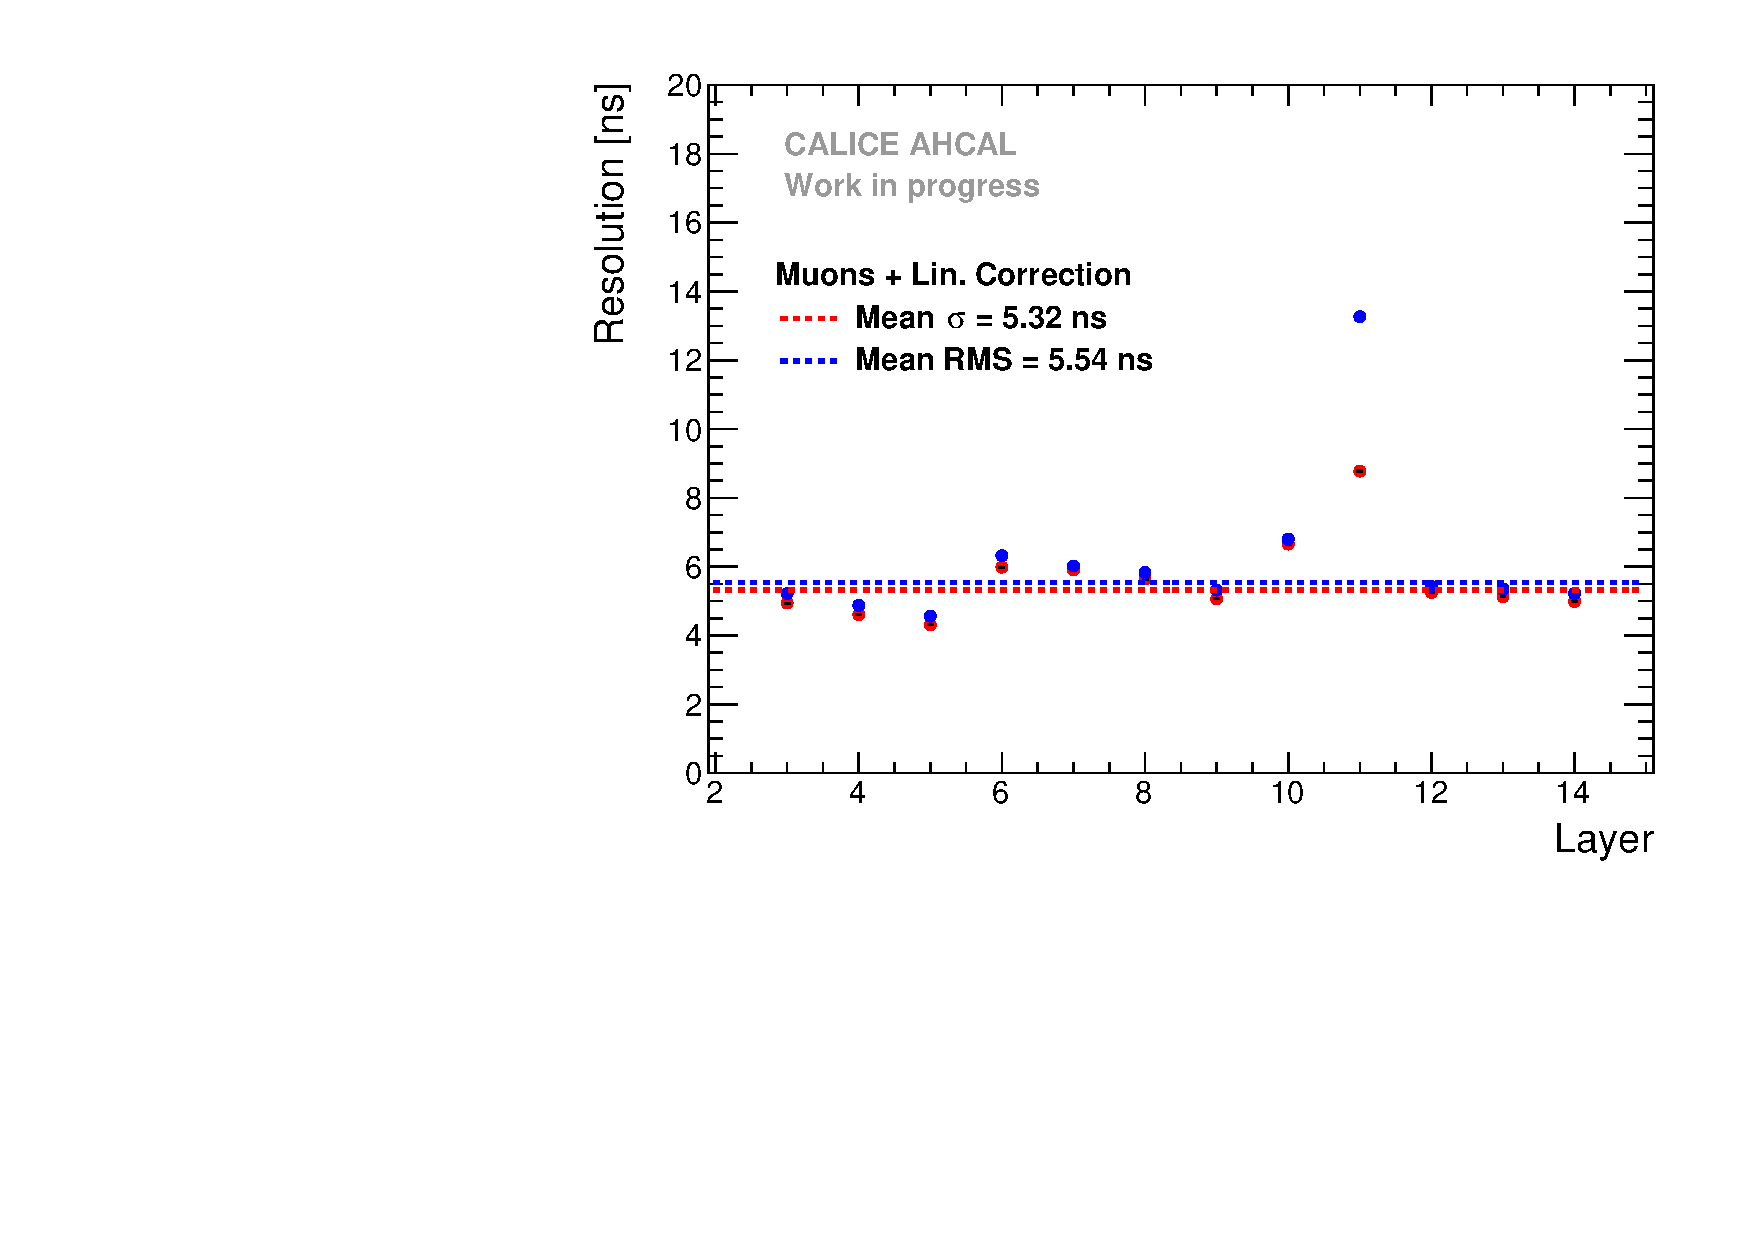
\includegraphics[width=1\textwidth]{../Thesis_Plots/Timing/Muons/Plots/ResolutionPerModule_LinCorrection.pdf}
		\caption{Extracted resolution for all layers in the AHCAL.}\label{fig:reso_lincorrection}
	\end{subfigure}
	\caption{\subref{fig:timing_lincorrection}) Time of the first hit distribution of the AHCAL after the non-linearity correction. $\mu$ = -0.04 ns , RMS = 5.36 ns. \subref{fig:reso_lincorrection}) Time resolution for all layers in the AHCAL. The mean RMS is 5.54 ns.}
\end{figure}

\subsection{Time Walk correction}
\label{subsec:timewalk}

The time-walk effect is due to the presence of a threshold that induces a time shift between a small amplitude signal and a high amplitude signal. Small amplitude signals will systematically trigger at a later time than high amplitude signals. A correction can be applied on the data by looking at the time of the first hit versus the amplitude of the hit. This might be particularly important for late neutrons signals that generally deposit very little energy in the calorimeter.

The correction is assumed to be the same for all the chips, independent of the position of the threshold of each chip, as hits are cut at 0.5 MIP. Thresholds of most of the chips were set to similar values and the threshold was set-up well below 0.5 MIP. An exponential fit of the form $\text{A} \times e^{-\lambda{}x} + \text{B}$ is performed on the data to extract the parameters needed to correct the time walk effect as shown on figure \ref{fig:time_walk}. The residuals after correction are in the order of few hundreds of picoseconds as seen in figure \ref{fig:time_walk_corr}.

\begin{figure}[htbp!]
	\begin{subfigure}[t]{0.5\textwidth}
		\centering
		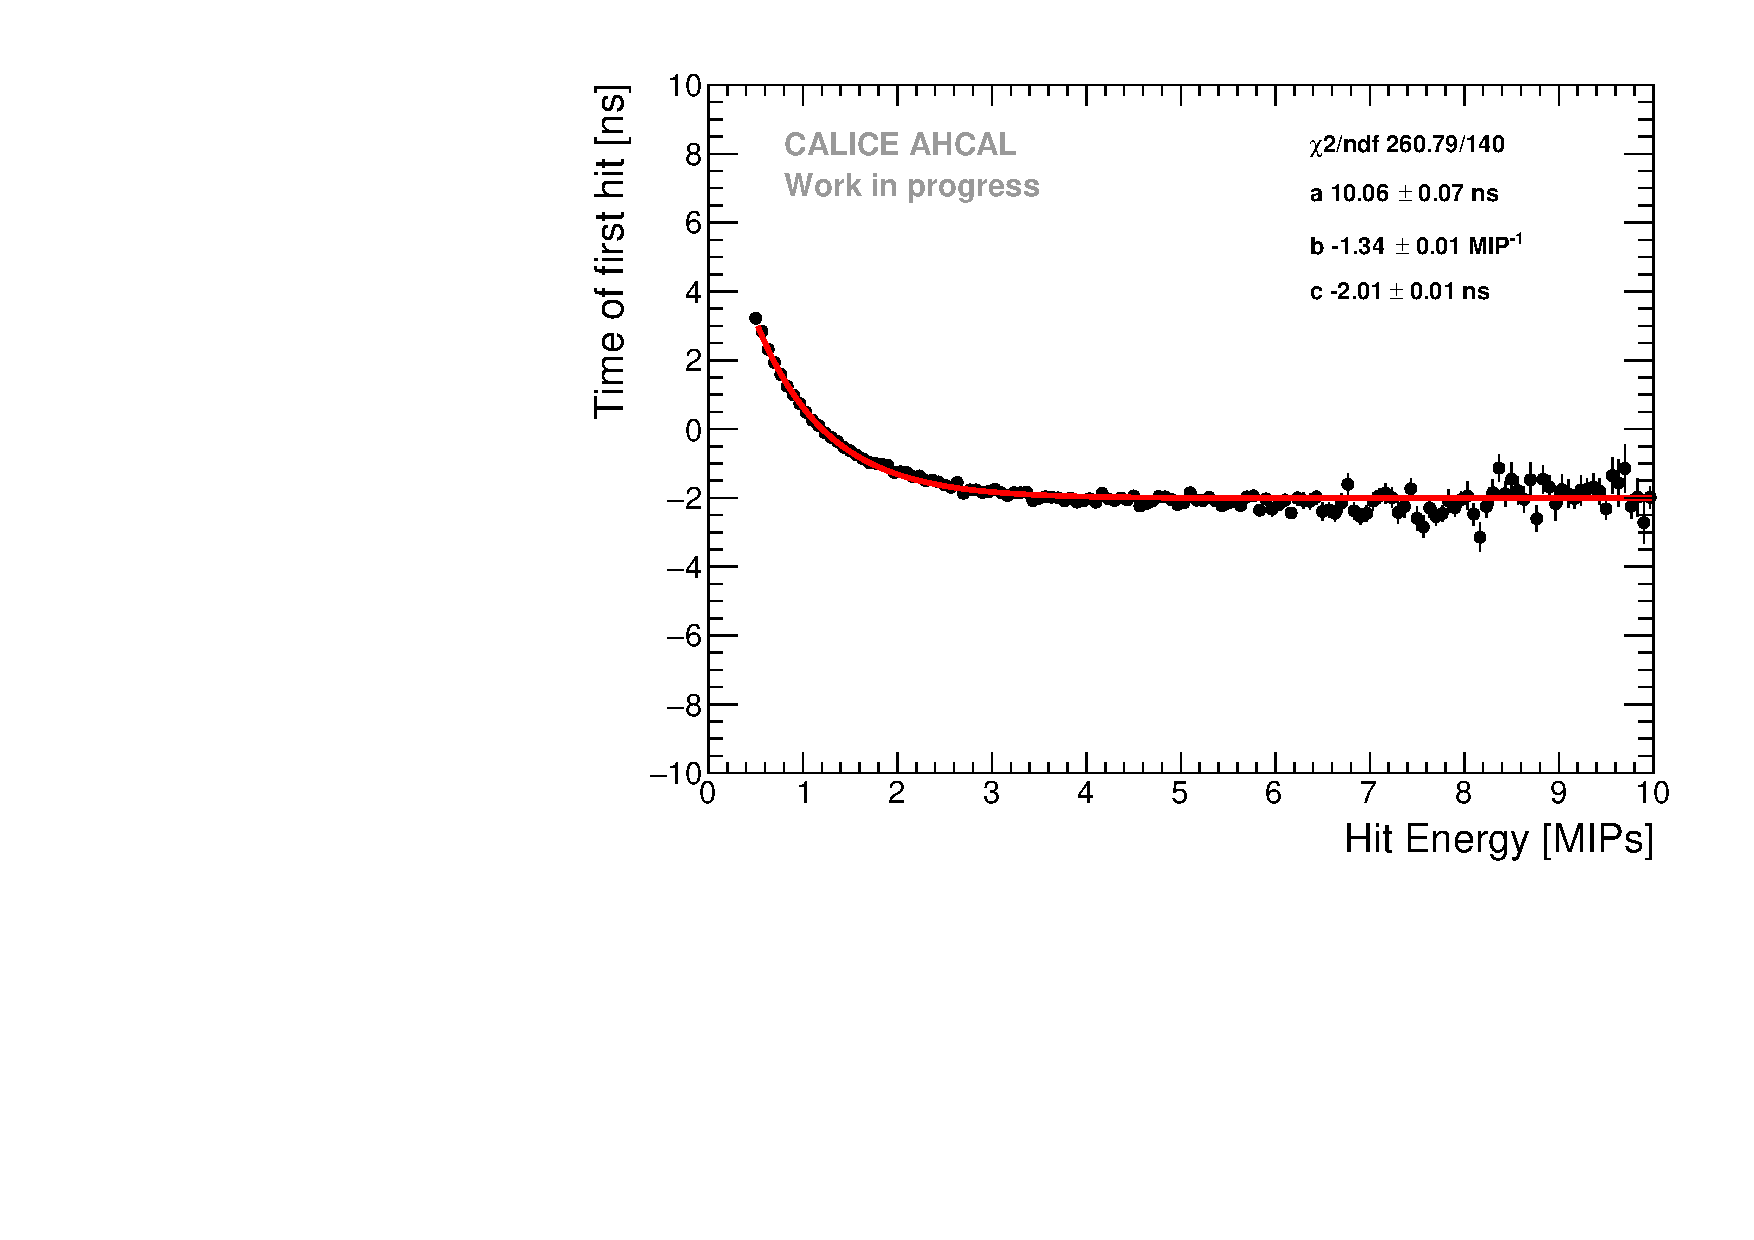
\includegraphics[width=1\textwidth]{../Thesis_Plots/Timing/Muons/Plots/TimeWalkProfile.pdf}
		\caption{Profile of the time of first hit as function of the hit energy.}\label{fig:time_walk}
	\end{subfigure}
	\hfill
	\begin{subfigure}[t]{0.5\textwidth}
		\centering
		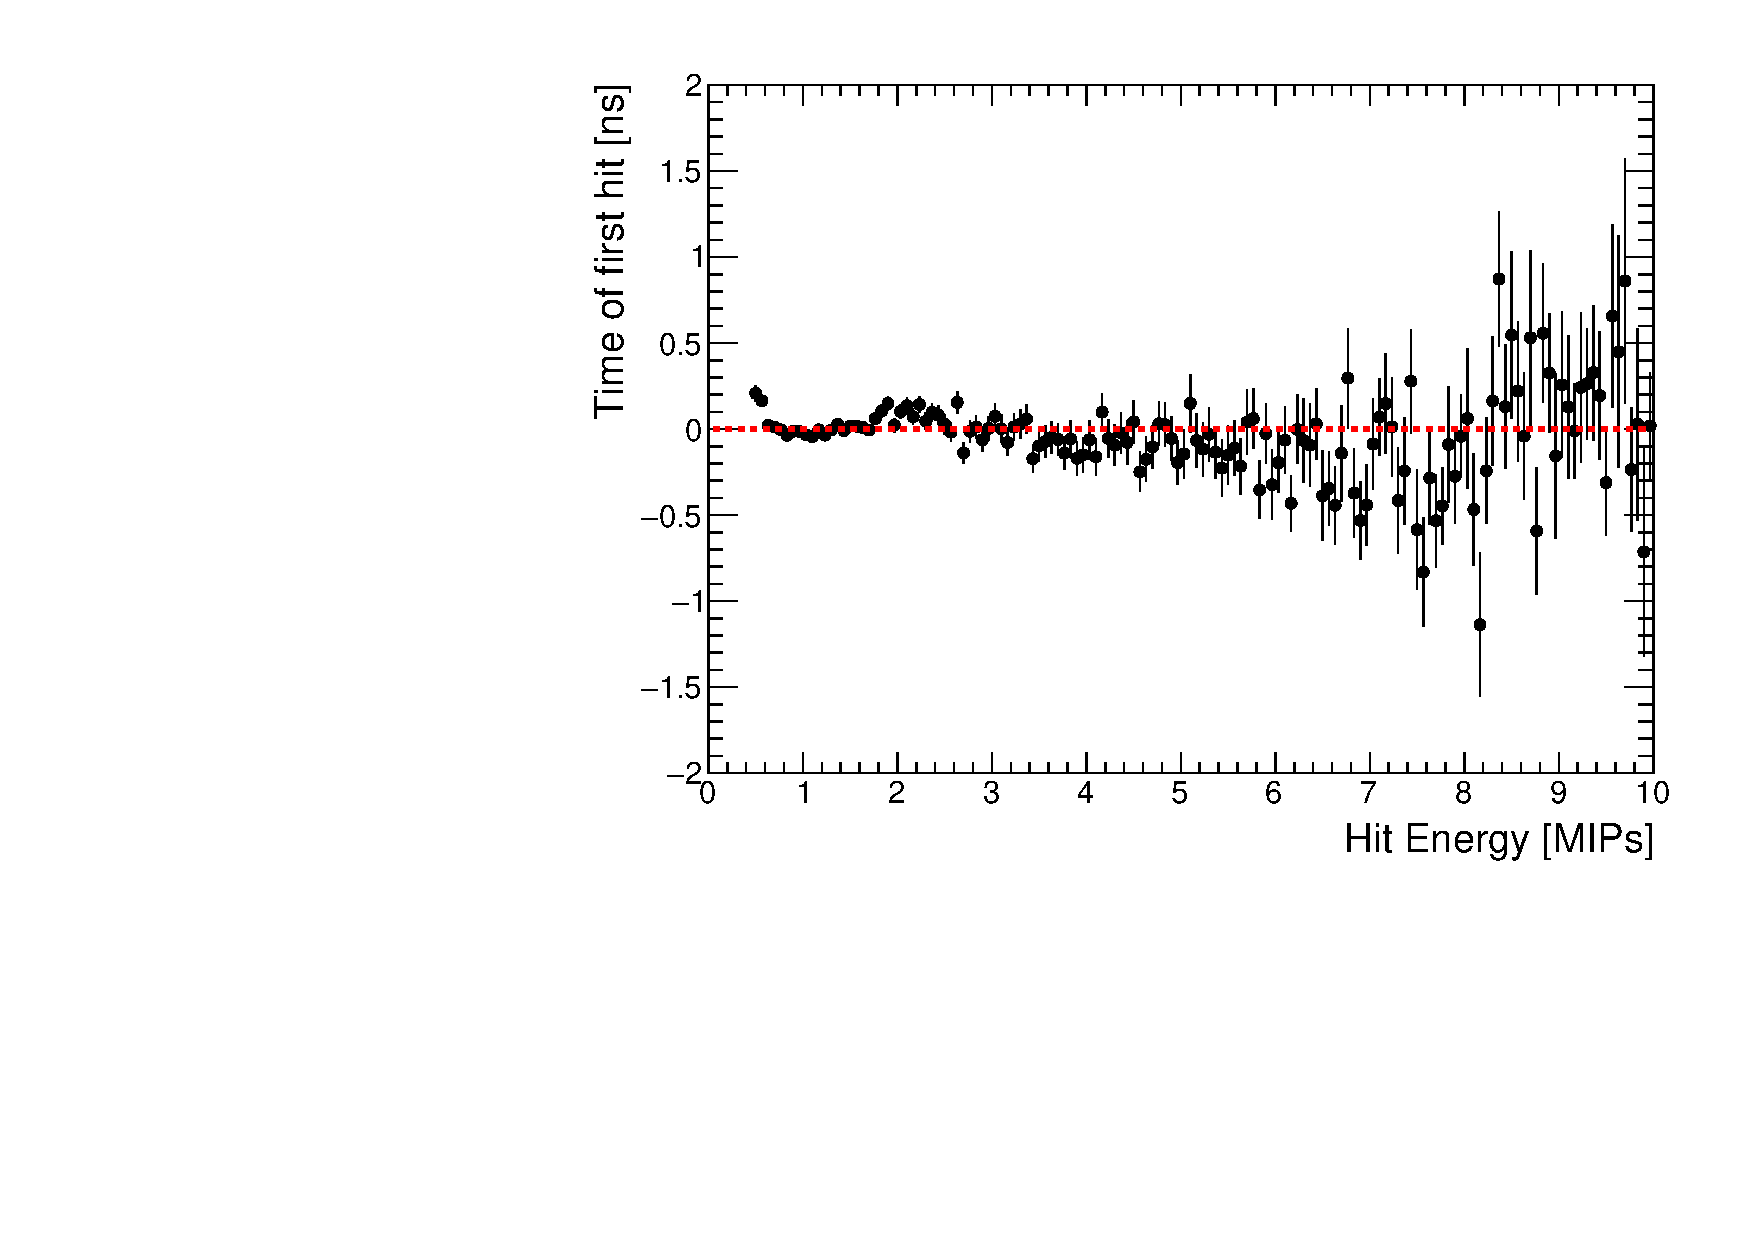
\includegraphics[width=1\textwidth]{../Thesis_Plots/Timing/Muons/Plots/TimeWalkProfile_Correction.pdf}
		\caption{Same profile after time-walk correction.}\label{fig:time_walk_corr}
	\end{subfigure}
	\caption{\subref{fig:time_walk}) Time-walk correction extracted from data. A = 10.06 $\pm$ 0.07, $\lambda$ = -1.34 $\pm$ 0.01, B = -2.01 $\pm$ 0.01. A difference up to 6 ns is seen between small and large amplitudes. \subref{fig:time_walk_corr}) Time-walk profile after correction showing a spread of less than 1 ns.}
\end{figure}

\subsection{Time of first hit for muons after corrections}
\label{subsec:Muon_final}

After the time-walk correction, an improvement of around 3\% can be achieved on the time resolution of the AHCAL as shown in figure \ref{fig:timing_muons}. The figure \ref{fig:timing_reso_all_muons} shows the time resolution obtained for all the layers in the AHCAL. The obtained time resolution is around 5.2 ns RMS. The distribution is still asymmetric and it is taken into account in the simulation by parametrizing the time distribution with a double Gaussian function (see table \ref{table:time_res_sim}). The number of events identified later than 5$\sigma$ ($\sim$ 25 ns) is around 1.22\% giving a good assessment of the noise suppression for muons.

\begin{figure}[htbp!]
	\begin{subfigure}[t]{0.5\textwidth}
		\centering
		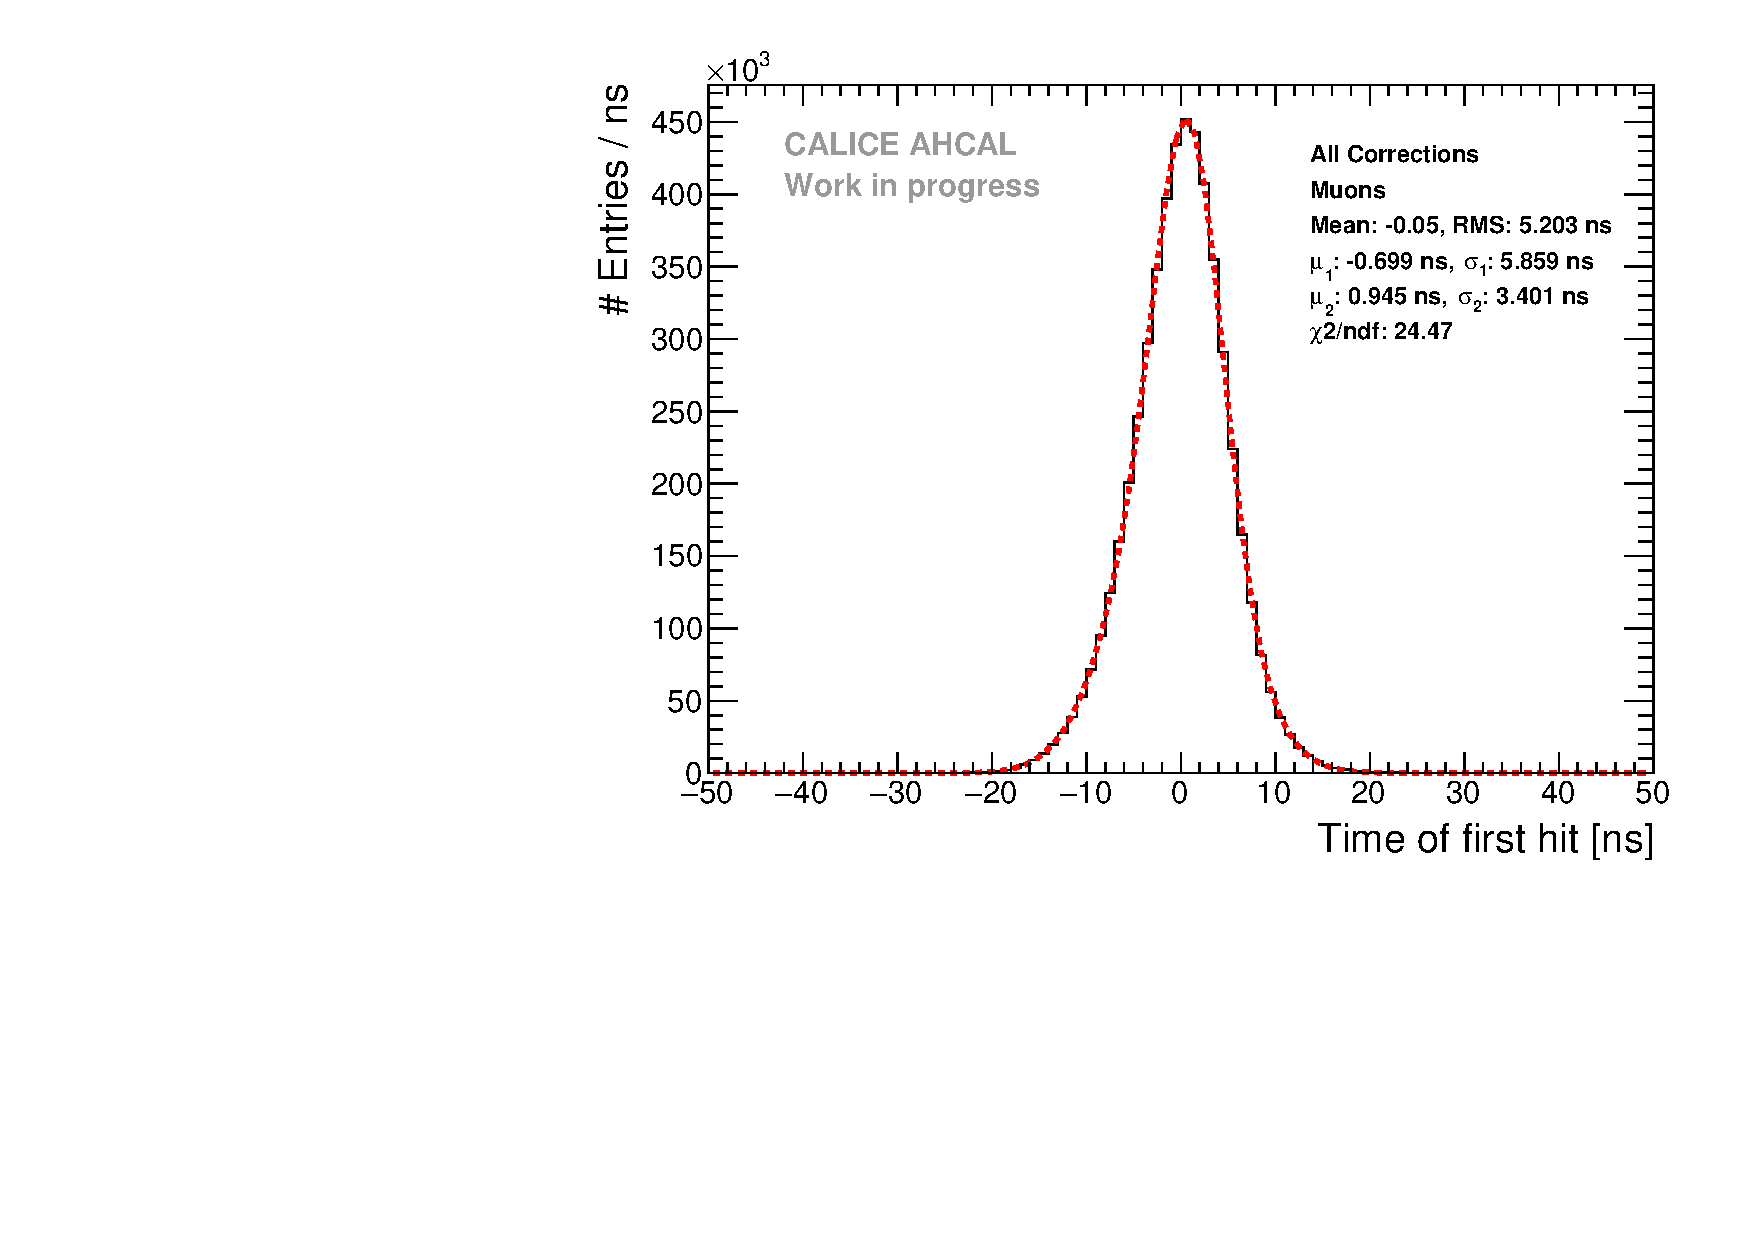
\includegraphics[width=1\textwidth]{../Thesis_Plots/Timing/Muons/Plots/Timing_AllLayers.pdf}
		\caption{Time of the first hit distribution of the AHCAL after all corrections.}\label{fig:timing_muons}
	\end{subfigure}
	\hfill
	\begin{subfigure}[t]{0.5\textwidth}
		\centering
		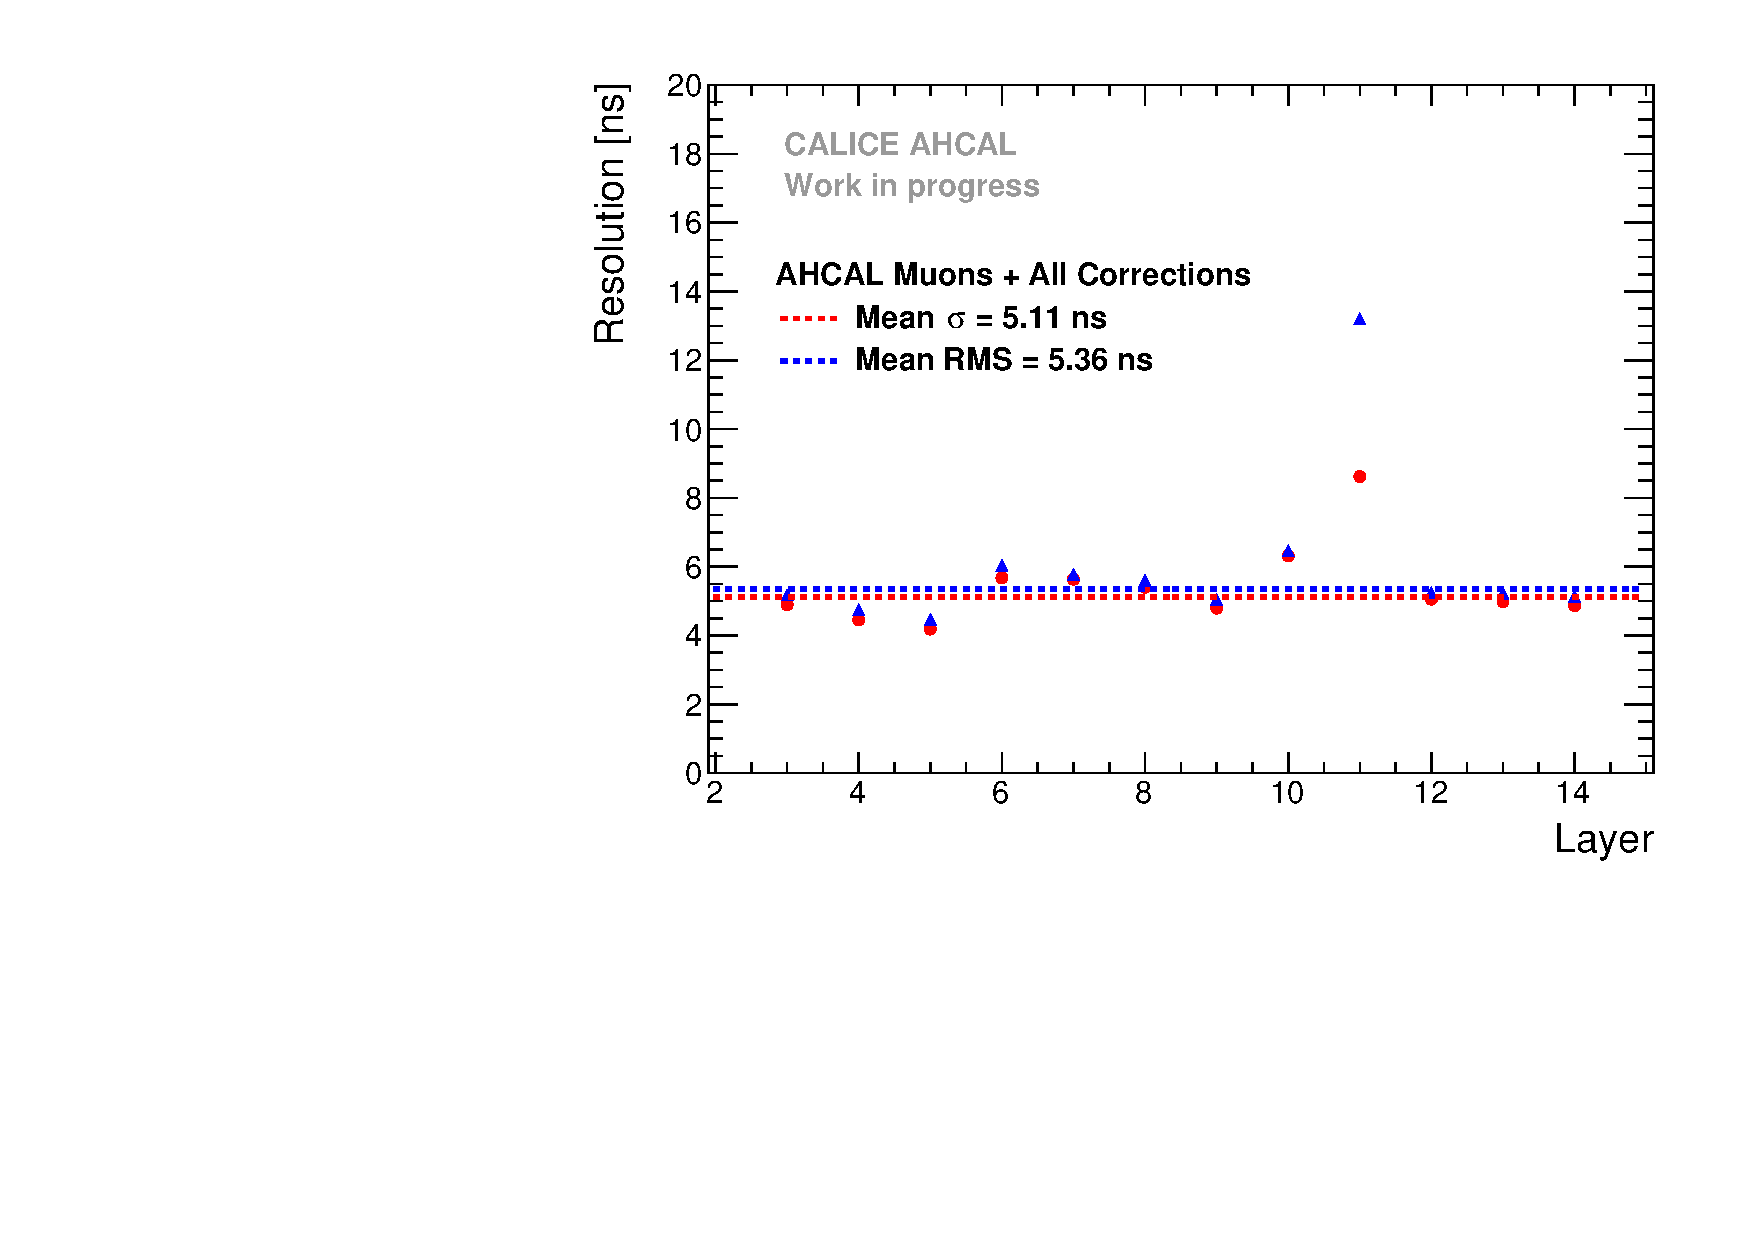
\includegraphics[width=1\textwidth]{../Thesis_Plots/Timing/Muons/Plots/ResolutionPerModule_AllCorrection.pdf}
		\caption{Time resolution obtained for each AHCAL layers.}\label{fig:timing_reso_all_muons}
	\end{subfigure}
	\caption{\subref{fig:timing_muons}) Time of the first hit for muons after all corrections excluding layer 11. The extracted parameters are then used to tune the simulation. \subref{fig:timing_reso_all_muons}) Time resolution obtained for each layer in the AHCAL. Mean RMS = 5.35 ns.}
\end{figure}

After all corrections, the time resolution obtained is far from the 1 ns time resolution desired which is most likely due to the domination in the time resolution of the time reference. Assuming that it is a simple convolution of the time resolution of the AHCAL and the resolution of the time reference, then the AHCAL time resolution would be around $\sigma_{AHCAL} \sim \sqrt{\frac{\sigma_{t}^2 - \sigma_{Tref}^2}{3}} \sim$ 1.91 ns % need to discuss this with Katja %
which is consistent with previous measurements of single channel time resolution \cite{Laurien2016}.

\section{Cross-check of the calibration with electrons}
\label{subsec:validation}

In order to validate the calibration, an electron sample is taken. Electromagnetic showers are quasi-instantaneous and perfect to cross-check the time calibration procedure. The selection applied to the data sample is described in subsection \ref{subsec:elec_sel}. The same calibration constants and correction constants are applied to the data except that an additional offset from the trigger signal has to be corrected for.

The additional offset is expected to be small as the trigger configuration is very similar to the one for muons. The offset is in the order of 10 ns which is consistent with the changes in trigger configuration from the big scintillator plates to the small trigger scintillator of $10\times10$ cm$^2$. The time of the first hit distribution is shown in figure \ref{fig:Timing_electrons}. The time distribution presents a large tail to the right and is much wider than for muons. This gives a hint that an effect is present in electron data but not in muon data. The difference seen could be related to the fact that in electromagnetic showers, the number of hits is much higher as well as the energy deposited in a single cell can be over hundreds MIP.

\begin{figure}[htbp!]
	\centering
	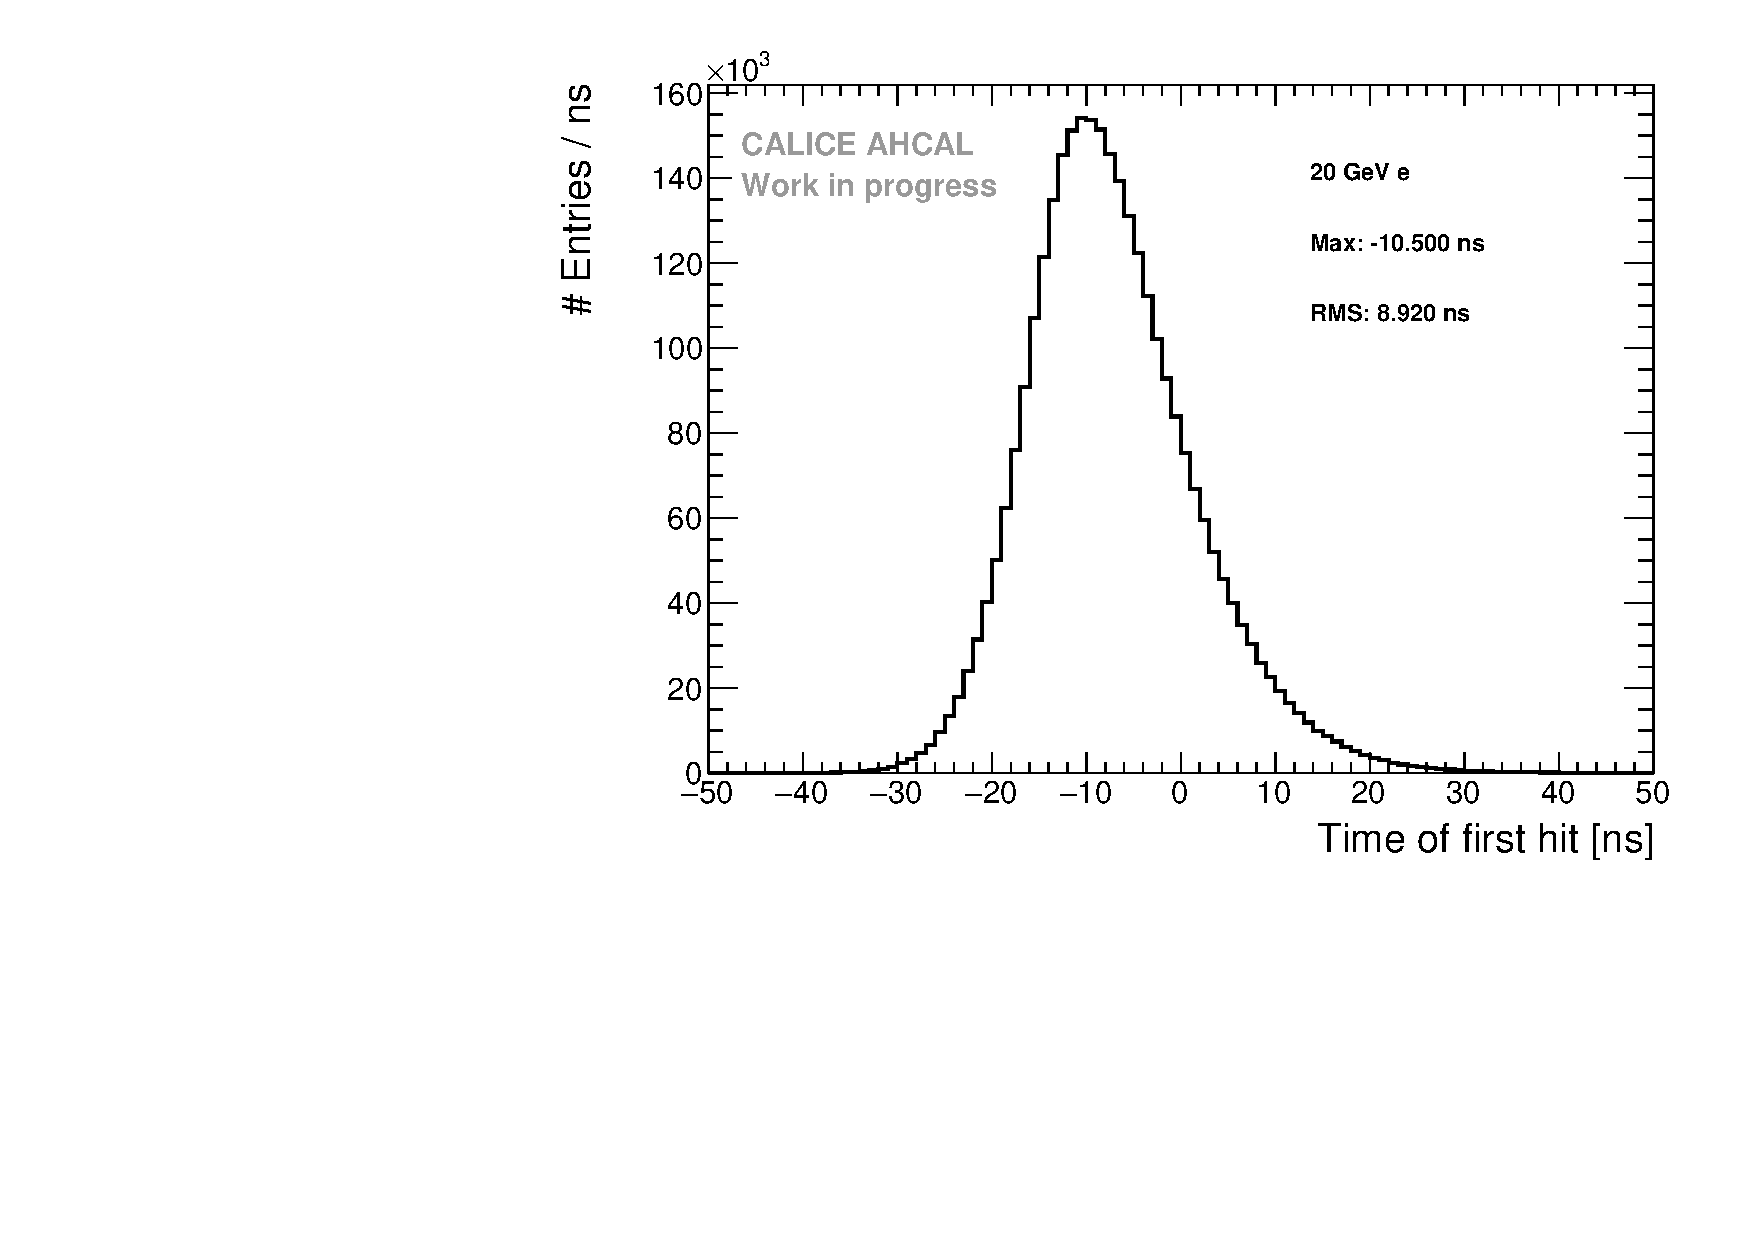
\includegraphics[width=0.6\textwidth]{../Thesis_Plots/Timing/Electrons/Plots/Timing_AllLayers_AfterMuons.pdf}
	\caption{Time of the first hit distribution for 20 GeV electrons after applying the calibration constants extracted from the muon data, before further corrections. Max = -10.05 ns, RMS = 8.92 ns.}
	\label{fig:Timing_electrons}
\end{figure}

\section{Influence of the number of triggered channels}
\label{subsec:ped_shift}

Pedestal shift for energy measurement is not a new feature of the \textit{SPIROC2B} chip \cite{Hartbrich2012}. This electronic effect may be also present for the timing measurement. It can be investigated by looking at the time of the first hit as a function of the number of triggered channels over 0.5 MIP. The correction should not be energy dependent and all electron beam energies are used to determine the correction curve.

It is shown in figure \ref{fig:nhits_profile}. The effect on the measure hit time can be very large, a correction up to 30-40 ns can be necessary to the data for a high number of triggered channels above 0.5 MIP (15-20). The cause of observed effect is most likely due to an element in the chip called a delay box that get unstable with the number of triggered channels and that is responsible for the hold of the TDC value in the chip. The hold is delayed thus the sampling of a higher TDC value than the one expected is done.

The correction parameters are determined by a polynomial fit to the data. In addition, this effect does not only shift the mean of the time distribution but also increases its width. The width increases with the number of triggers in a chip thus making the time resolution of the AHCAL dependent on the number of hits. This is shown in figure \ref{fig:RMS_nHits}. As expected, if only a single channel triggers in a chip, the time resolution is closed to the one obtained for muons. Additionally, it has been checked with the energy sum of the hits per chip but the correlation is better with the former quantity chosen.

\begin{figure}[htbp!]
	\begin{subfigure}[t]{0.5\textwidth}
		\centering
		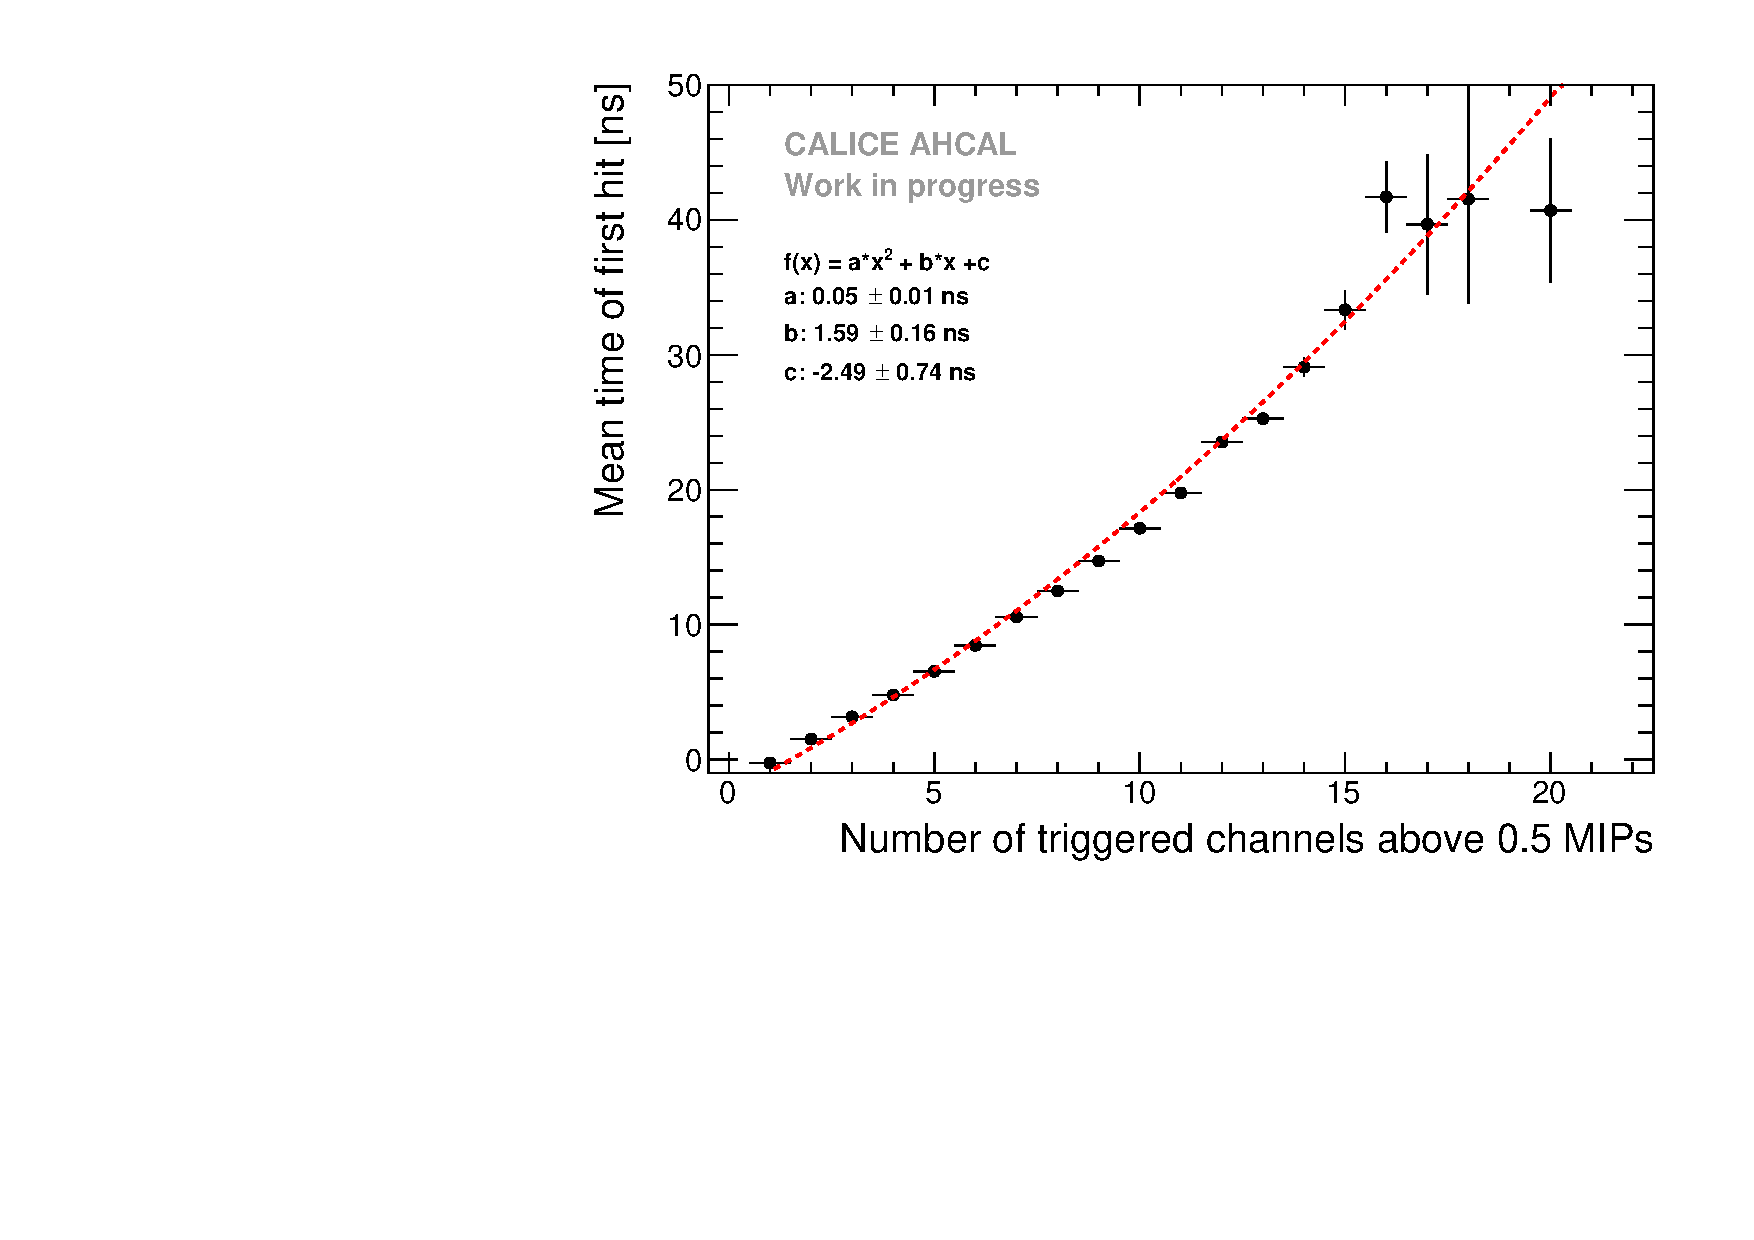
\includegraphics[width=1\textwidth]{../Thesis_Plots/Timing/Electrons/Plots/NumberHits_Dependance_AllEnergies.pdf}
		\caption{Time of the first hit as a function of the number of triggered channels above 0.5 MIP in a chip for all electron energies.}\label{fig:nhits_profile}
	\end{subfigure}
	\hfill
	\begin{subfigure}[t]{0.5\textwidth}
		\centering
		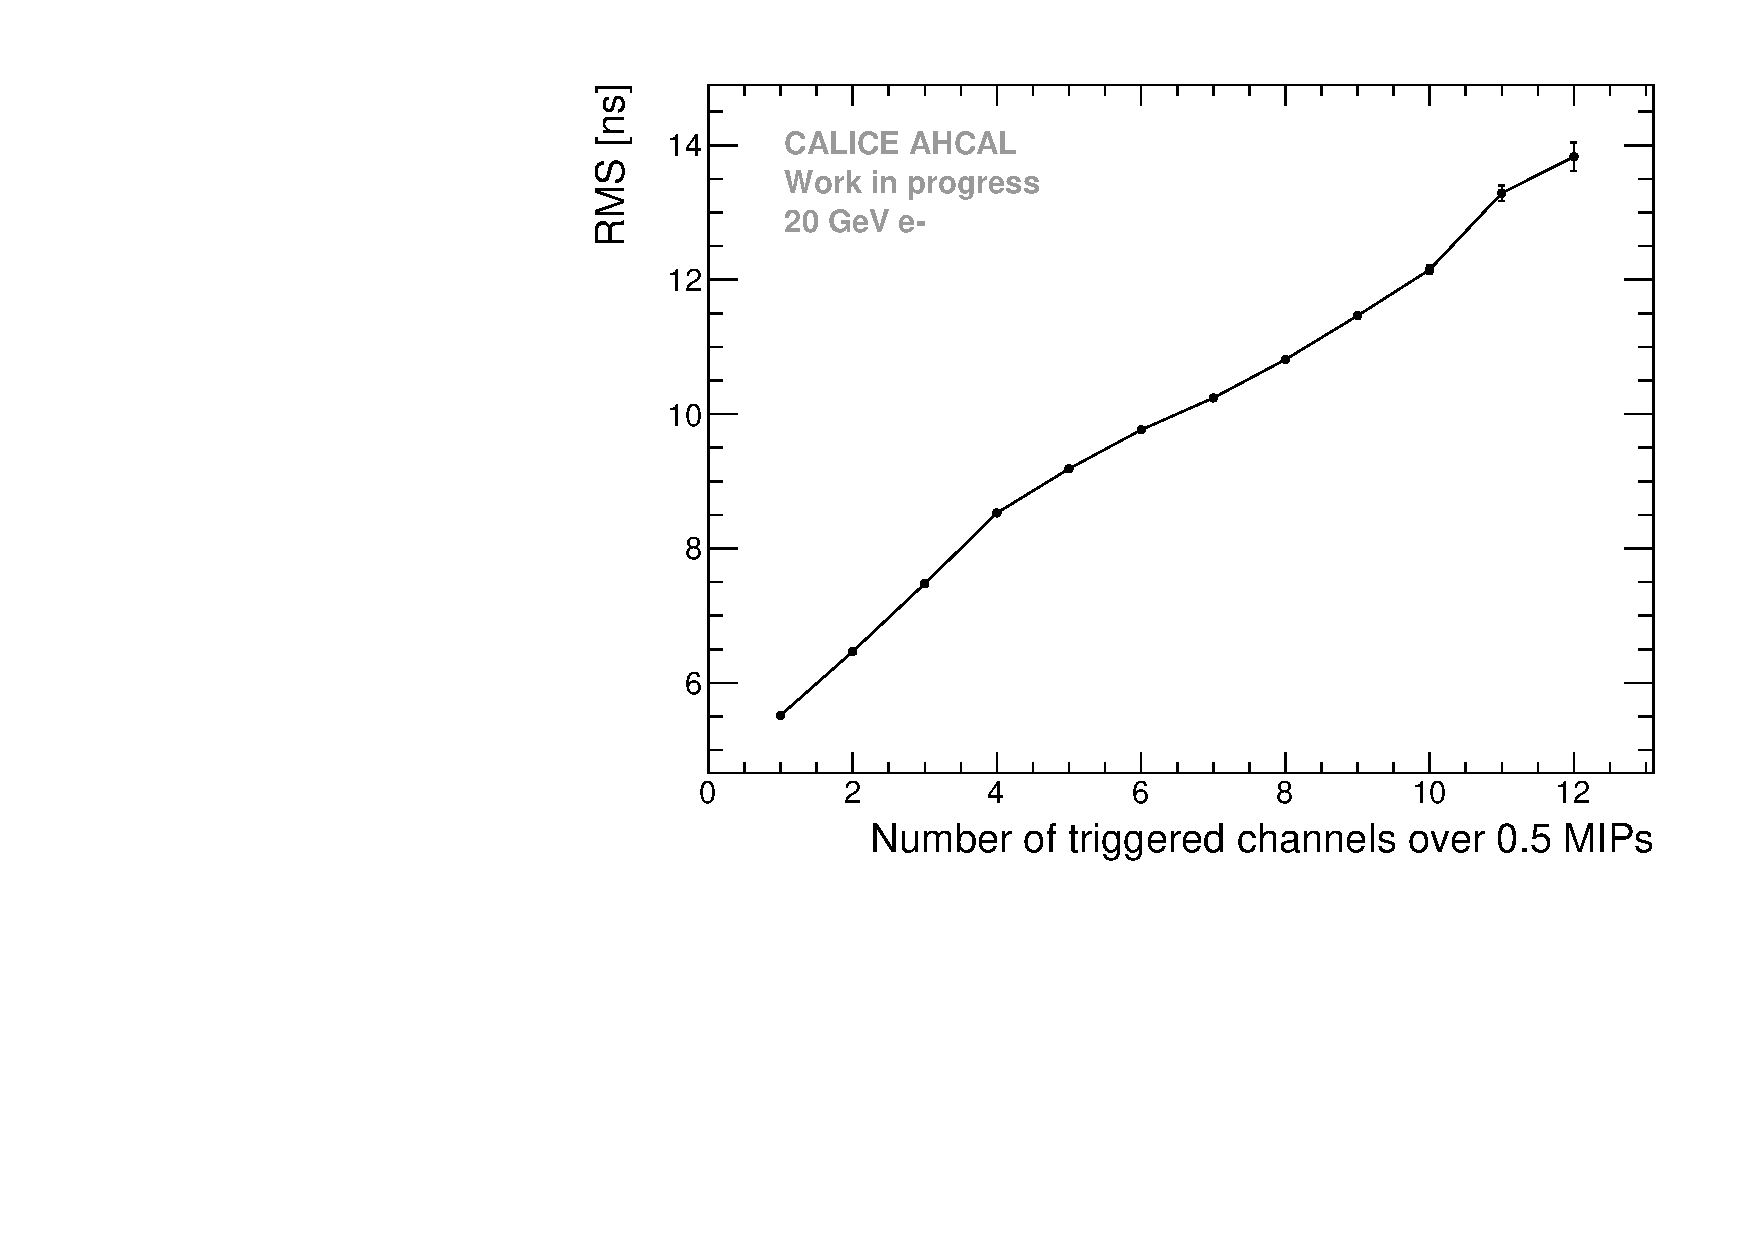
\includegraphics[width=1\textwidth]{../Thesis_Plots/Timing/Electrons/Plots/ParametrisationPedestalShift_20GeV.pdf}
		\caption{RMS of the time of first hit function of the number of triggered channels above 0.5 MIP for 20 GeV electrons.}\label{fig:RMS_nHits}
	\end{subfigure}
	\caption{\subref{fig:nhits_profile}) Mean time of the hit as function of the number of triggered channels above 0.5 MIP in a chip. The mean time shift upwards with the increase of triggers leading to large tails in the time distribution. The plot is obtained by combining all electron energies and a polynomial fit is done. \subref{fig:RMS_nHits}) The RMS of the time distribution can increase up to 10-15 ns for a high number of triggered channels.}
\end{figure}

\section{Time of the first hit for electrons}
\label{subsec:Electron_Final}

The distribution of the time of the first for 20 GeV is shown in figure \ref{fig:timing_electrons_corr} after correction as function of the triggered channels. The correction improves the RMS of the distribution by around 12.1\%, as well as the distribution appears more gaussian-like. However, there is still a discrepancy (around 33.7\%) with the time resolution obtained for muons (5.2 ns). This is due to the fact that not only the mean time shifts but that the RMS also increases as a function of the number of hits as seen in figure \ref{fig:RMS_nHits} and can't be corrected (each individual distributions have been checked). In order for the simulation to match the data, the increase of the width of the time distribution has to be parametrized from the data. More details can be read in the appendix \ref{appendix:ped_shift}.

\begin{figure}[htbp!]
	\begin{subfigure}[t]{0.5\textwidth}
		\centering
		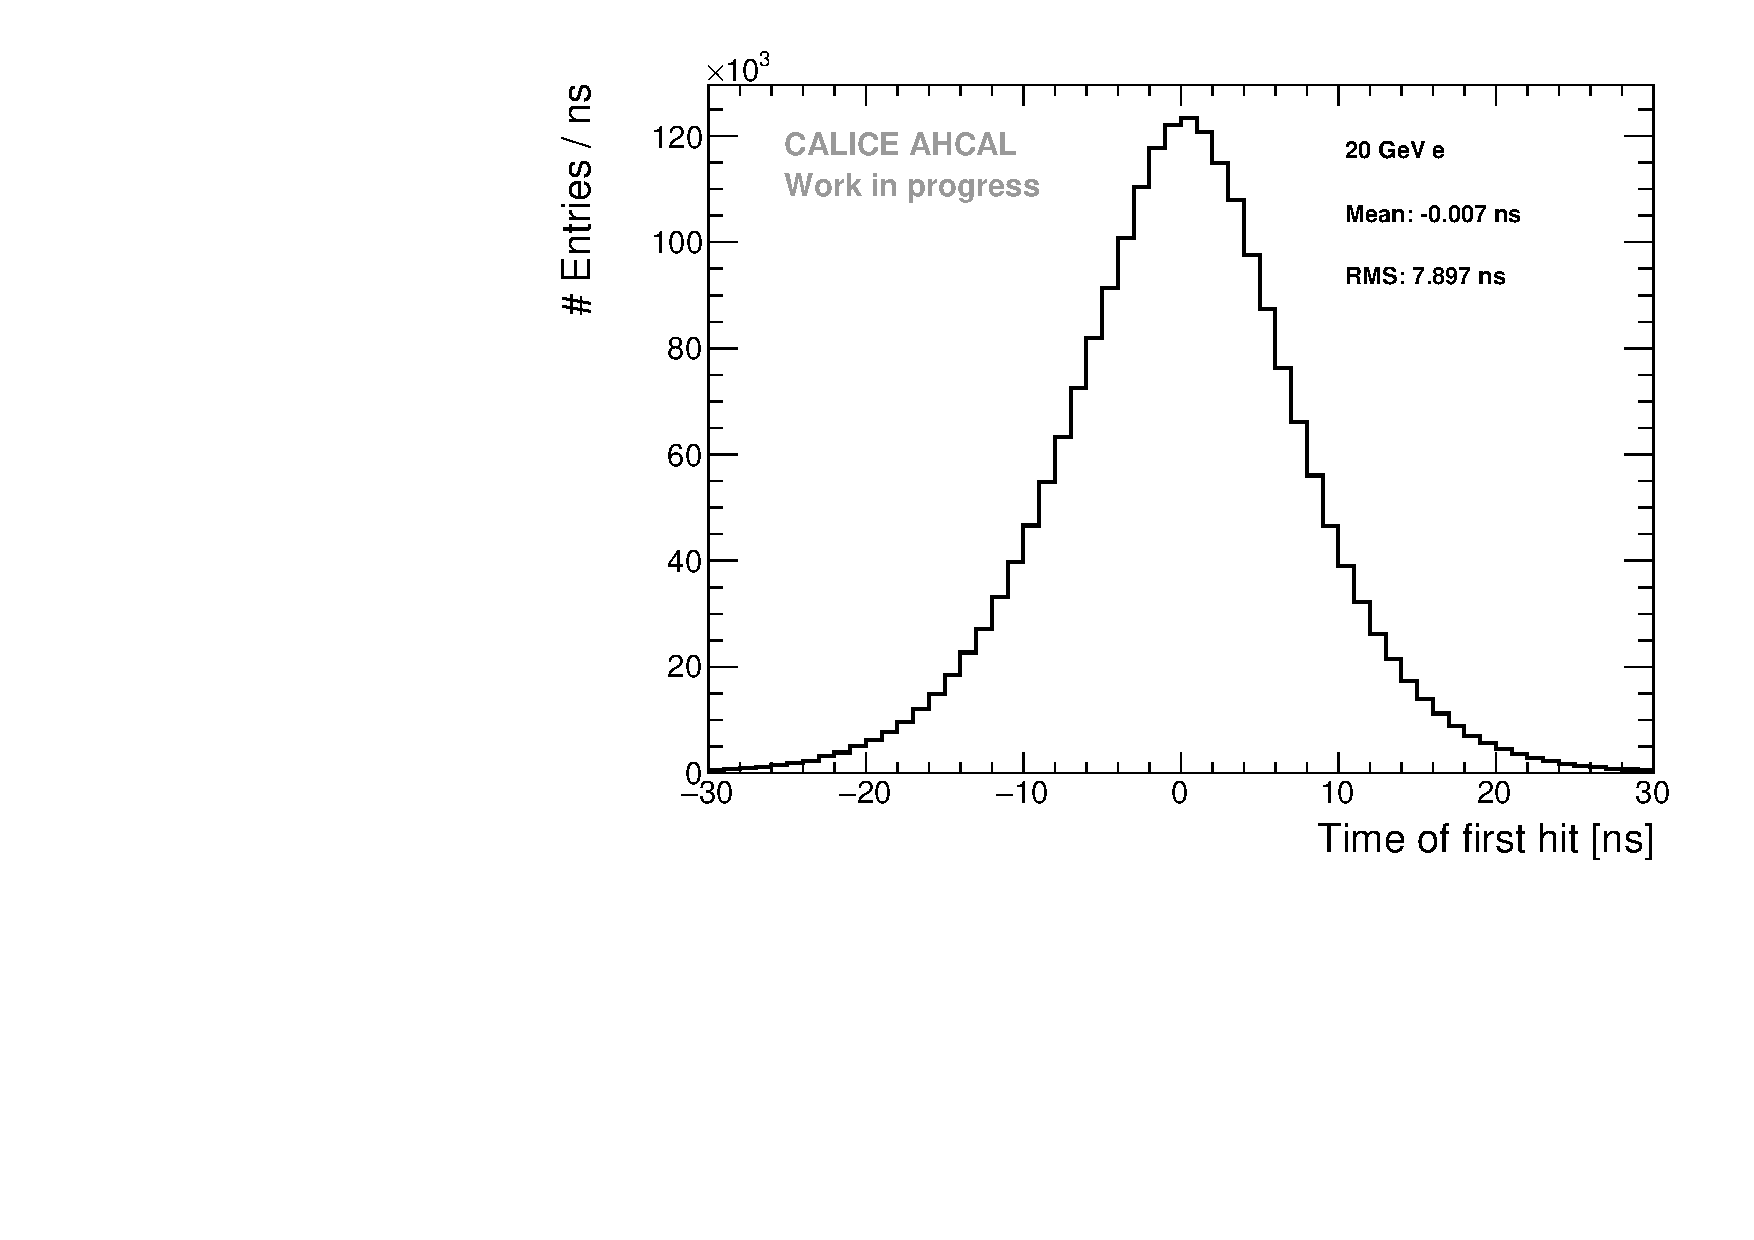
\includegraphics[width=1\textwidth]{../Thesis_Plots/Timing/Electrons/Plots/Timing_AllLayers_20GeV.pdf}
		\caption{}\label{fig:timing_electrons_corr}
	\end{subfigure}
	\hfill
	\begin{subfigure}[t]{0.5\textwidth}
		\centering
		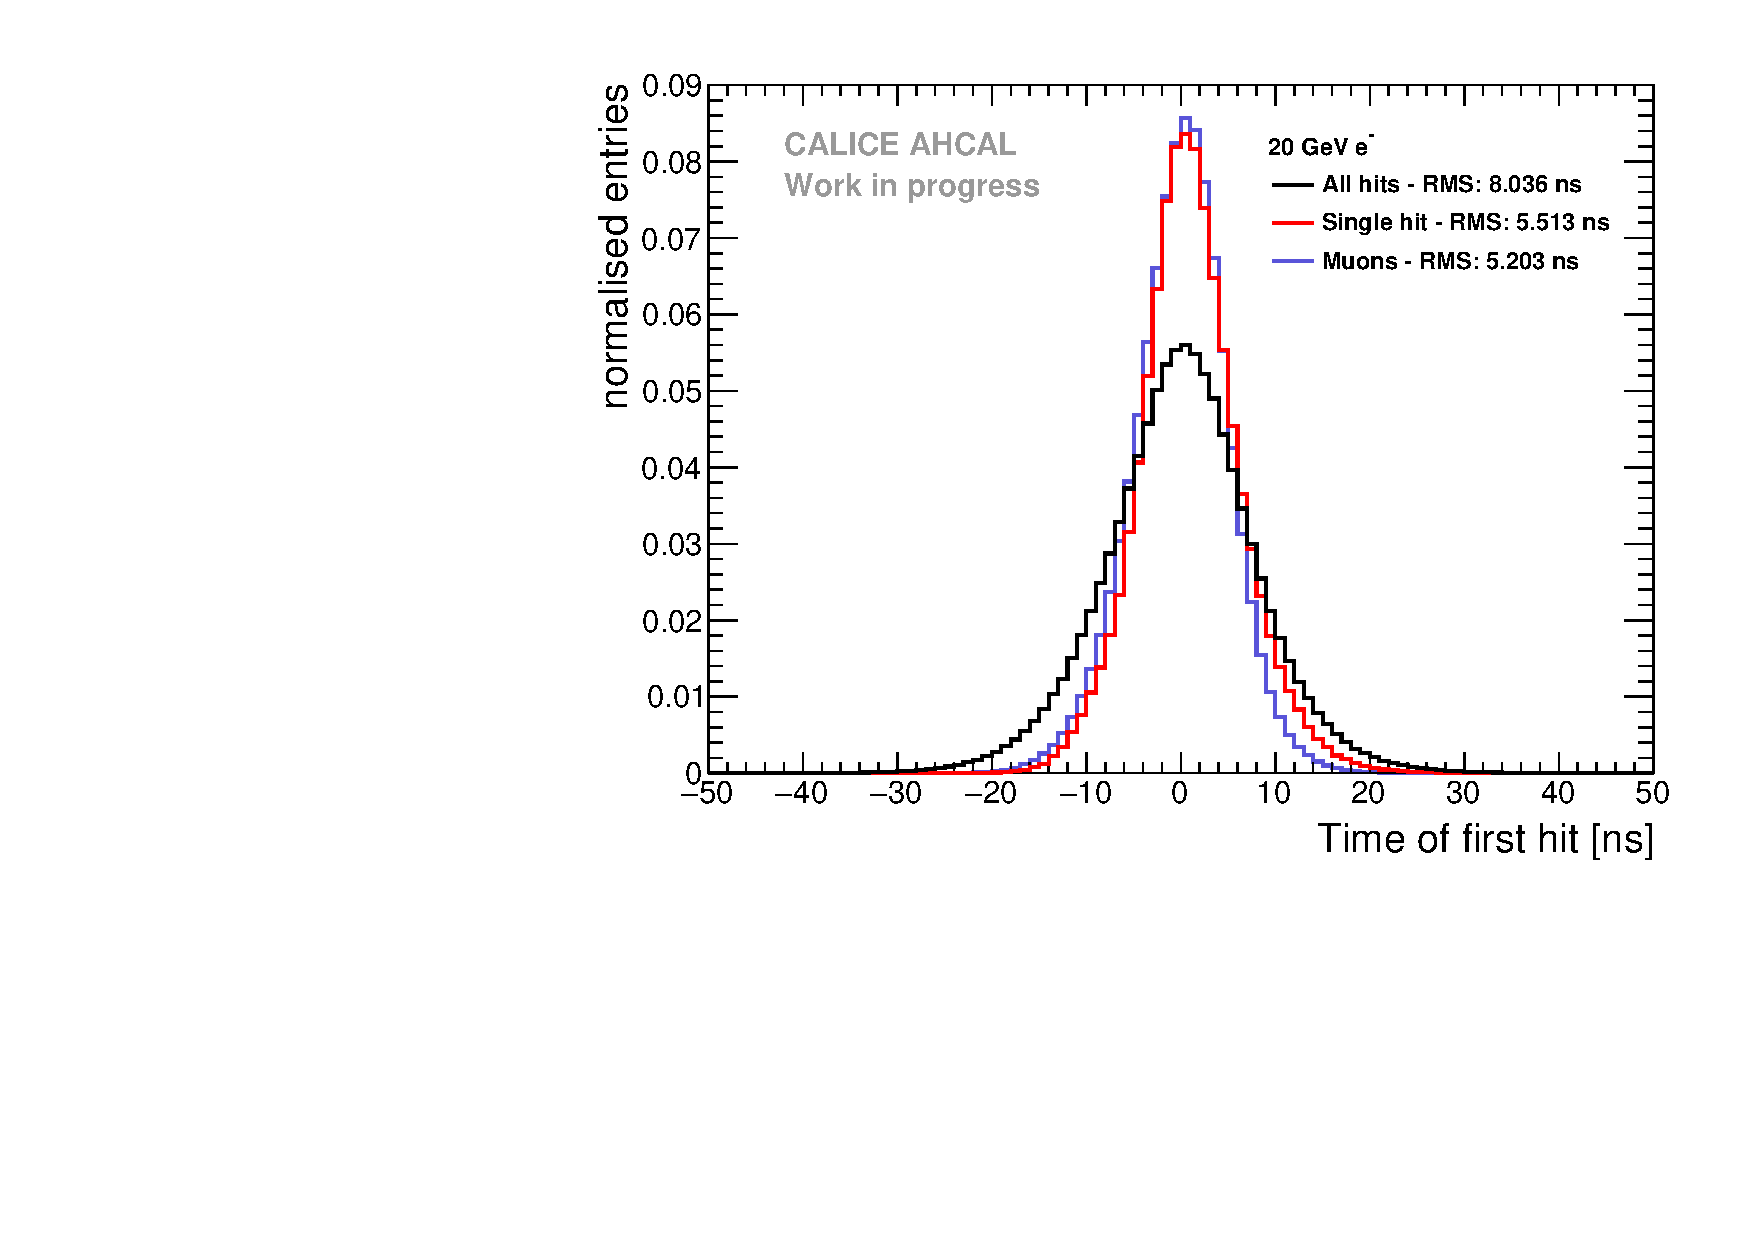
\includegraphics[width=1\textwidth]{../Thesis_Plots/Timing/Electrons/Plots/ComparisonAll_ElectronsSingleHit.pdf}
		\caption{}\label{fig:timing_electron_muon_comp}
	\end{subfigure}
	\caption{\subref{fig:timing_electrons_corr}) Time of the first hit distribution for 20 GeV electrons after number of triggered channel correction, $\mu$ = -0.018 ns, RMS = 7.84 ns. \subref{fig:timing_electron_muon_comp}) Comparison of the electron data sample, the time distribution is very similar to the muon one if only events with single hits in a chip are taken.}
\end{figure}

A comparison with the muon data has been done in order to cross-check the calibration as well as the correction as seen in figure \ref{fig:timing_electron_muon_comp}. If only single hits in a chip are taken, the time resolution obtained is very similar to the time resolution observed in muons (around 5.2\% difference). All electron runs have been checked to validate the correction and calibration procedure. The figure \ref{fig:all_electron_energies} shows the comparison from 10 GeV to 50 GeV. The distributions are in agreement for all energies. The RMS varies between 7.86 ns at 10 GeV to 8.5 ns at 50 GeV corresponding to an increase of the resolution of about 8\%.

\begin{figure}[htbp!]
	\centering
	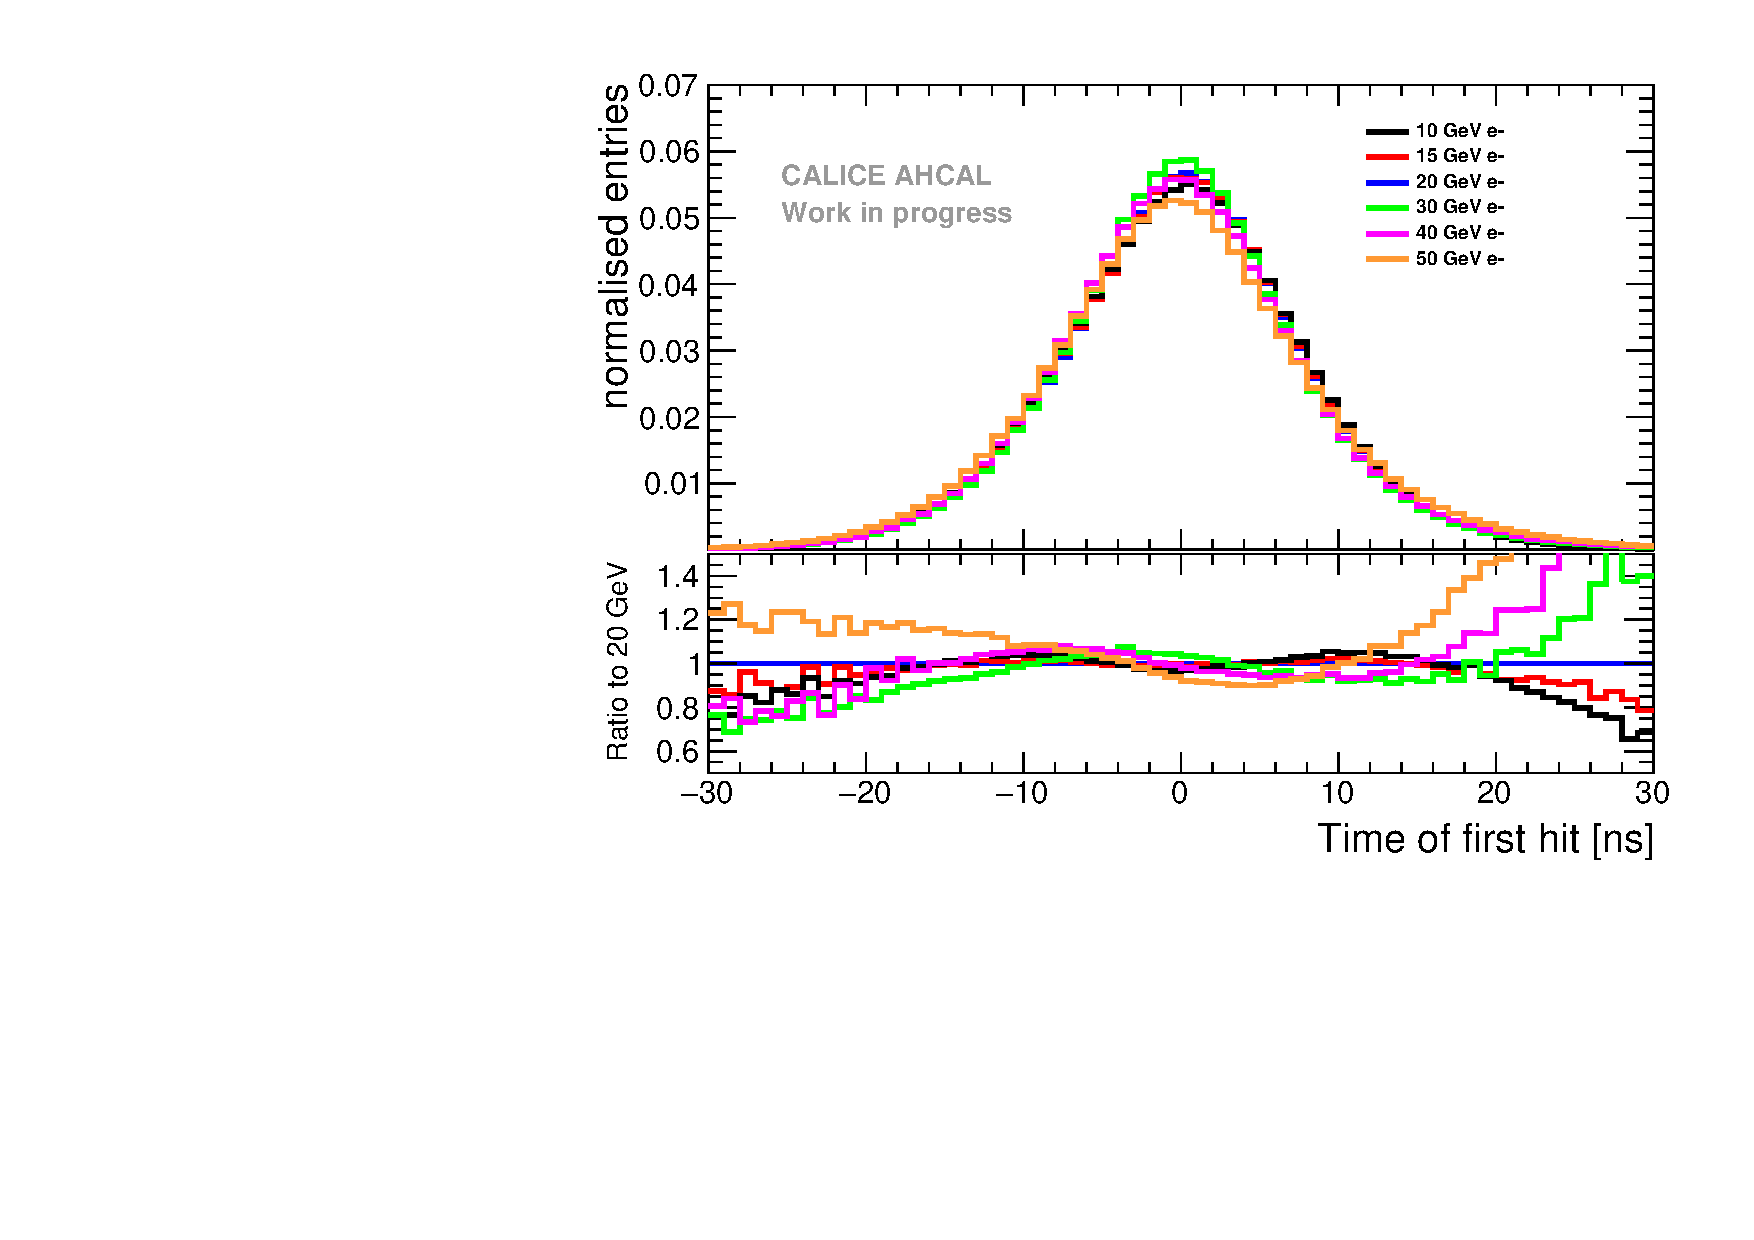
\includegraphics[width=0.6\textwidth]{../Thesis_Plots/Timing/Electrons/Plots/ComparisonDataEnergies.pdf}
	\caption{Comparison of the time of first hit distribution for all electron energies.}
	\label{fig:all_electron_energies}
\end{figure}

\section{Influence of the detector inhomogeneity}
\label{subsec:det_inhomo}

A study has been performed to estimate the influence of the detector inhomogeneity in space on timing. For this, only events in which the centre of gravity in x and y is within the 4 centre tiles of the detector are selected. This has been performed for 10 and 50 GeV electron beam energy. The difference between the distribution helps to estimate the systematic uncertainty due to the inhomogeneity of the detector to which electrons are very sensitive to.

\begin{figure}[htbp!]
	\begin{subfigure}[t]{0.5\textwidth}
		\centering
		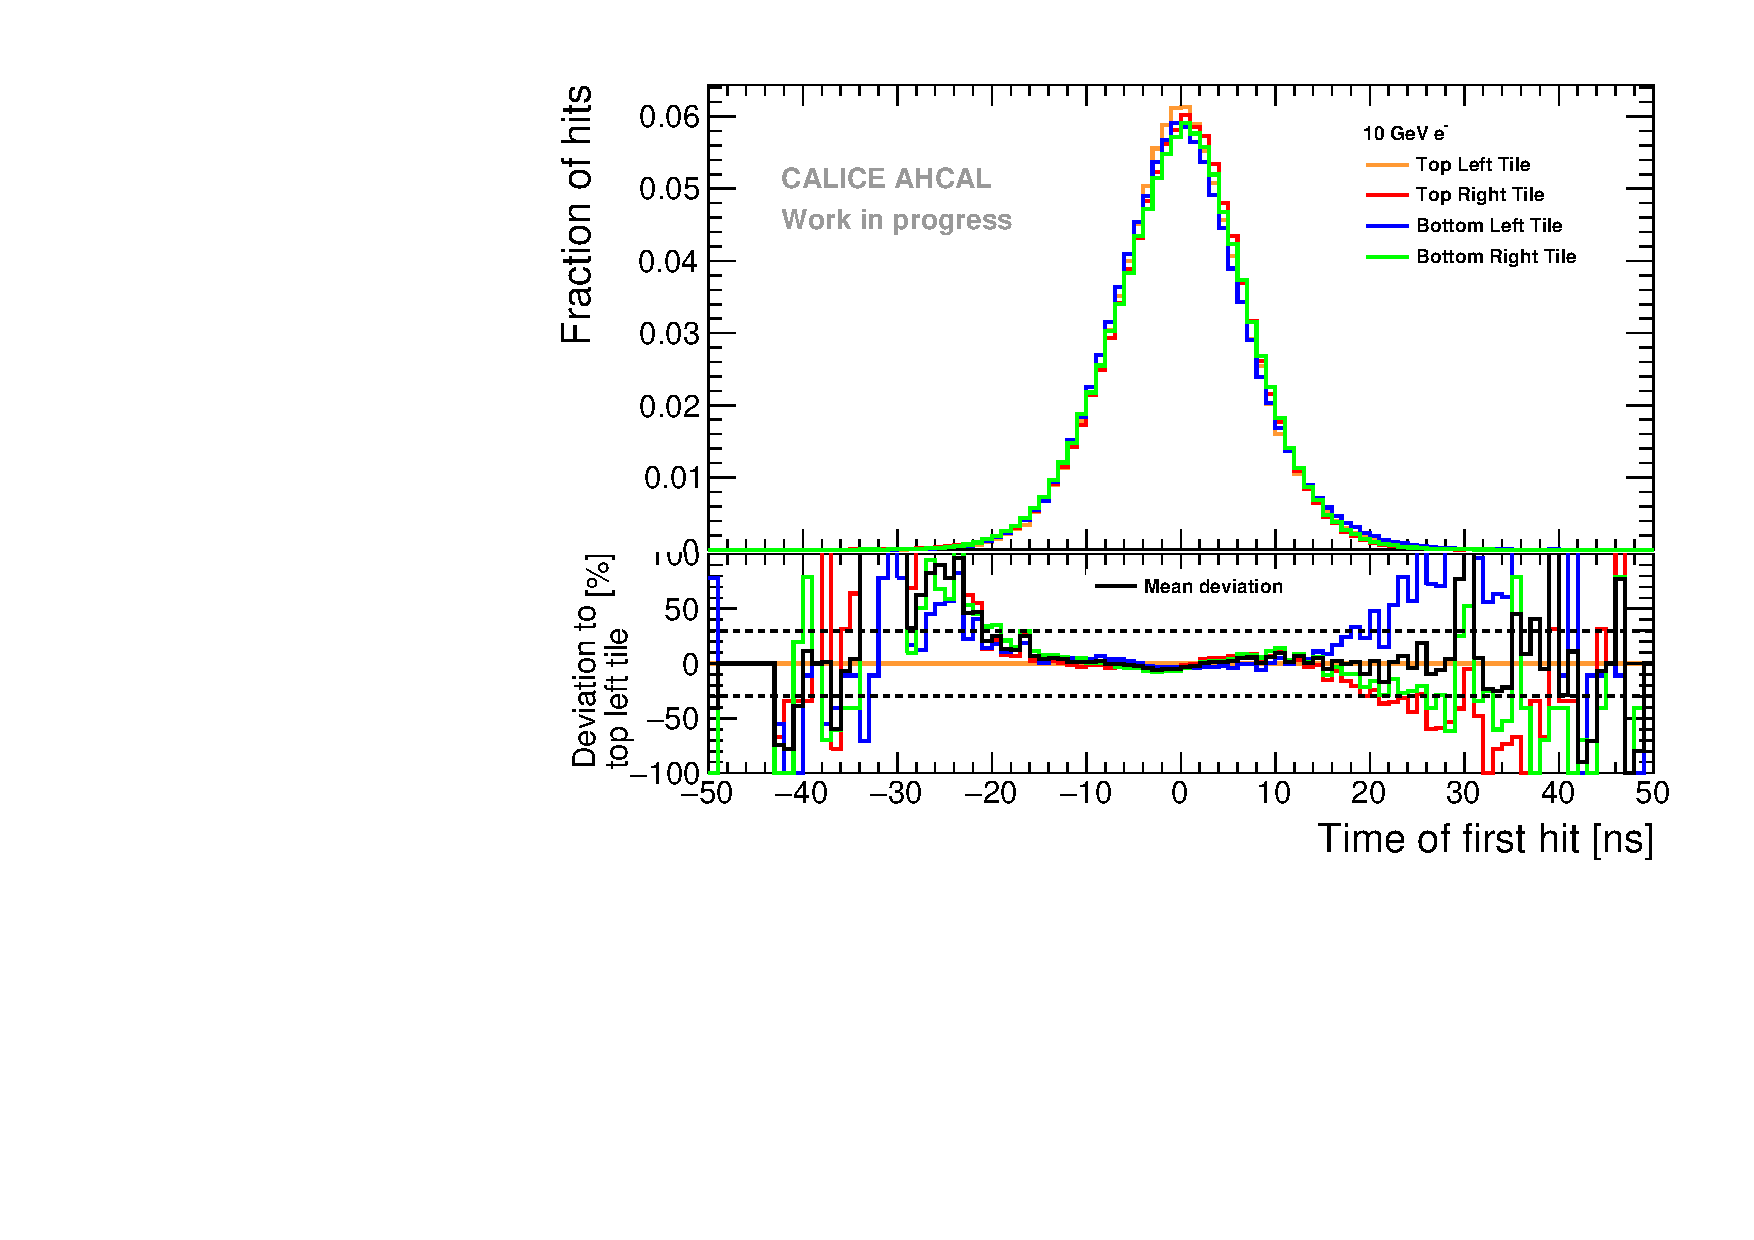
\includegraphics[width=1\textwidth]{../Thesis_Plots/Timing/Electrons/Plots/Systematic_Inhomogeneity_10GeV.pdf}
		\caption{}\label{fig:timing_inhomo_10GeV}
	\end{subfigure}
	\hfill
	\begin{subfigure}[t]{0.5\textwidth}
		\centering
		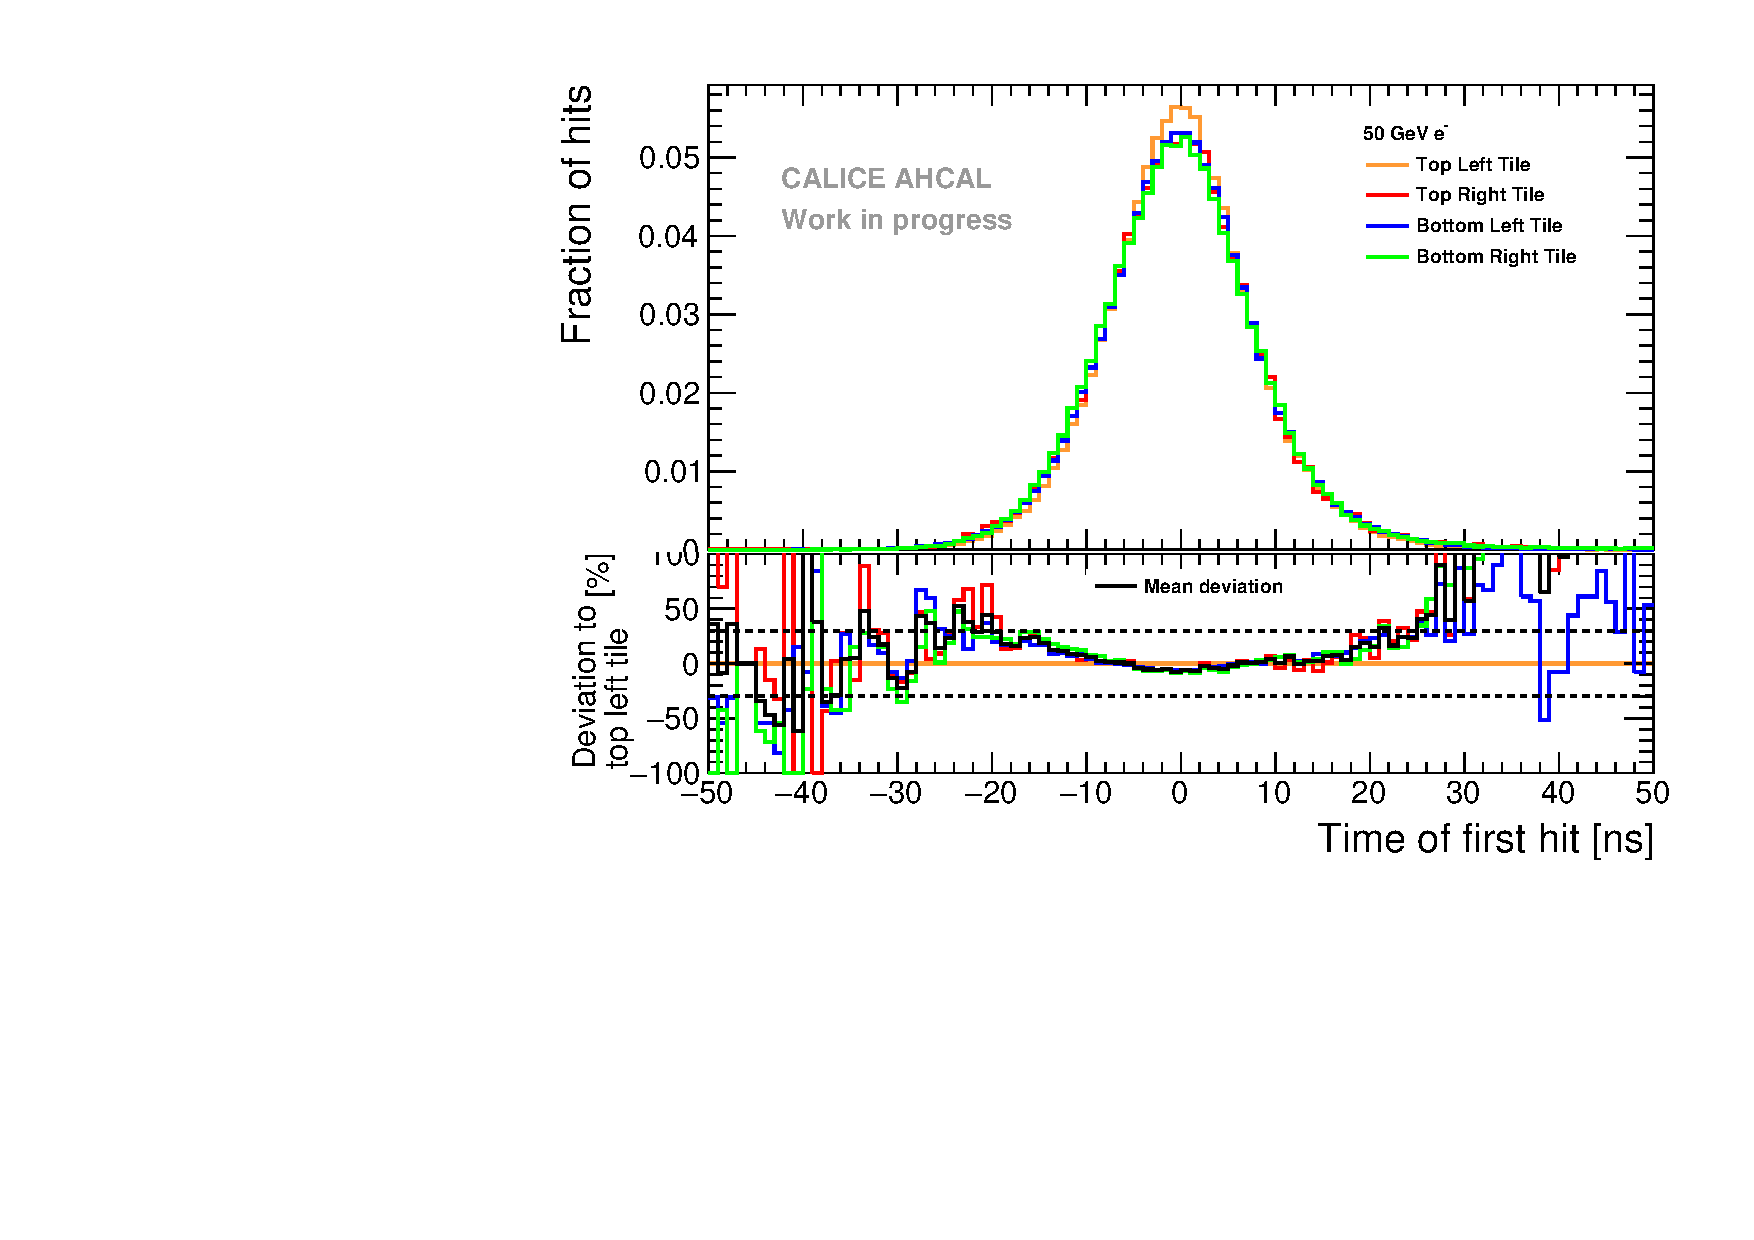
\includegraphics[width=1\textwidth]{../Thesis_Plots/Timing/Electrons/Plots/Systematic_Inhomogeneity_50GeV.pdf}
		\caption{}\label{fig:timing_inhomo_50GeV}
	\end{subfigure}
	\caption{\subref{fig:timing_inhomo_10GeV}) Time of the first hit distribution for all four middle tiles with 10 GeV electron beam. \subref{fig:timing_inhomo_50GeV}) Time of the first hit distribution for all four middle tiles with 50 GeV electron beam. All distribution are within 10-20\% in the core.}
\end{figure}

The figures \ref{fig:timing_inhomo_10GeV} and \ref{fig:timing_inhomo_50GeV} show the time distribution for each tile at 10 and 50 GeV respectively. The ratio shown is compared to the top left centre tile. One can see that for both energies, the distributions are within a 10-20\% agreement with the region [-20, 20] ns. Therefore a conservative systematic uncertainty of 20\% is assigned to electron and pion data in the following. % Need to add argument why -20, 20 ns... maybe do -50, 200?%

\section{Portability of the calibration}

A check on the validity of the calibration for other data-taking periods has been performed on another dataset from a testbeam at DESY II in May 2016. The goal was to reuse the calibration constants obtained and apply them to another dataset in order to understand how transportable is the time calibration. The setup was composed of the same four big layers used at CERN in July 2015. In order to have enough hits in all layers, an aluminum absorber of 3 $X_{0}$ was placed in front of the detector in a 3 GeV electron beam.

\begin{figure}[htbp!]
	\centering
	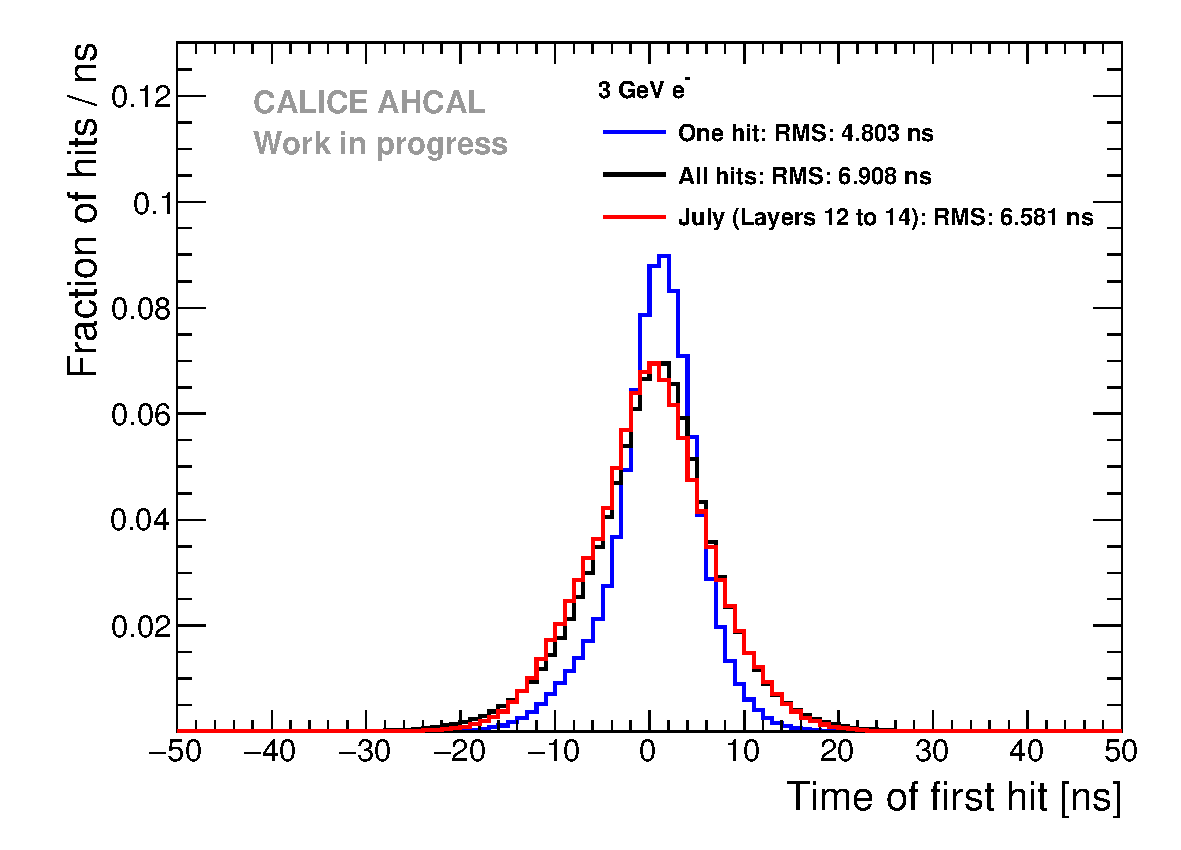
\includegraphics[width=0.7\textwidth]{../Thesis_Plots/Timing/Electrons/Plots/Timing_May2016_BigLayers.pdf}
	\caption{Time of the first hit distribution for 3 GeV electron showers at the DESY II testbeam in May 2016 combining layer 13 and 14.}\label{fig:TBMay2016}
\end{figure}

The same calibration constants were used except a re-calibration of the trigger channels ($T_{0}$) was performed. This was to be done due to a different cabling and trigger logic. The figure \ref{fig:TBMay2016} shows the distribution of the time of first hits for layer 13 and 14. The time resolution obtained of 7 ns is slighly better than the time resolution obtained in July 2015. The difference may come from the fact a different configuration was used in the testbeam at CERN compared to DESY but also the lower beam energy. We can learn from this study, that the time calibration constants determined in a specific dataset can also be used for another dataset with the same layers.

\section{Systematic uncertainties}

For a significant assesment of differences observed between data and simulations, systematic uncertainties must be evaluated. Several possible sources were identified:

\begin{itemize}
	% \item MIP Energy Scale: An error on the MIP energy scale needs to be converted in time when looking at the dependence of time with hit energy. An error of 0.5\% is taken. Using simulation, this can be converted into time. For muon and electron beams, it has mostly no effects. For pion beams, it ranges from XXX ns at 0.5 MIP to XXX ns at 1 MIP.
	\item Non-Linearity correction: A non-linearity correction is applied to the data as explained in section \ref{subsec:lin_corr}. The residuals of the correction give a systematic error at the level of 0.2 ns.
	\item Time walk correction: In the same way as for the non-linearity correction, the error obtained from the residuals of the correction is in the order of 0.2 ns.
	\item Number of triggered channels correction: the correction for the number of triggered channels over 0.5 MIP in a chip results in a residual on the timing in the order of 1 ns. This systematic error is the most dominant over all other uncertainties.
	\item Smearing parametrization: A parametrization was obtained from data for the width of the time smearing as function of the number of triggered channels. An error band was obtained by comparing all electron energies as explained in appendix \ref{appendix:ped_shift}. This is applied to simulation for systematics.
	\item Determination of the offset to $t=0$: A shift of the time distribution at zero is done for each layer. The uncertainty of this shift varies between 0.05 to 0.1 ns for data. In this case, a conservative uncertainty of 0.1 ns is used. For simulation, the shift can be calculated easily using a simple time of flight correction $T_{of} = \frac{z_{layer}}{c}$ with $c$ the speed of light and $z_{layer}$ the z position of a layer. For this a uncertainty of 3 mm is taken in z corresponding to 0.01 ns uncertainty in timing.
	\item Position relative of the detector to the beam: The detector was positioned in a way that the beam hits mostly the centered tiles. The uncertainty of the position of the layers is at the millimeter level. Thus a conservative uncertainty of a tile (3 cm) is taken. This uncertainty converted to time using QGSP\_BERT\_HP varies between 0.36 ns at $r = 1.5$ cm to 1.27 ns at $r = 19.5$ cm for the small layers and between 0.15 ns at $r = 1.5$ cm to 0.67 ns at $r = 31.5$ cm for the big layers using 10 GeV data.
	\item Cross-talk: No measurement for optical cross-talk between tiles is available and from previous measurements it varies between 10\% and 18\%. These are used for systematics in simulation only for the layers 4 to 10.
	\item Detector inhomogeneities: As explained in section \ref{subsec:det_inhomo}, variations in the absolute number of entries in each time bins can be observed. The variations are between 10-20\% thus a conservative error of 20\% is used for the time distribution.
	\item Absolute number of events: In the pion data, some possible contamination from multi-particle events may be present still after the selection. Thus the number of absolute pion events is not known. A conservative error of 10\% when comparing data to simulation for the absolute number of hits per time bin.
\end{itemize}

The systematic uncertainties are added in quadrature for the full systematic uncertainty. For comparison between data-MC of the number of hits per time bin, an uncertainty of 20\% for muons/electrons and 30\% for pions is used. For the distribution of time versus energy, the systematic uncertainty is resulting at 1.04 ns. For the distribution of time versus radius, the systematic uncertainty is varying between 0.36 ns at small radius to 1.54 ns at large radius for the small layers and from 0.15 ns at small radius to 0.95 ns at large radius for the big layers. The table \ref{table:time_syst} sums up the systematic uncertainties used in the analysis.
%% Systematics from number of hits may be underestimated... %
{
\renewcommand{\arraystretch}{1.2}
\begin{table}[htb!]
	\centering
	\caption{Summary of systematic uncertainties.}
	\label{table:time_syst}
	\begin{tabular}{@{} |l|c| @{}}
		\hline
		\multicolumn{1}{|c|}{Uncertainty source} & Full uncertainty steel \\
		\hline
		% MIP Energy Scale & XXX-XXX ns \\
		Non-linearity residuals & 0.2 ns \\
		Time-walk residuals & 0.2 ns \\
		Number of triggered channels over 0.5 MIP residuals & 1 ns \\
		Offset to $t=0$ & 0.1 ns (data) 0.01 ns (MC) \\
		Position relative to the beam & 0.36-1.54 ns (SSF) 0.15-0.95 ns (BL) \\
		Cross-talk & 10-18\% \\
		Detector inhomogeneities & 20\% \\
		Number of absolute events & 10\% (pions) \\
		\hline
		\hline
		\multicolumn{2}{|c|}{Systematics combined} \\
		\hline
		data-MC hits per time bin & 20\% (muons/electrons) - 30\% (pions) \\
		data-MC vs hit energy & 1.04 ns \\
		data-MC vs hit distance to CoG & 1.10-1.86 ns (SSF) 1.05-1.41 ns (BL) \\
		\hline
	\end{tabular}
\end{table}
}

\section{Validation of the simulation}

\begin{table}[htb!]
	\centering
	\caption{Timing resolution extracted with a double Gaussian fit from muon data used for simulation.}
	\label{table:time_res_sim}
	\begin{tabular}{@{} cccccc @{}}
		\hline
		$\alpha_{1}$ & $\mu_{1}$ [ns] & $\sigma_{1}$ [ns] & $\alpha_{2}$ & $\mu_{2}$ [ns] & $\sigma_{2}$ [ns] \\
		\hline
		0.607352 & -0.699093 & 5.85891 & 0.391041 & 0.945272 & 3.4012 \\
		\hline
	\end{tabular}
\end{table}

The next step is to compare data with simulation. The timing resolution is extracted from muon data runs by fitting a double Gaussian to the data in the range [-50 ns, 50 ns] and is used to smear the timing of simulated calorimeter hits. The table \ref{table:time_res_sim} sums up the parameters used. The comparison for muons is shown in figure \ref{fig:sim_data_muon}. The comparison shows that in the full range, the difference between data and simulation is around 10-20\% maximum.

\begin{figure}[htbp!]
	\centering
	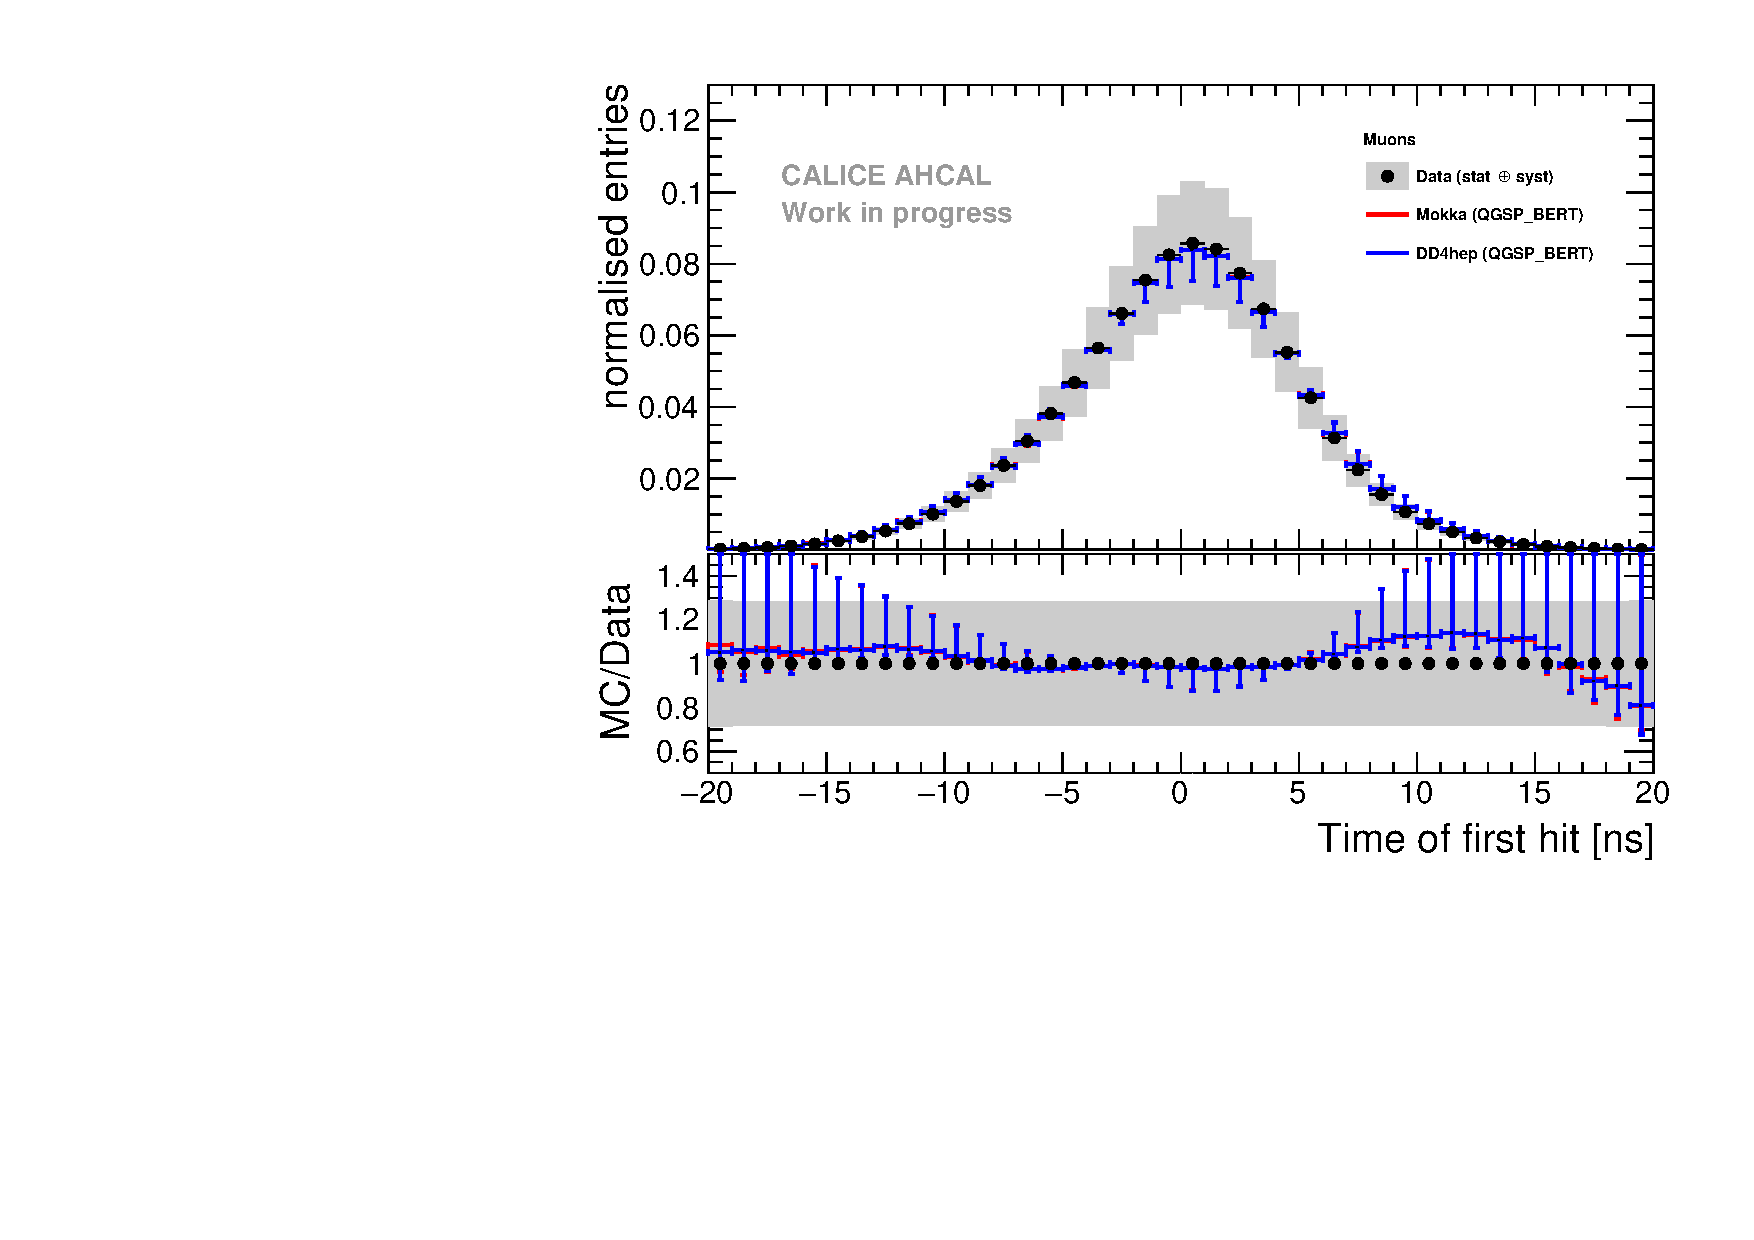
\includegraphics[width=0.6\textwidth]{../Thesis_Plots/Timing/Muons/Plots/Comparison_MokkaDD4hepData_Muons.pdf}
	\caption{Time of first hit for data and simulation between -20 and 20 ns.}
	\label{fig:sim_data_muon}
\end{figure}

In the next step, a comparison with electron data is necessary to validate the simulation. In addition to the muon resolution, a parametrization of the increase of the width of the time distribution as a function of the number of hits above 0.5 MIPs is added in simulation as described in appendix \ref{appendix:ped_shift}. Figure \ref{fig:sim_data_elec} shows this comparison.

\begin{figure}[htbp!]
	\begin{subfigure}[t]{0.5\textwidth}
		\centering
		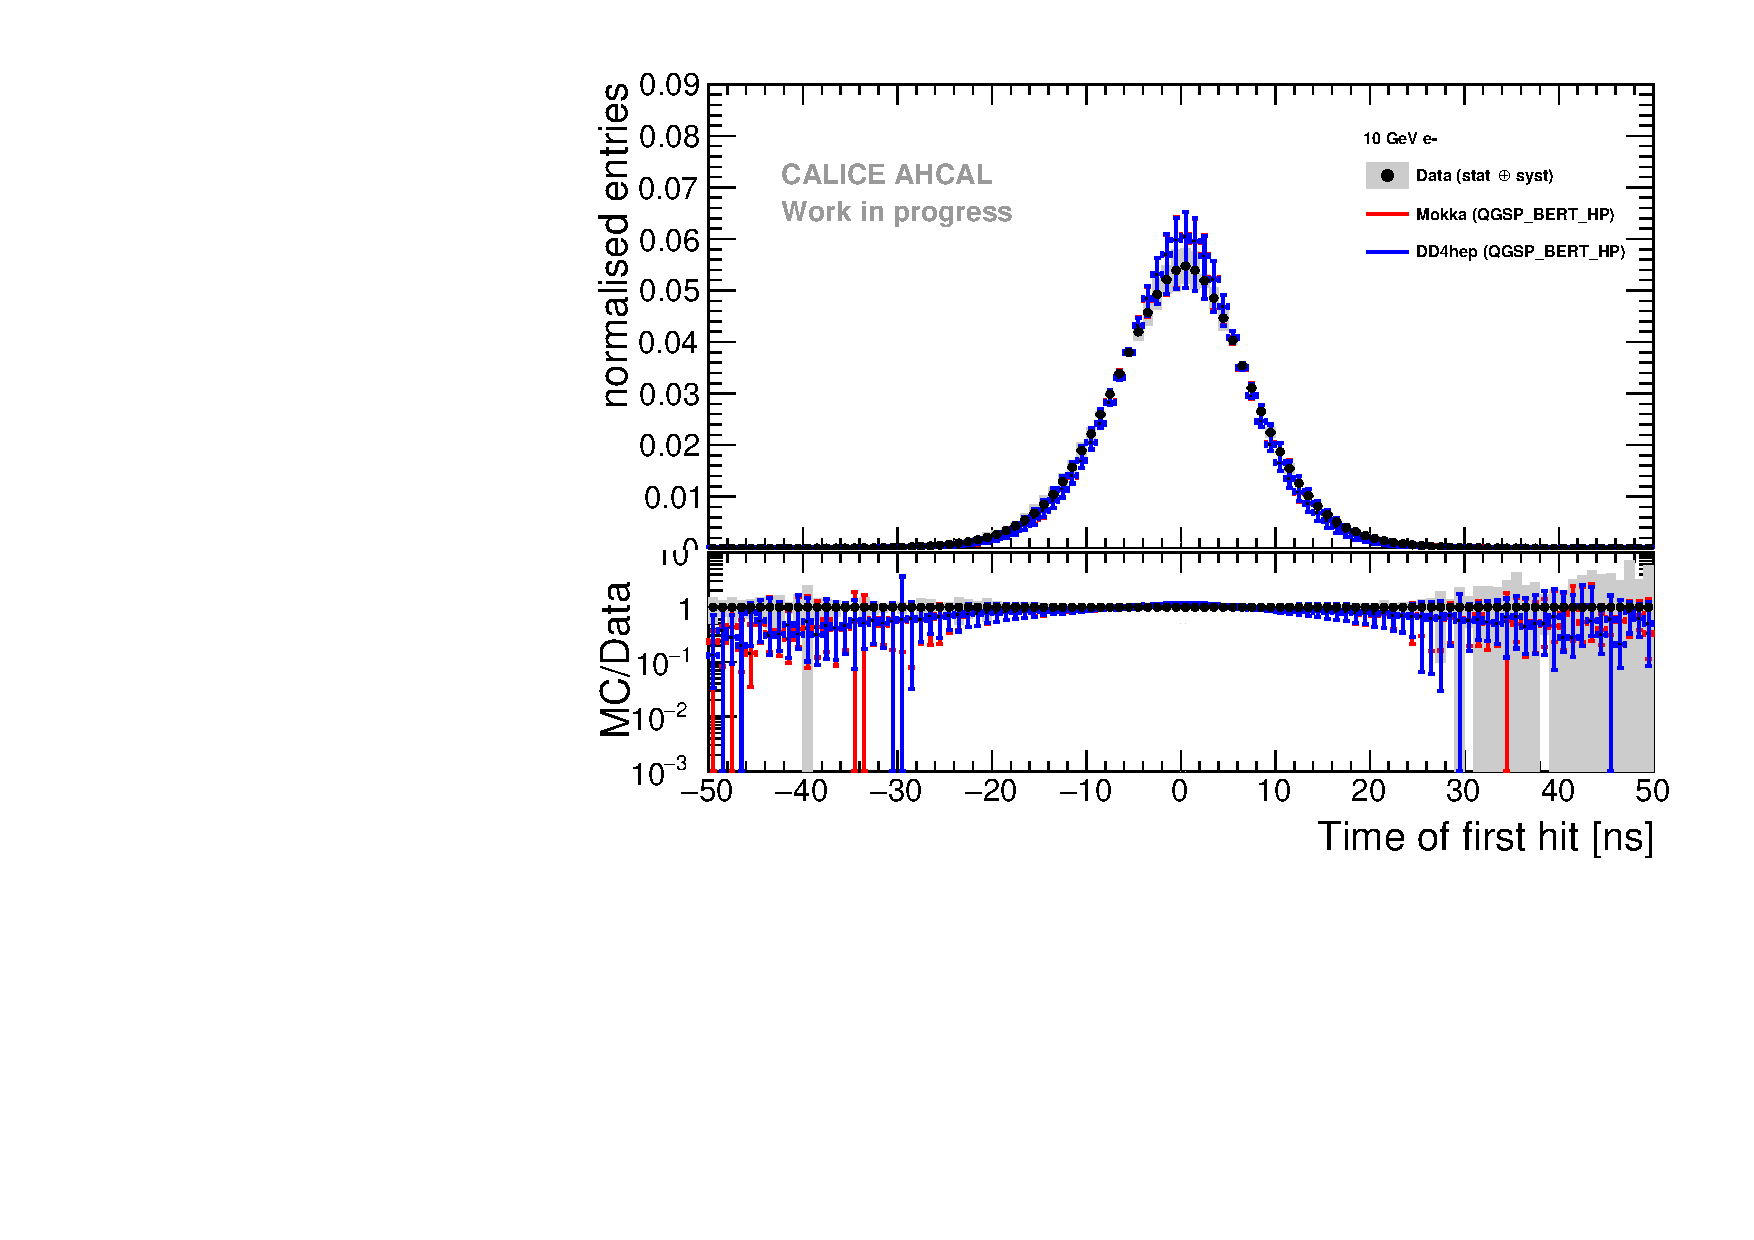
\includegraphics[width=1\textwidth]{../Thesis_Plots/Timing/Electrons/Plots/Comparison_SimData_Electrons10GeV.pdf}
		\caption{10 GeV.}\label{fig:elec_sim_data_10GeV}
	\end{subfigure}
	\hfill
	\begin{subfigure}[t]{0.5\textwidth}
		\centering
		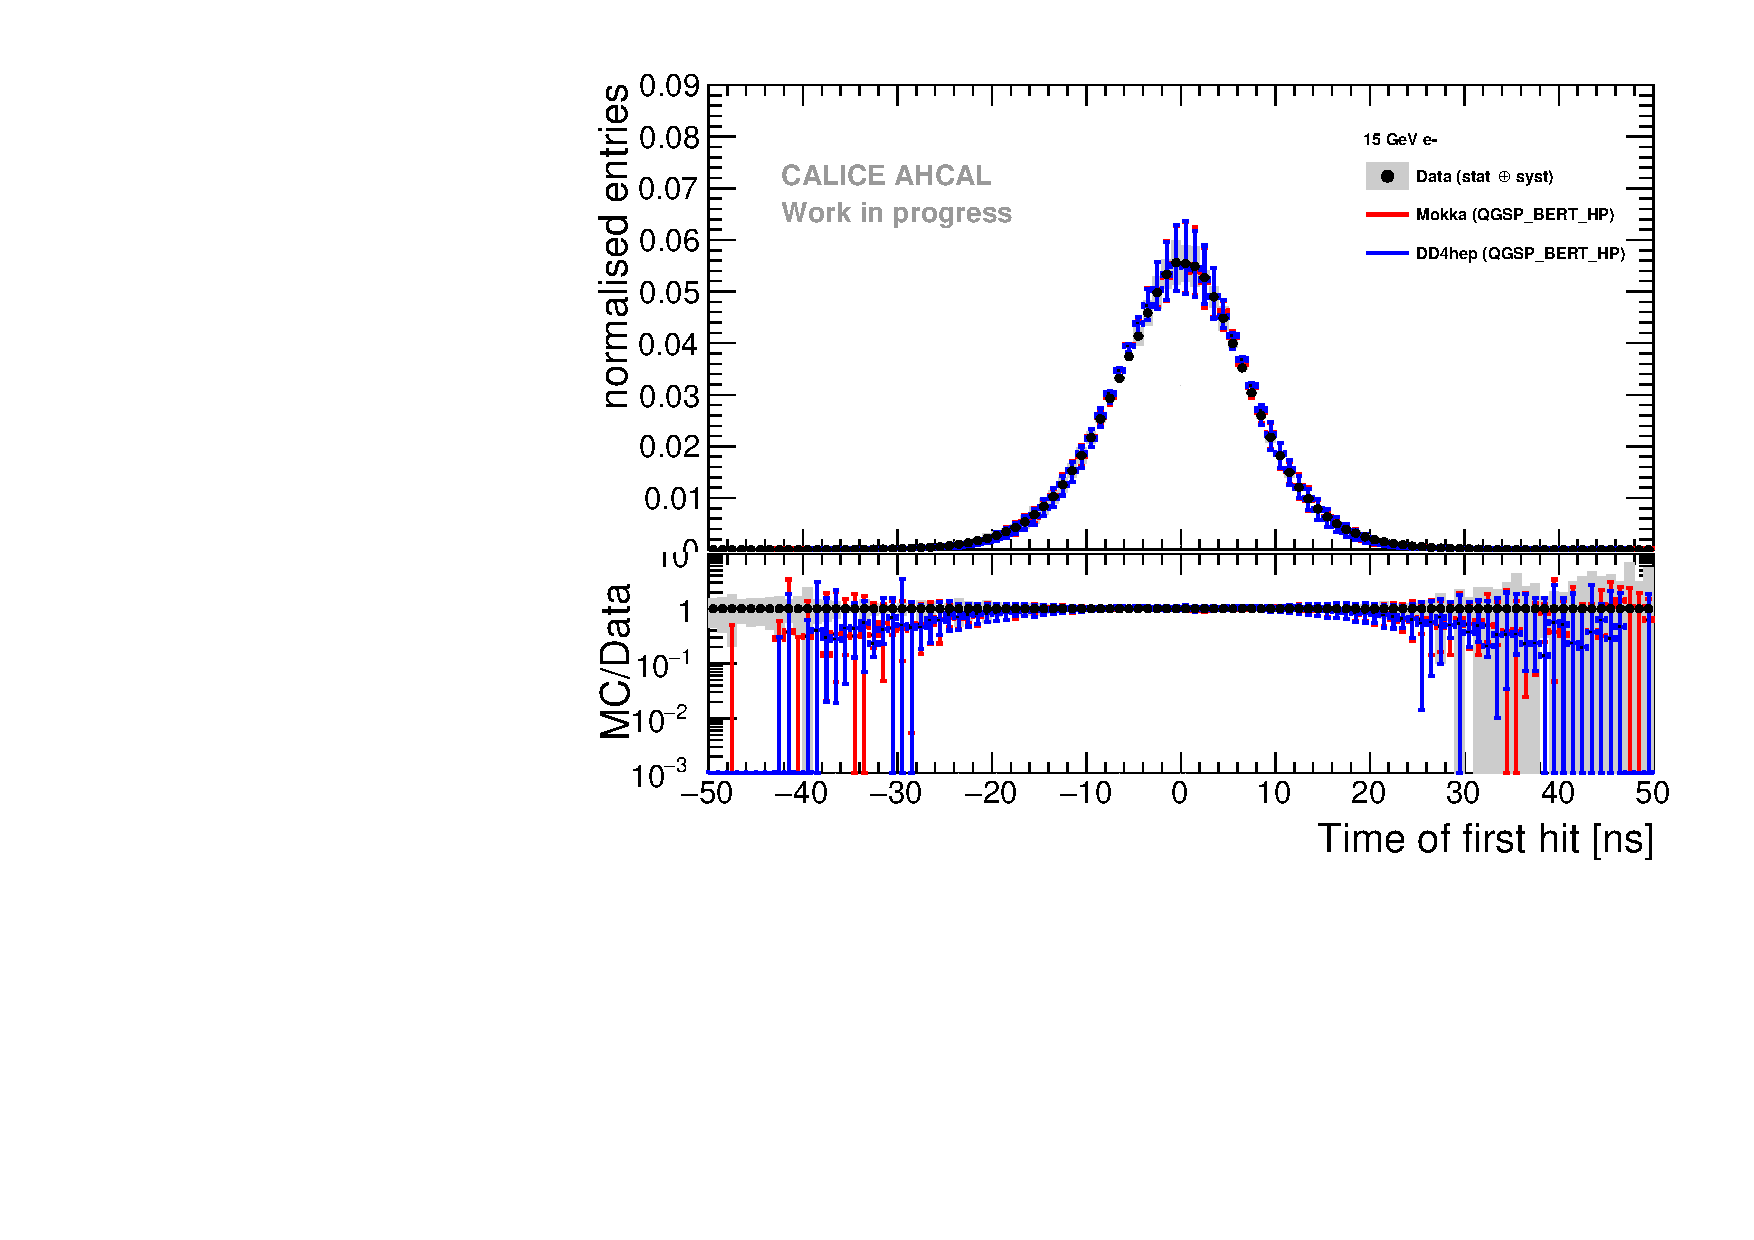
\includegraphics[width=1\textwidth]{../Thesis_Plots/Timing/Electrons/Plots/Comparison_SimData_Electrons15GeV.pdf}
		\caption{15 GeV.}\label{fig:elec_sim_data_15GeV}
	\end{subfigure}
	\hfill
	\begin{subfigure}[t]{0.5\textwidth}
		\centering
		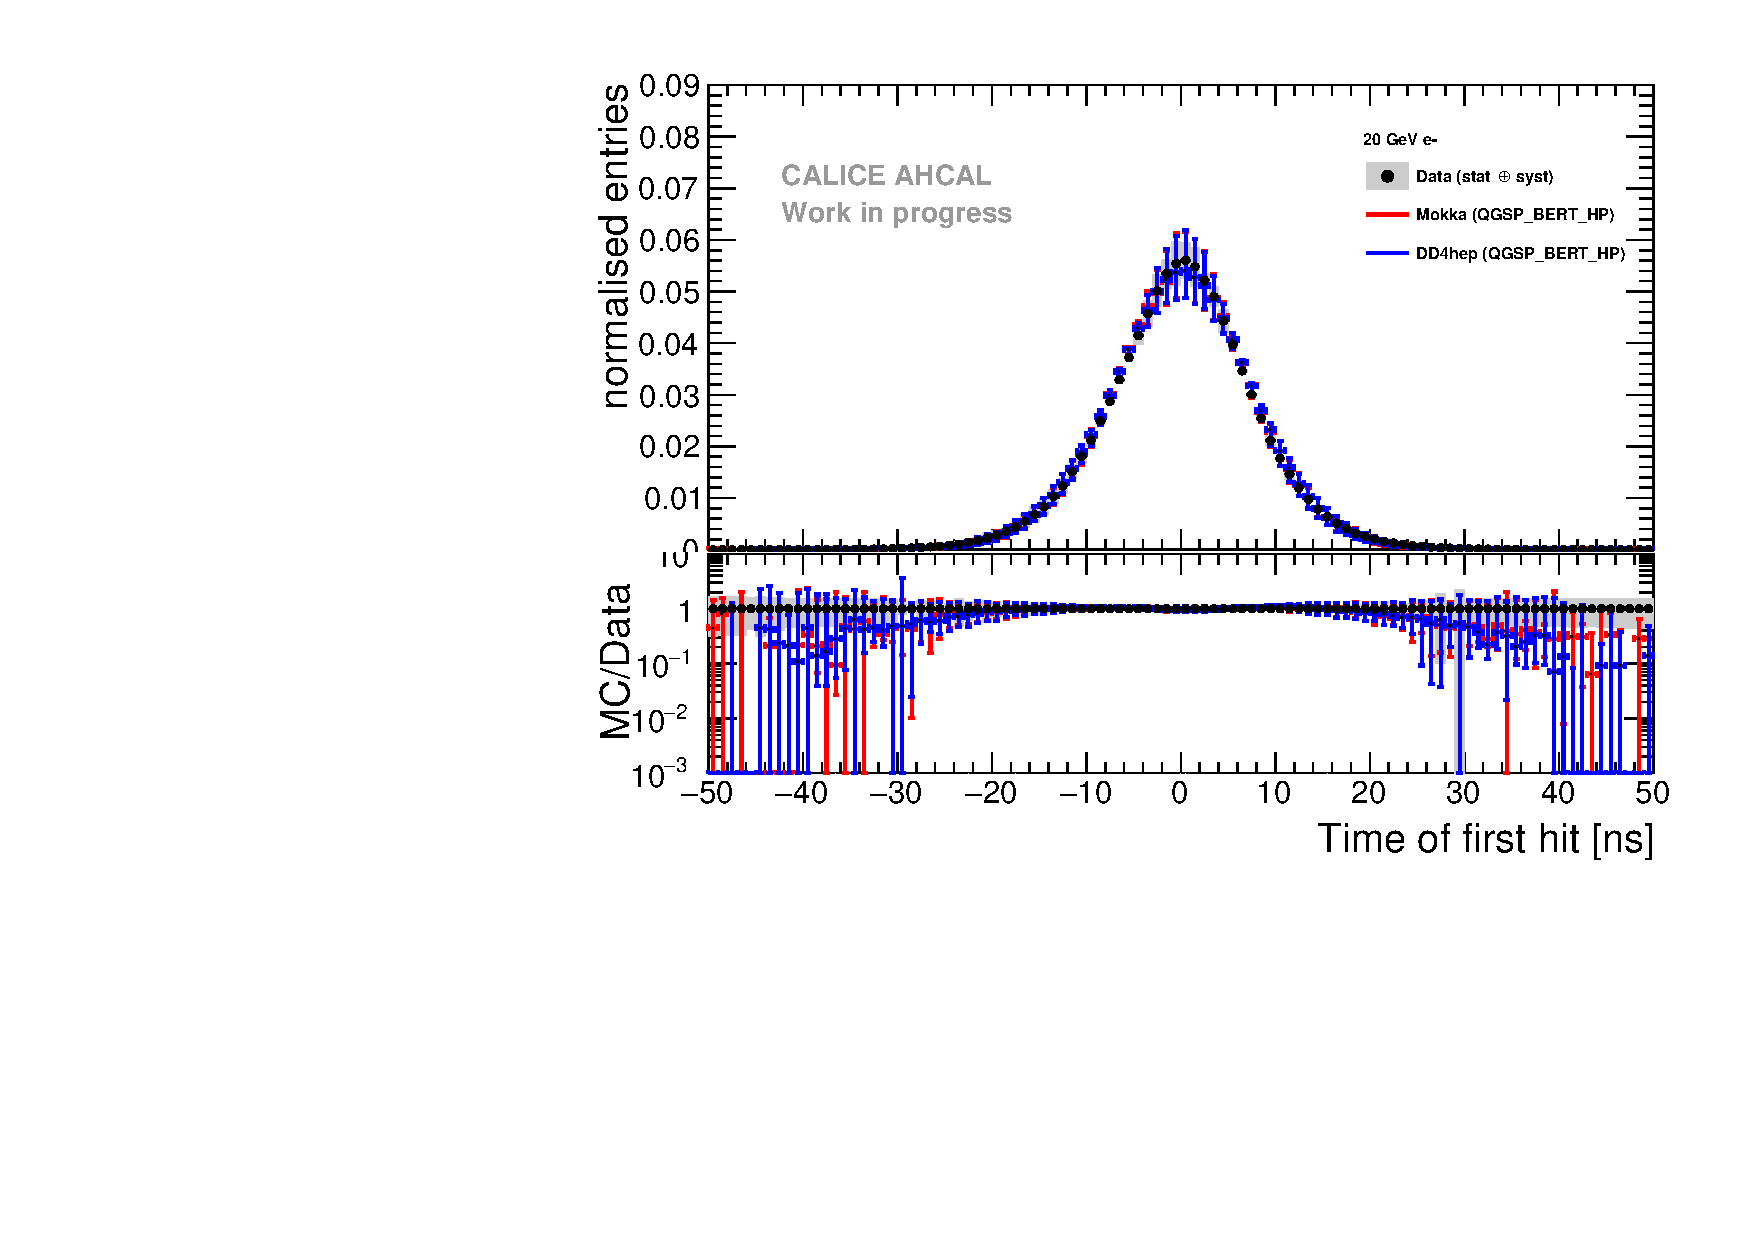
\includegraphics[width=1\textwidth]{../Thesis_Plots/Timing/Electrons/Plots/Comparison_SimData_Electrons20GeV.pdf}
		\caption{20 GeV.}\label{fig:elec_sim_data_20GeV}
	\end{subfigure}
	\hfill
	\begin{subfigure}[t]{0.5\textwidth}
		\centering
		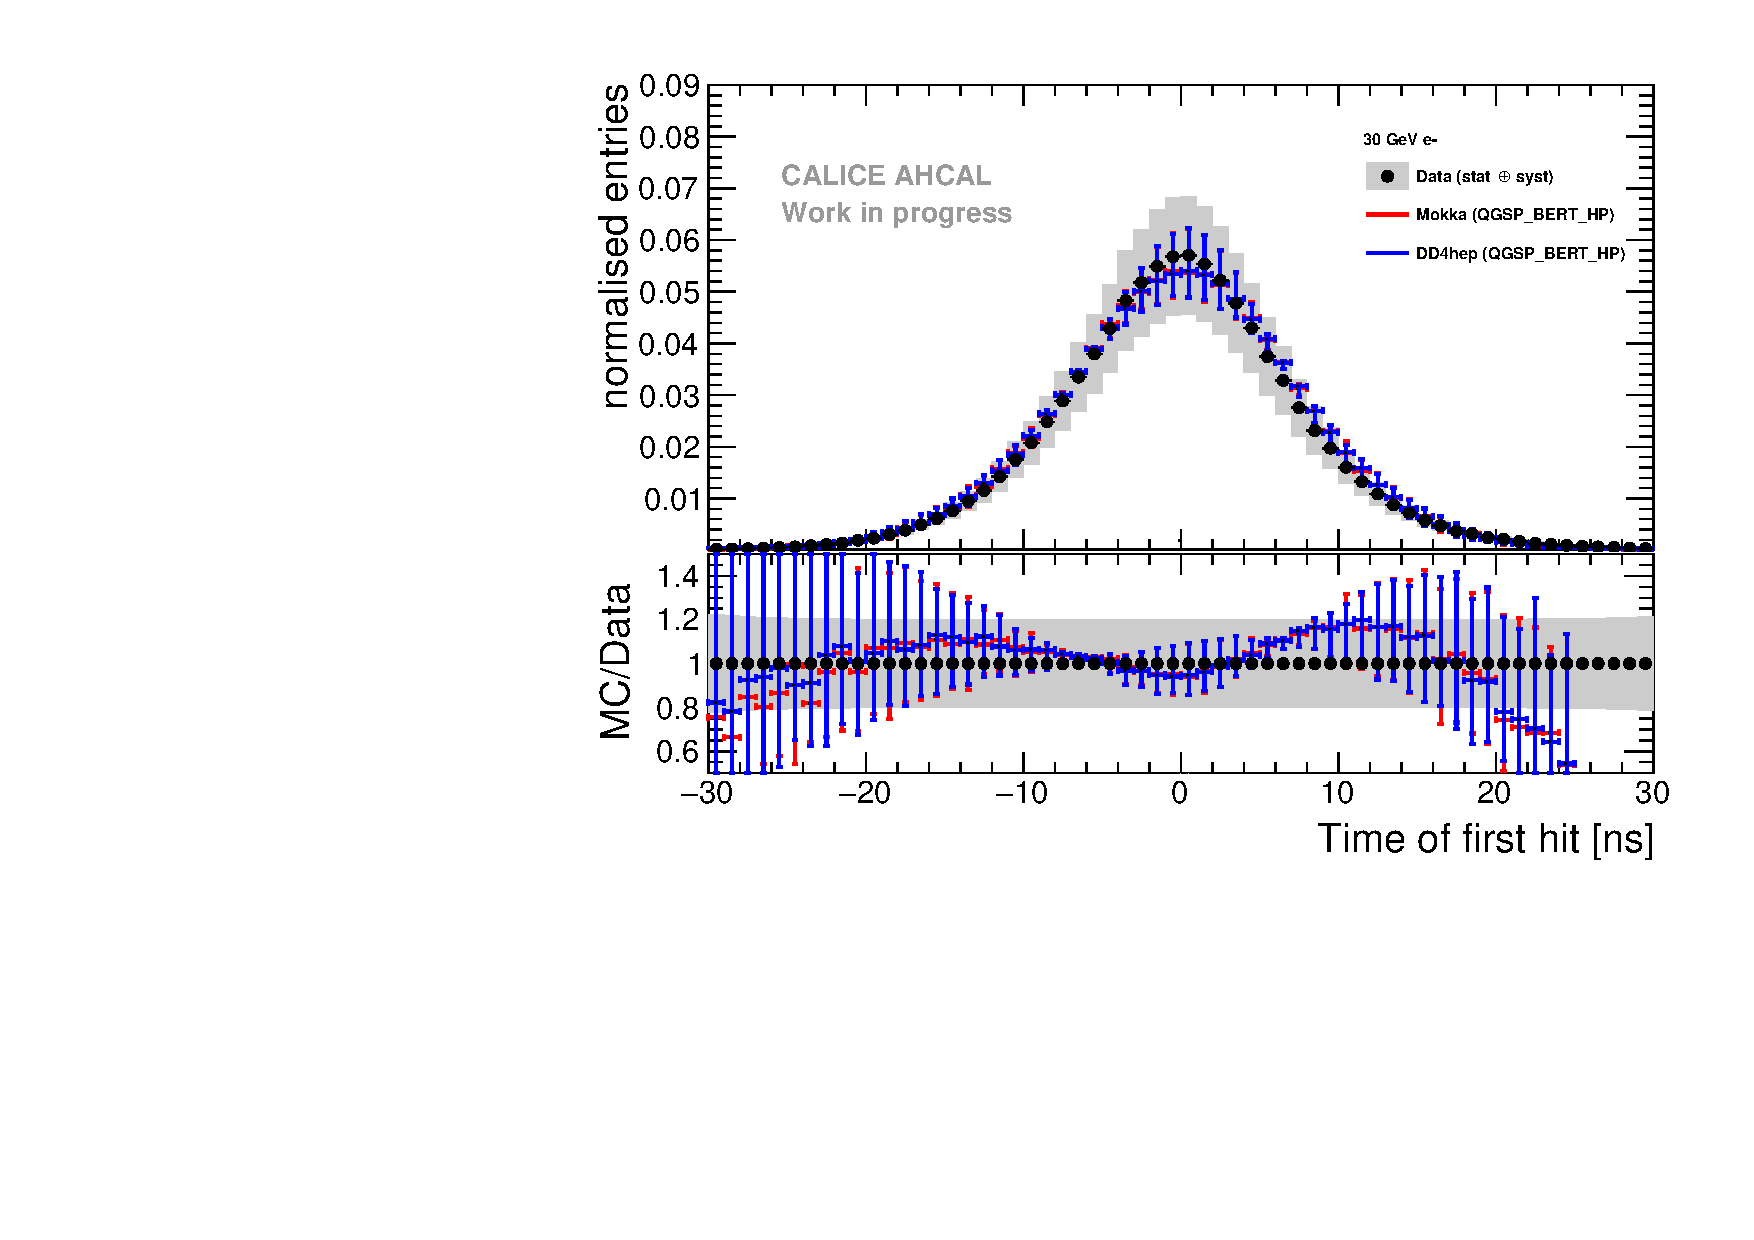
\includegraphics[width=1\textwidth]{../Thesis_Plots/Timing/Electrons/Plots/Comparison_SimData_Electrons30GeV.pdf}
		\caption{30 GeV.}\label{fig:elec_sim_data_30GeV}
	\end{subfigure}
	\hfill
	\begin{subfigure}[t]{0.5\textwidth}
		\centering
		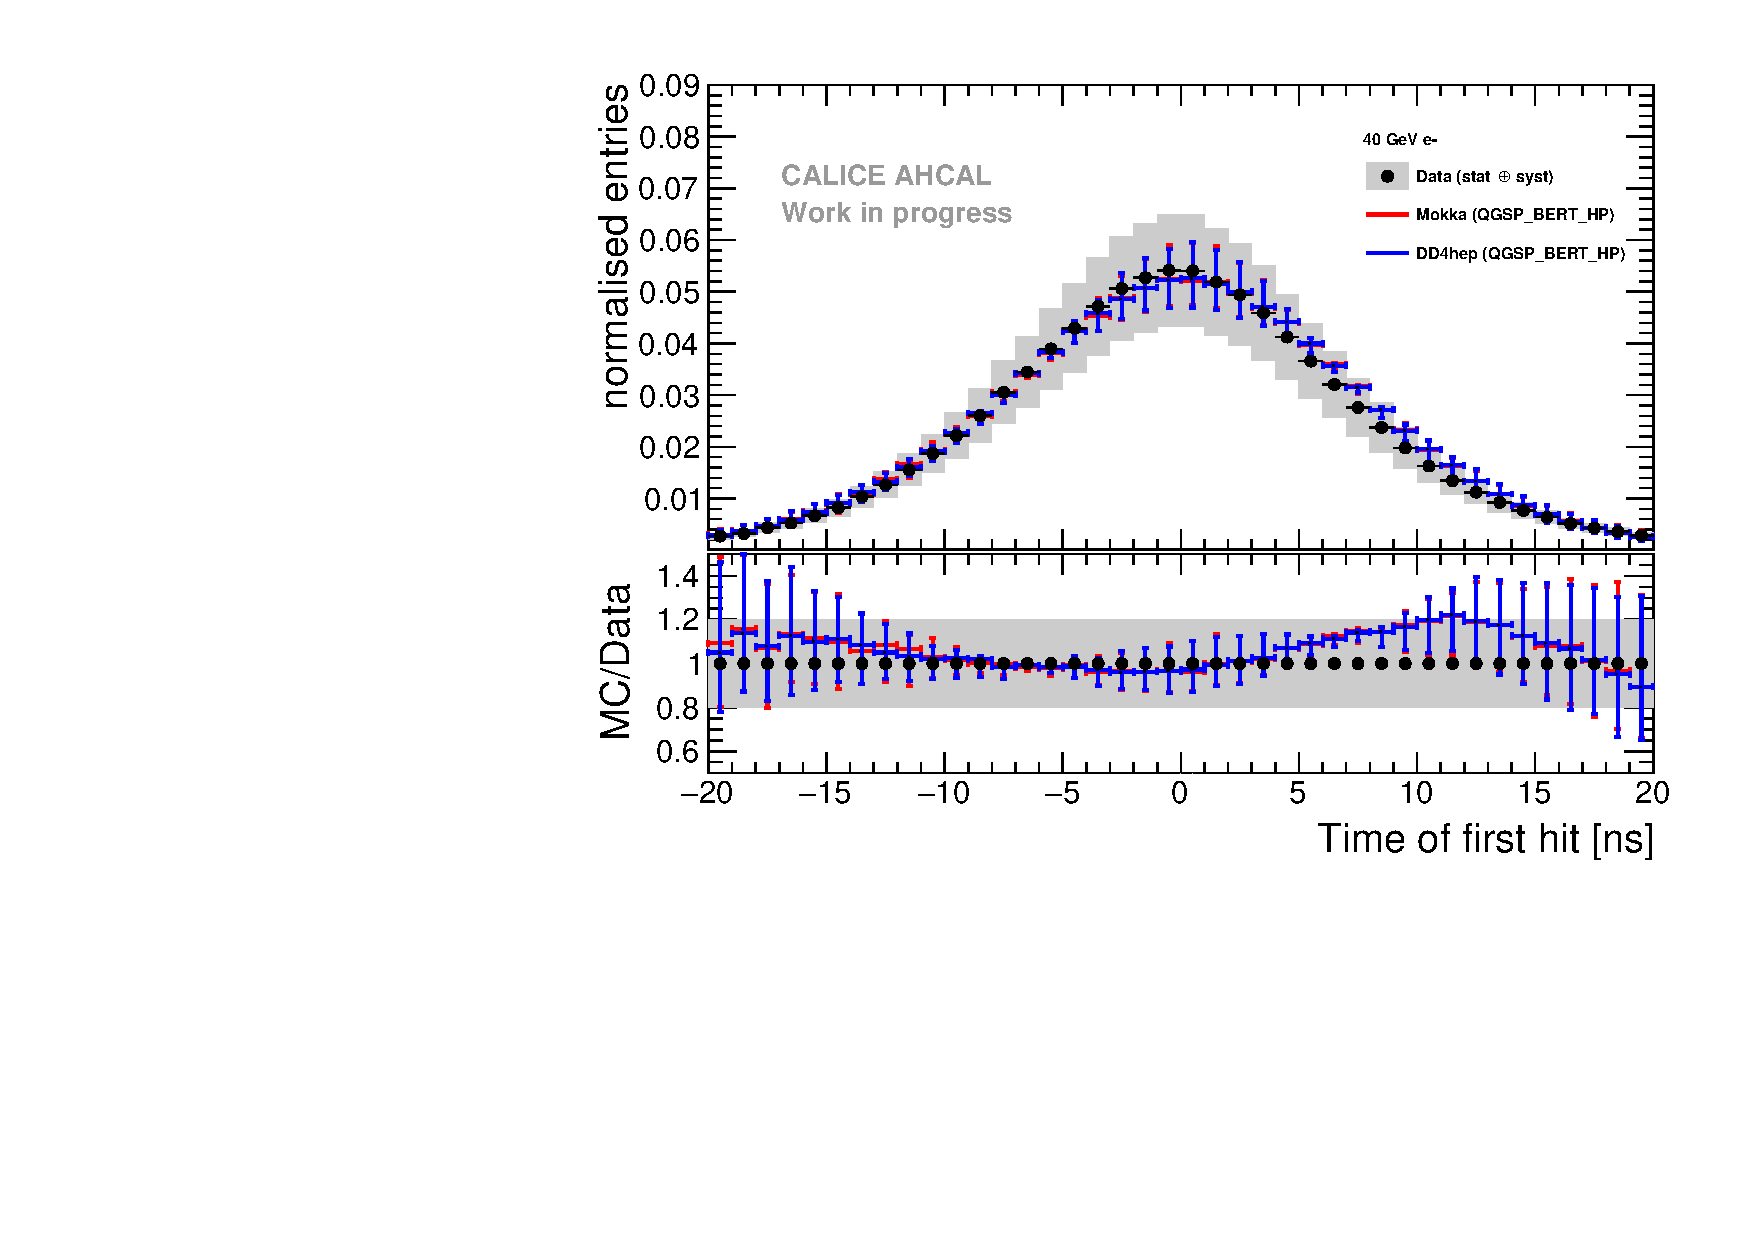
\includegraphics[width=1\textwidth]{../Thesis_Plots/Timing/Electrons/Plots/Comparison_SimData_Electrons40GeV.pdf}
		\caption{40 GeV.}\label{fig:elec_sim_data_40GeV}
	\end{subfigure}
	\hfill
	\begin{subfigure}[t]{0.5\textwidth}
		\centering
		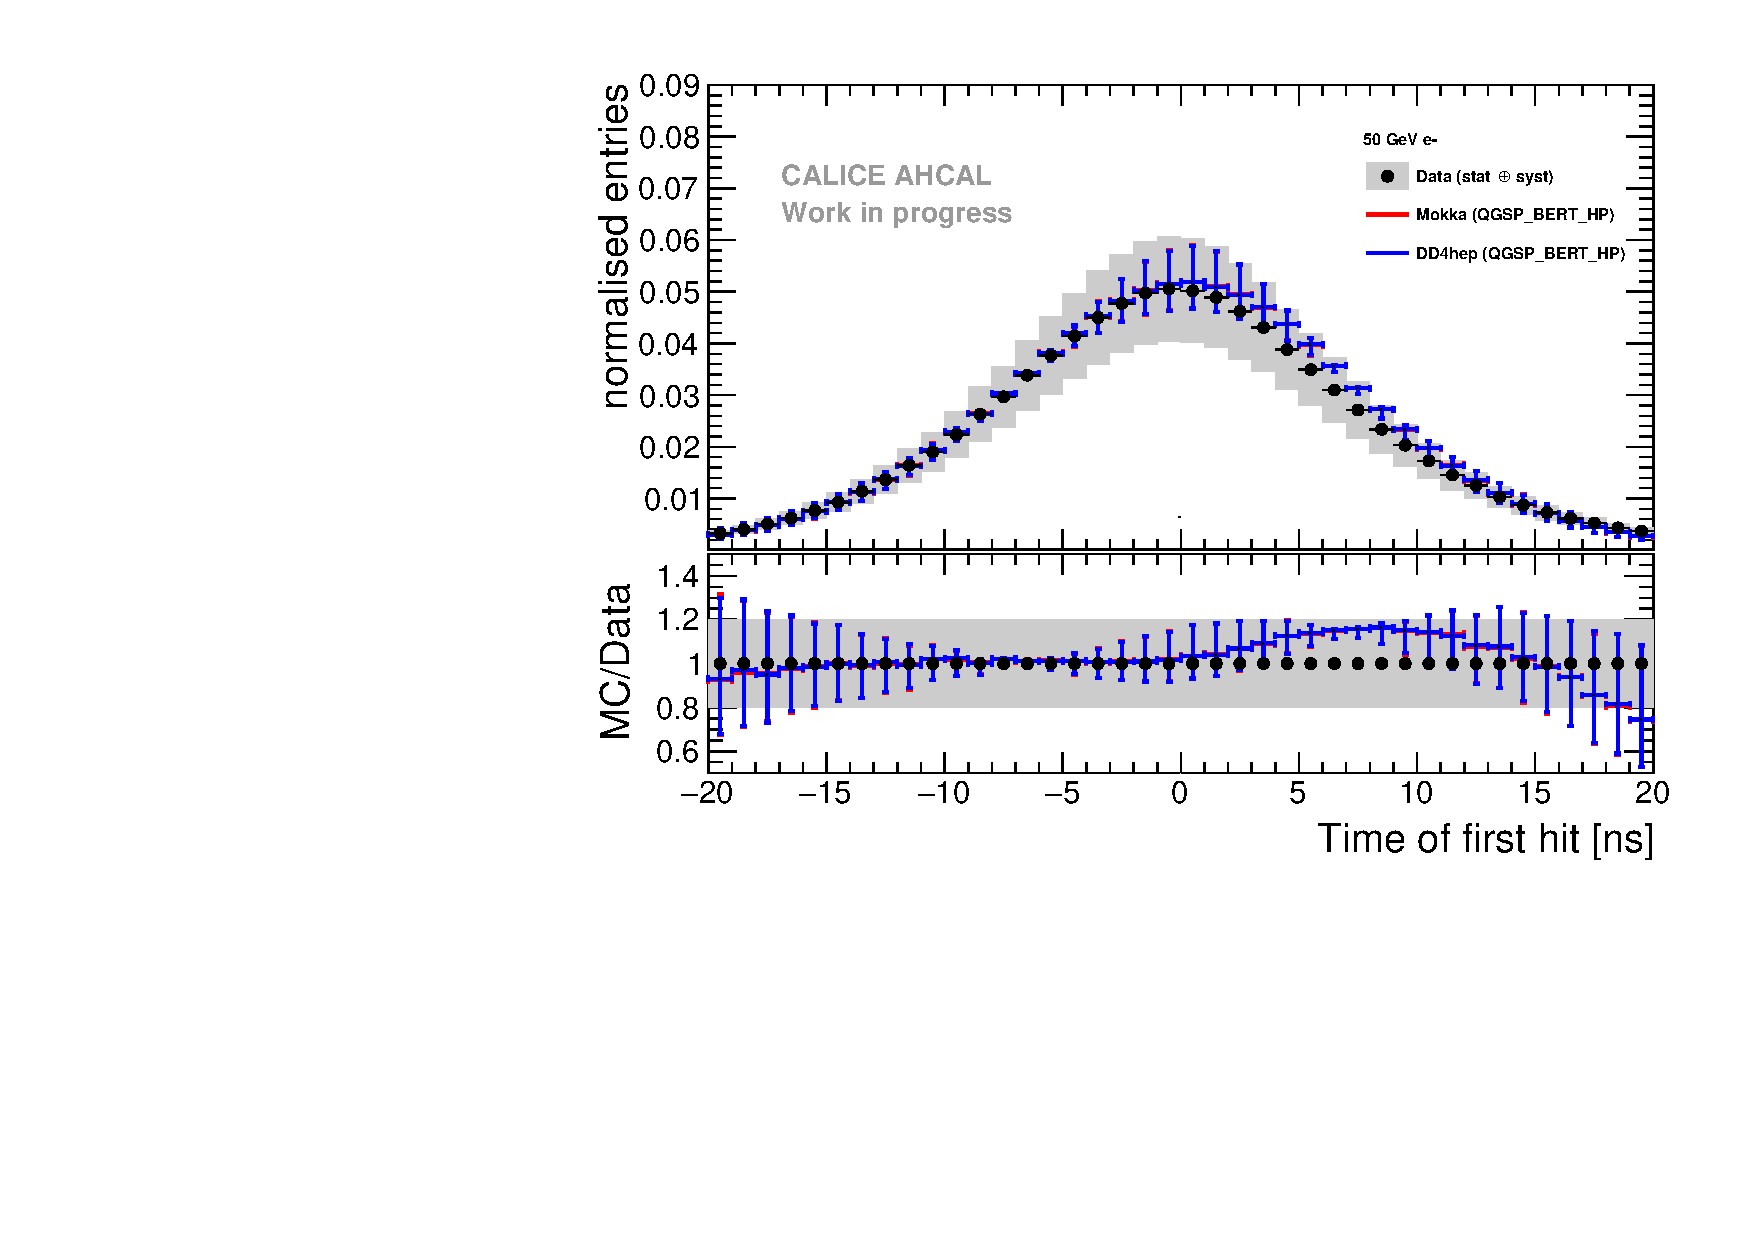
\includegraphics[width=1\textwidth]{../Thesis_Plots/Timing/Electrons/Plots/Comparison_SimData_Electrons50GeV.pdf}
		\caption{50 GeV.}\label{fig:elec_sim_data_50GeV}
	\end{subfigure}
	\caption{Comparison between electron data and MC for all energies of the time of first hit. The grey area represents the statistical and systematical error of the data. Error bars in simulation are obtained by varying the cross-talk parameter and with the error envelope from the number of hits parametrization.}
	\label{fig:sim_data_elec}
\end{figure}

The simulation is systematically narrower than data for all energies. This would suggest that simulation has less hits than data which is in agreement with figure \ref{fig:sim_data_elec_nHits}, where generally simulation is 10-20\% lower than data in the region of 6 to 10 hits per chip. For the time of first hit, The simulation is in better agreement for higher energies, at 40-50 GeV, than for lower energies at 10-15 GeV. This may come from imperfect beam profiles where a slight shift in simulation can influence highly the number of triggers in a chip. Also the number of triggered channels parametrization may be imperfect and may suggest that it could be chip-wise or layer-wise. But due to the limited amount of data, only a global parametrization could be applied. For 10 to 20 GeV comparisons, the description of the tails in simulation are quite underestimated. This may be due to the description of the noise in simulation that is not perfectly reproduced. Overall, the simulation and data are in agreement within statistical and systematic uncertainties.
% Change plots from -50 to 50 ns?%
\begin{figure}[htbp!]
	\begin{subfigure}[t]{0.5\textwidth}
		\centering
		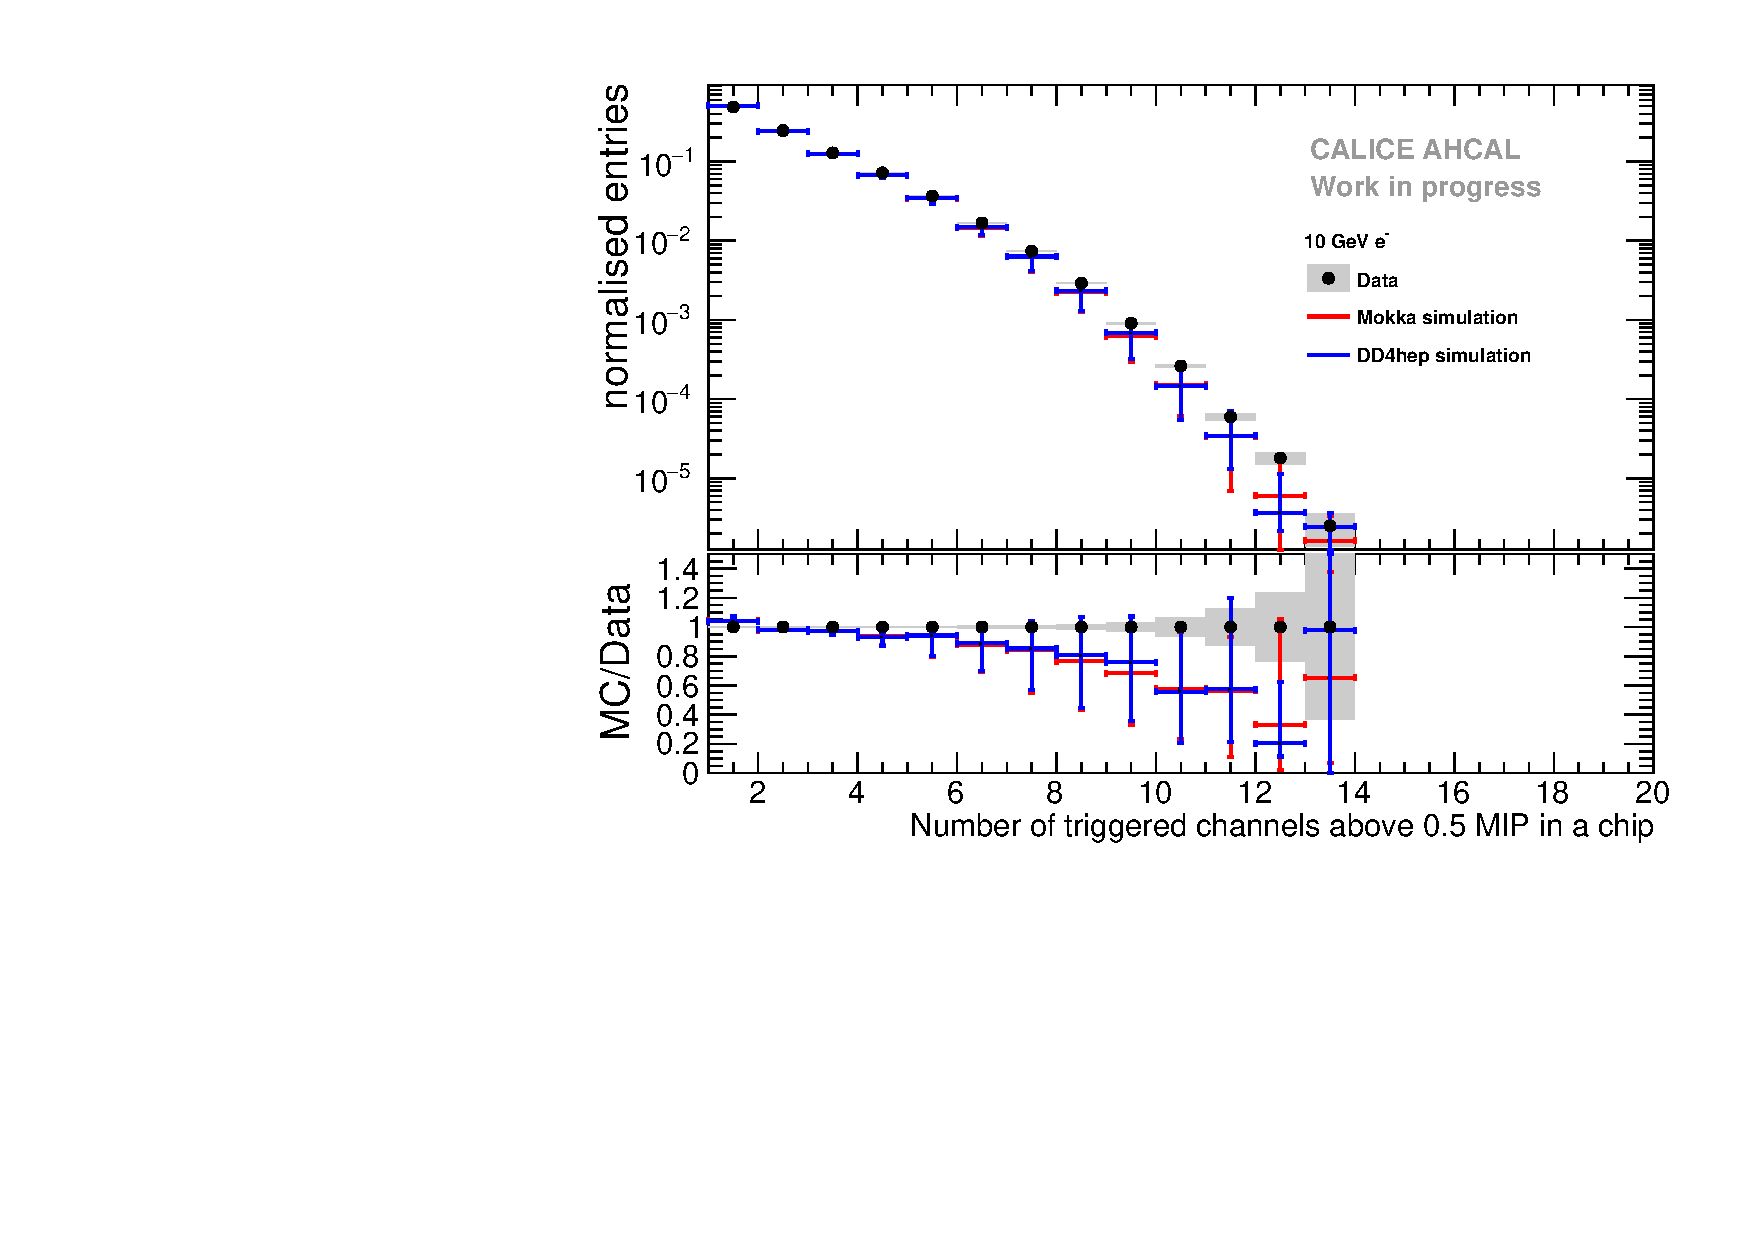
\includegraphics[width=1\textwidth]{../Thesis_Plots/Timing/Electrons/Plots/Comparison_SimData_Electrons_nHits_10GeV.pdf}
		\caption{10 GeV.}\label{fig:elec_sim_data_nHits_10GeV}
	\end{subfigure}
	\hfill
	\begin{subfigure}[t]{0.5\textwidth}
		\centering
		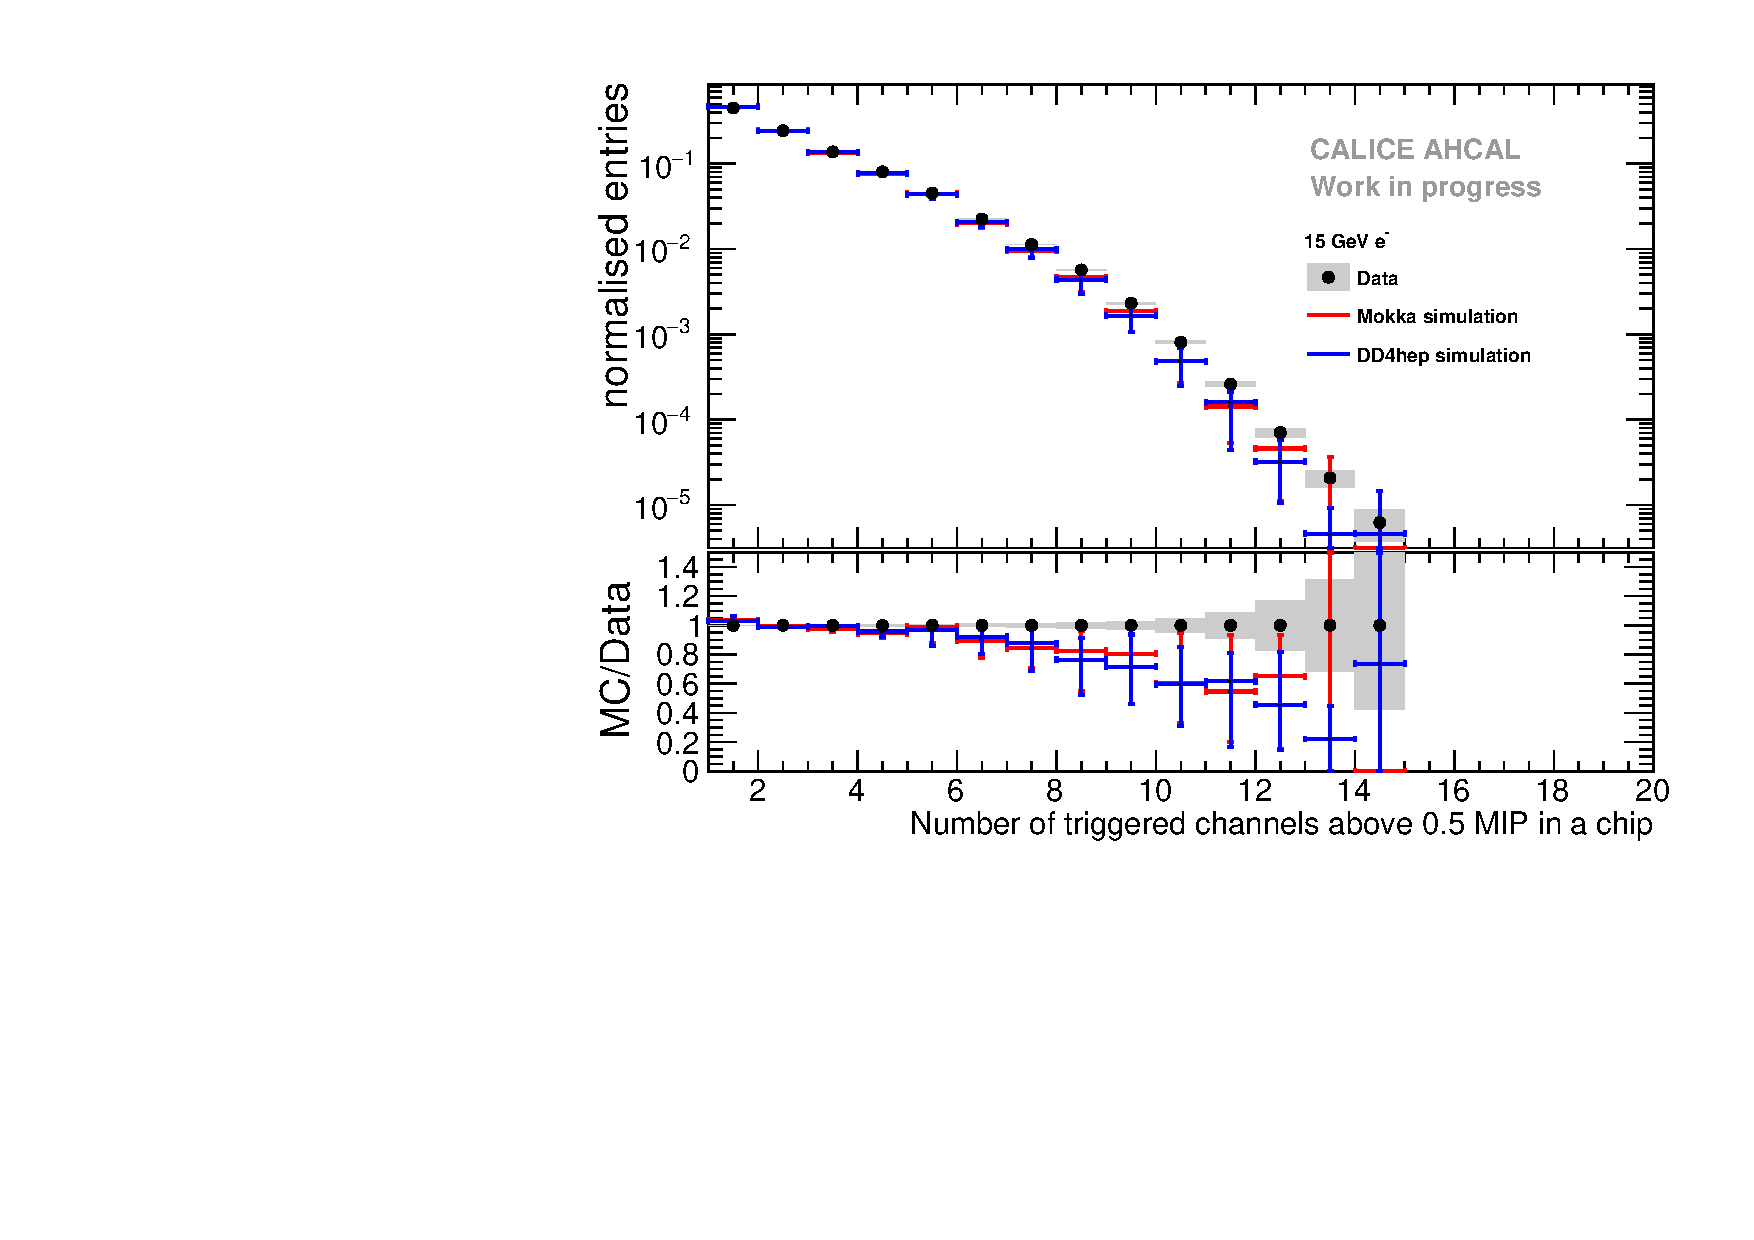
\includegraphics[width=1\textwidth]{../Thesis_Plots/Timing/Electrons/Plots/Comparison_SimData_Electrons_nHits_15GeV.pdf}
		\caption{15 GeV.}\label{fig:elec_sim_data_nHits_15GeV}
	\end{subfigure}
	\hfill
	\begin{subfigure}[t]{0.5\textwidth}
		\centering
		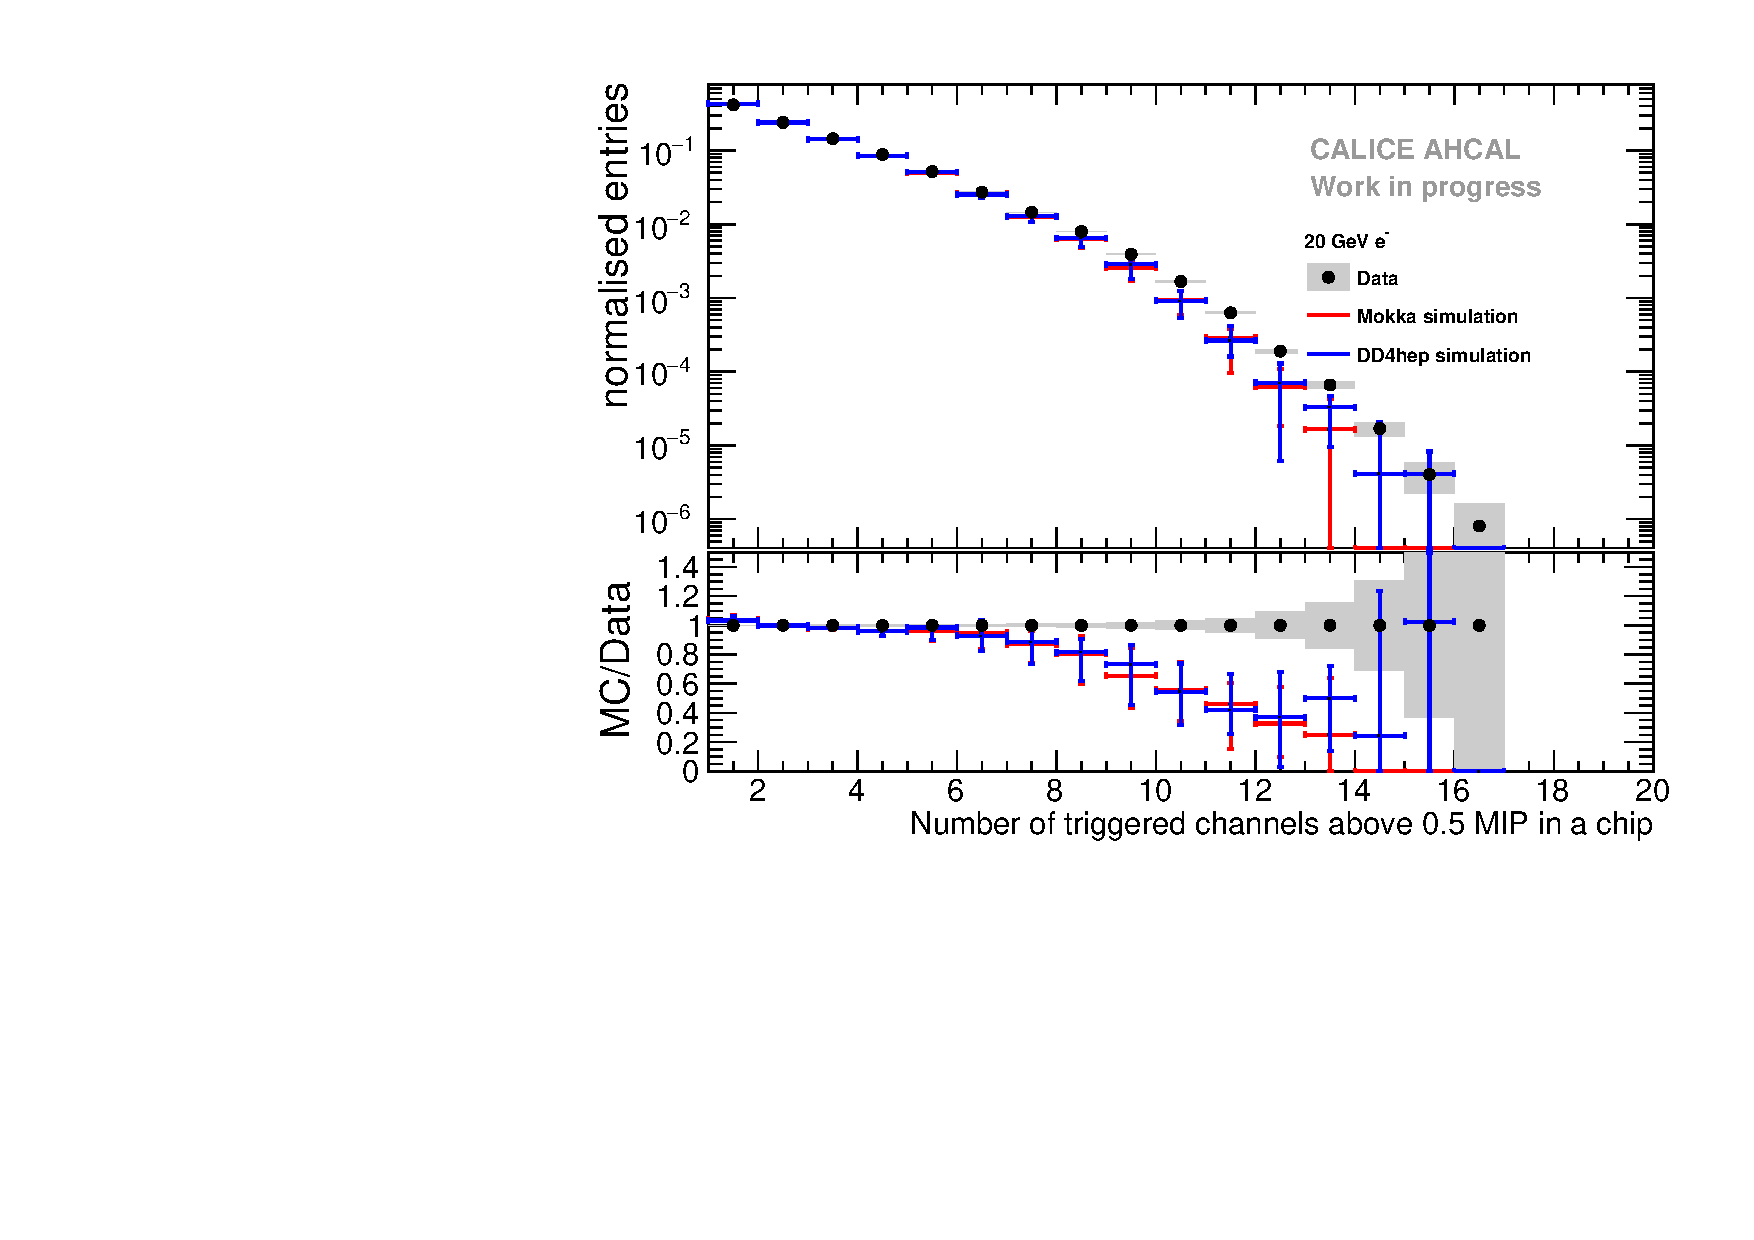
\includegraphics[width=1\textwidth]{../Thesis_Plots/Timing/Electrons/Plots/Comparison_SimData_Electrons_nHits_20GeV.pdf}
		\caption{20 GeV.}\label{fig:elec_sim_data_nHits_20GeV}
	\end{subfigure}
	\hfill
	\begin{subfigure}[t]{0.5\textwidth}
		\centering
		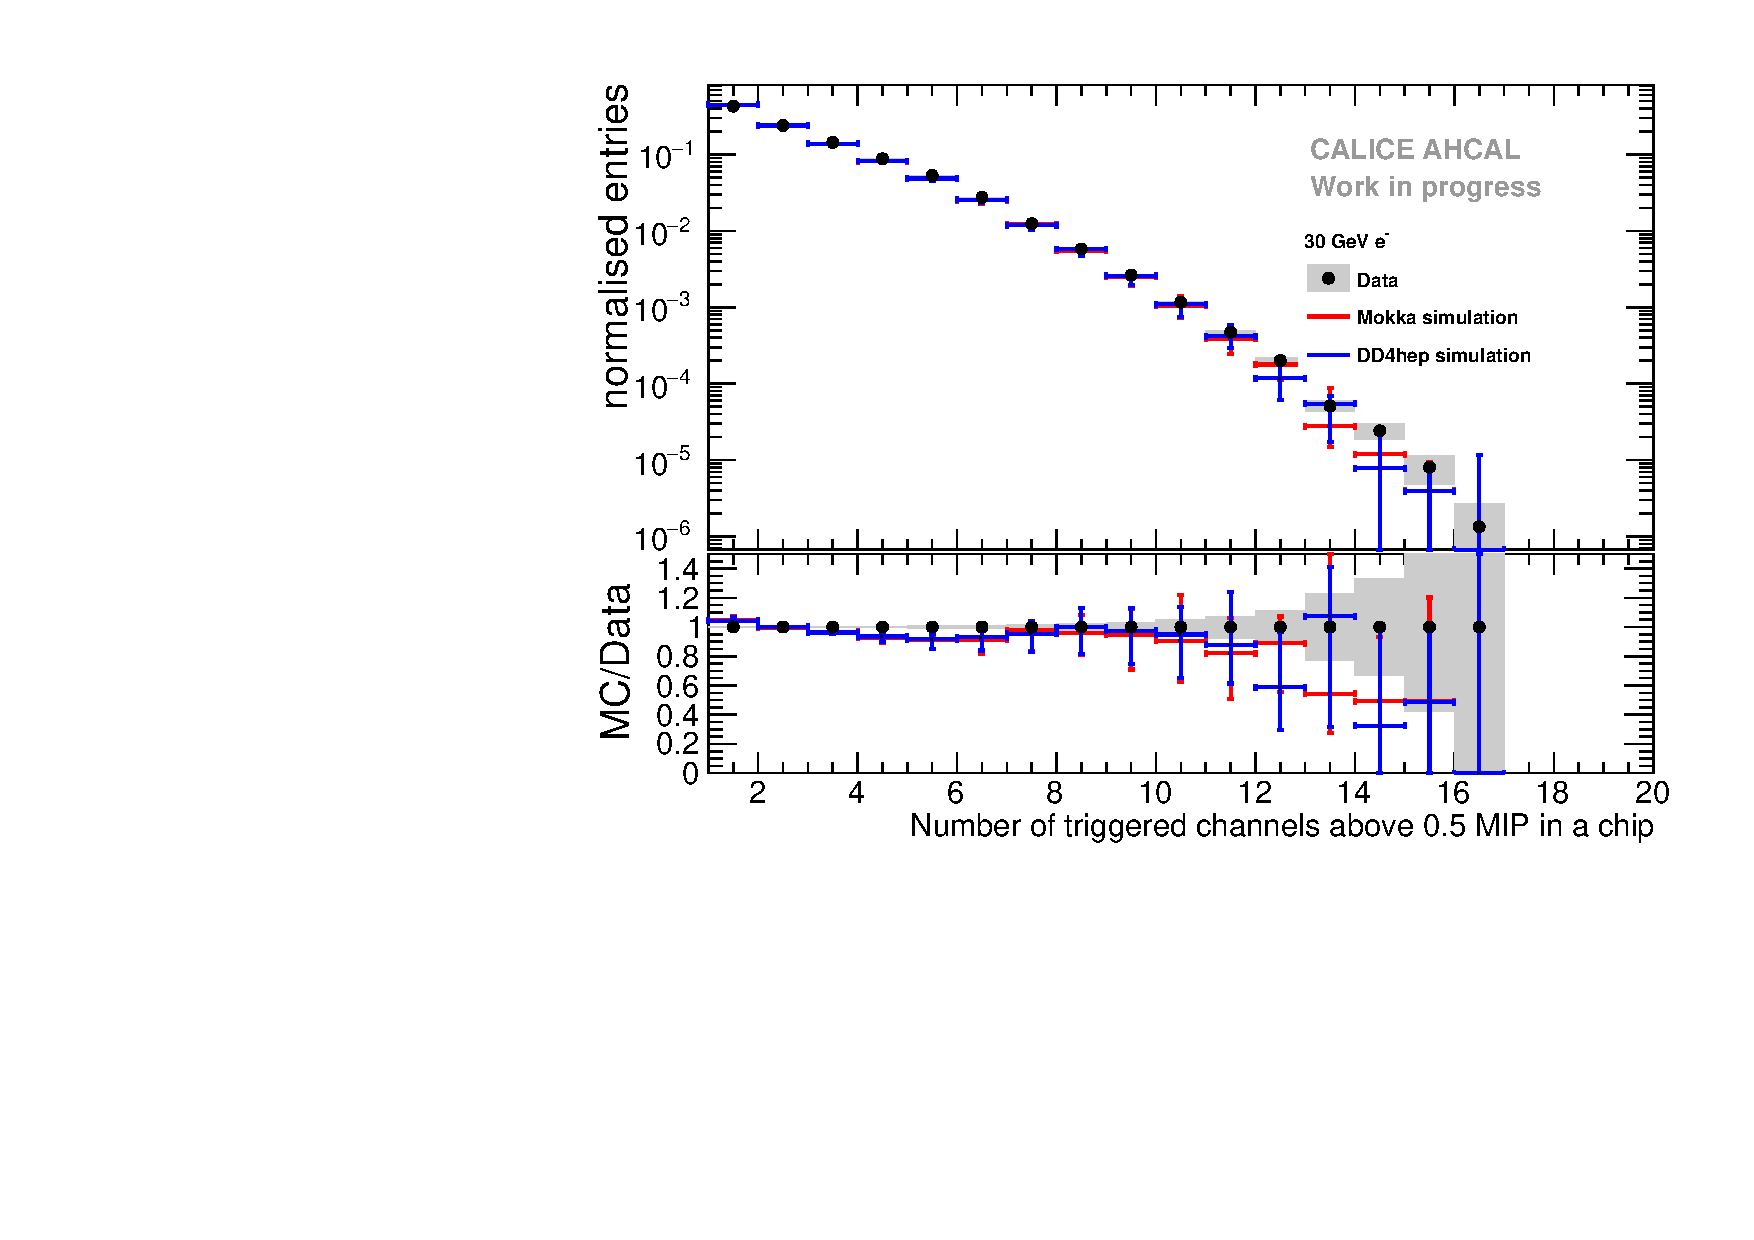
\includegraphics[width=1\textwidth]{../Thesis_Plots/Timing/Electrons/Plots/Comparison_SimData_Electrons_nHits_30GeV.pdf}
		\caption{30 GeV.}\label{fig:elec_sim_data_nHits_30GeV}
	\end{subfigure}
	\hfill
	\begin{subfigure}[t]{0.5\textwidth}
		\centering
		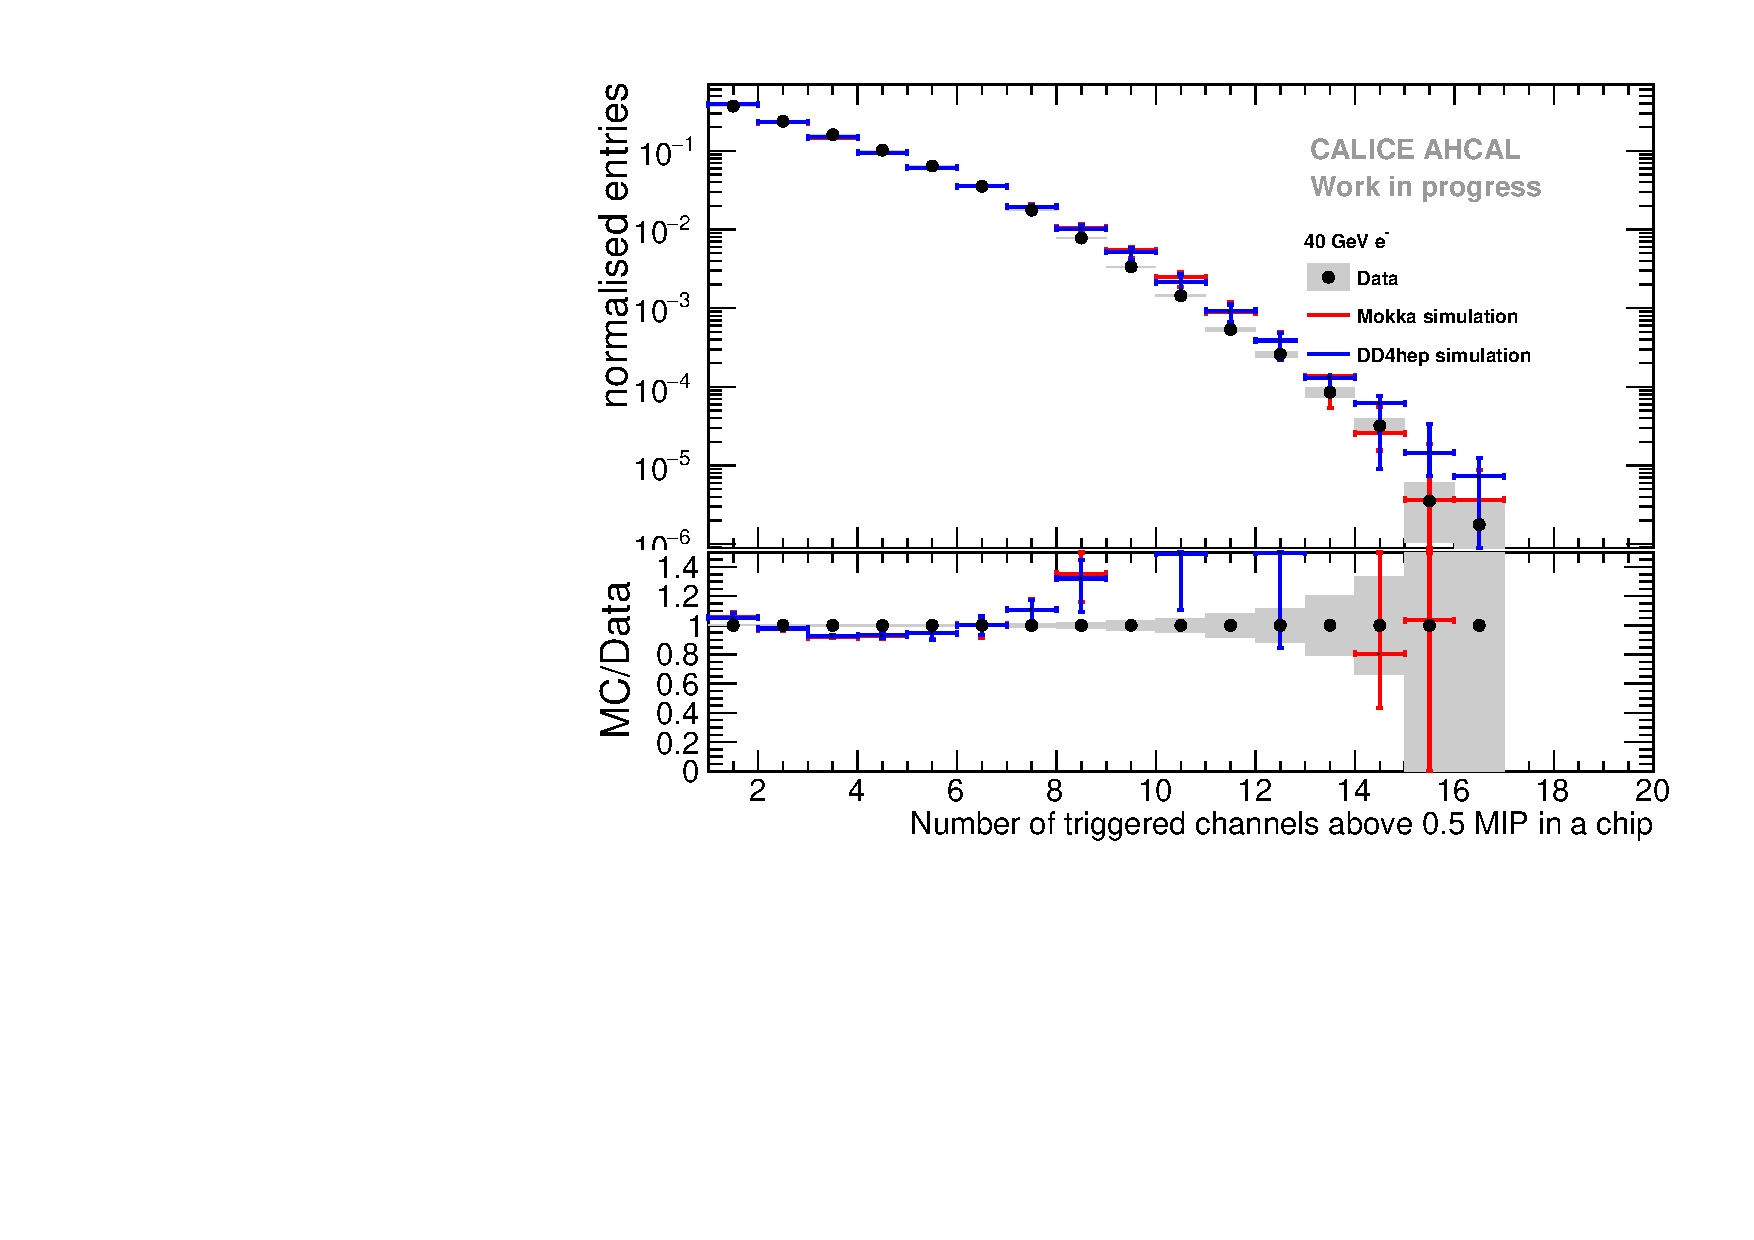
\includegraphics[width=1\textwidth]{../Thesis_Plots/Timing/Electrons/Plots/Comparison_SimData_Electrons_nHits_40GeV.pdf}
		\caption{40 GeV.}\label{fig:elec_sim_data_nHits_40GeV}
	\end{subfigure}
	\hfill
	\begin{subfigure}[t]{0.5\textwidth}
		\centering
		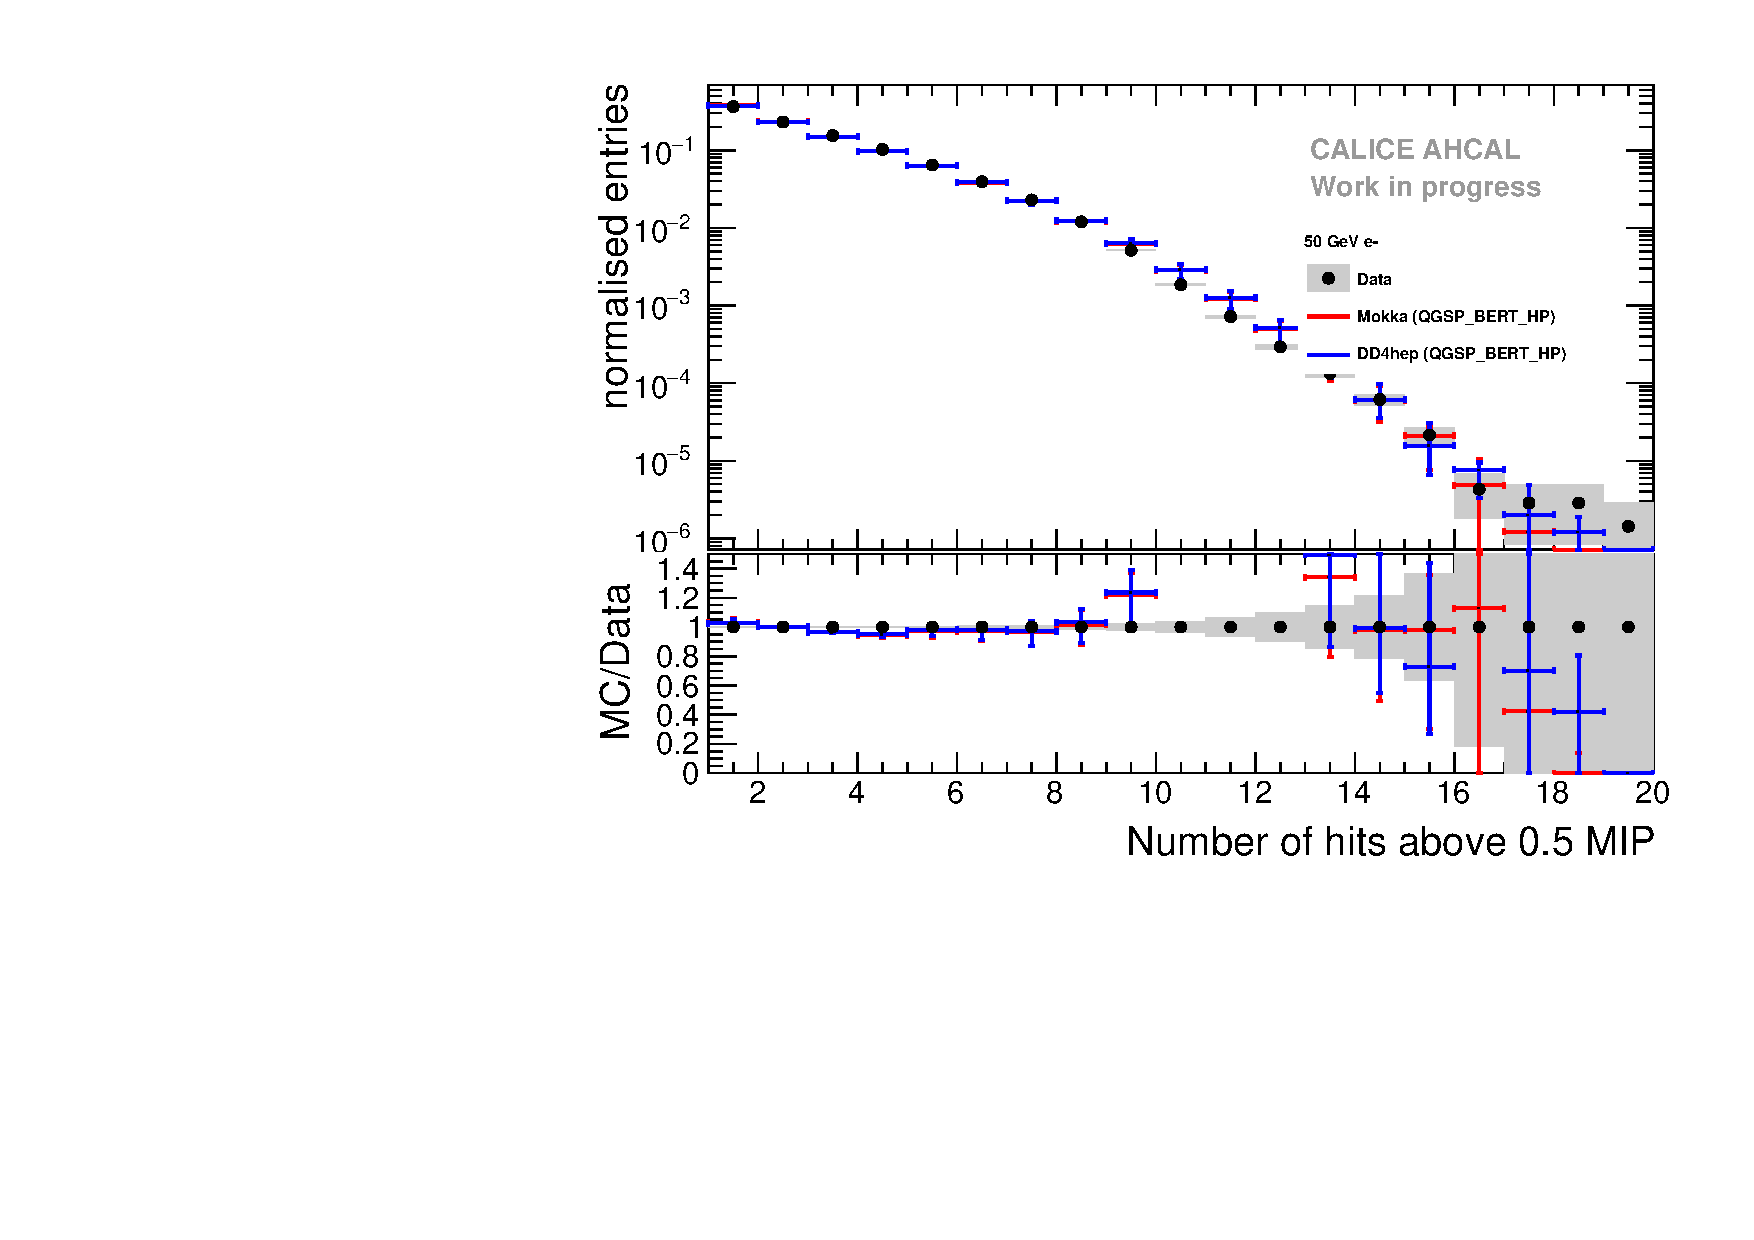
\includegraphics[width=1\textwidth]{../Thesis_Plots/Timing/Electrons/Plots/Comparison_SimData_Electrons_nHits_50GeV.pdf}
		\caption{50 GeV.}\label{fig:elec_sim_data_nHits_50GeV}
	\end{subfigure}
	\caption{Comparison between electron data and MC for all energies of the number of triggered channels per chip. The grey area represents the statistical error of the data. Error bars in simulation are obtained by varying the cross-talk parameter between 10\% and 18\%.}
	\label{fig:sim_data_elec_nHits}
\end{figure}
